
\newcommand{\mypapersize}{A4}
%% e.g., "A4", "letter", "legal", "executive", ...
%% The size of the paper of the resulting PDF file.

\newcommand{\mylaterality}{oneside}
%% "oneside" or "twoside"
%% Either you are creating a document which is printed on both, left pages
%% and right pages (twoside) or you create a document which is printed
%% on right pages only (oneside).

\newcommand{\mydraft}{false}
%% "true" or "false"
%% Use draft mode? If true, included graphics are replaced by empty
%% rectangles (of same size) and overfull boxes (in margin space) are
%% marked with black box (-> easy to spot!)

\newcommand{\myparskip}{half}
%% e.g., "no", "full", "half", ...
%% How to separate paragraphs: indention ("no") or spacing ("half",
%% "full", ...).

\newcommand{\myBCOR}{0mm}
%% Inner binding correction. This value depends on the method which is
%% being used to bind your printed result. Some techniques do not
%% require a binding correction at all ("0mm"), other require for
%% example "5mm". Refer to KOMA script documentation for a detailed
%% explanation what a binding correction is and how to measure it.

\newcommand{\myfontsize}{12pt}
%% e.g., 10pt, 11pt, 12pt
%% The font size of the main text in pt (points).

\newcommand{\mylinespread}{1.0}
%% e.g., 1.0, 1.5, 2.0
%% Line spacing in %/100. For example 1.5 means 150% of the usual line
%% spacing. Please use with caution: 100% ("1.0") is fine because the
%% font was designed for it.

\newcommand{\mylanguage}{english, ngerman}
%% "english,ngerman", "ngerman,english", ...
%% NOTE: The *last* language is the active one!
%% See babel documentation for further details.

%% BibLaTeX-settings: (see biblatex reference for further description)
\newcommand{\mybiblatexstyle}{authoryear}
%% e.g., "alphabetic", "authoryear", ...
%% The biblatex style which is being used for referencing. See
%% biblatex documentation for further details and more values.
%%\usepackage{mathtools}
%% CAUTION: if you change the style, please check for (in)compatible
%%          "biblatex" package options in the file
%%          "template/preamble.tex"! For example: "alphabetic" does
%%          not have an option "dashed=..." and causes an error if it
%%          does not get removed from the list of options.

\newcommand{\mybiblatexdashed}{false}  %% "true" or "false"
%% If true: replace recurring reference authors with a dash.

\newcommand{\mybiblatexbackref}{true}  %% "true" or "false"
%% If true: create backward links from reference to citations.

\newcommand{\mybiblatexfile}{references-biblatex.bib}
%% Name of the biblatex file that holds the references.

\newcommand{\mydispositioncolor}{30,103,182}
%% e.g., "30,103,182" (blue/turquois), "0,0,0" (black), ...
%% Color of the headings and so forth in RGB (red,green,blue) values.
%% NOTE: if you are using "0,0,0" for black, printers might still
%%       recognize pages as color pages. In case this is a problem
%%       (paying for color print-outs vs. paying for b/w-printouts)
%%       please edit file "template/preamble.tex" and change
%%       "\definecolor{DispositionColor}{RGB}{\mydispositioncolor}"
%%       to "\definecolor{DispositionColor}{gray}{0}" and thus
%%       overwriting the value of \mydispositioncolor above.

\newcommand{\mycolorlinks}{true}  %% "true" or "false"
%% Enables or disables colored links (hyperref package).

\newcommand{\mytitlepage}{template/title_Diplomarbeit_KF_Uni_Graz}
%% Your own or one of following pre-defined title pages:
%% "template/title_plain_maketitle": simple maketitle page
%% "template/title_Diplomarbeit_KF_Uni_Graz.tex": fancy (german) title page for KF Uni Graz
%% "template/title_Thesis_TU_Graz":
%%             titlepage for Graz University of Technology (correct
%%             (old?) Corporate Design) by Karl Voit (2012)
%% "template/title_Thesis_TU_Graz_-_kazemakase":
%%             titlepage for Graz University of Technology
%%             (correct new Corporate Design) by kazemakase (2013):
%%             see https://github.com/novoid/LaTeX-KOMA-template/issues/5
%% "template/title_VWA": titlepage for Vorwissenschaftliche Arbeit

\newcommand{\mytodonotesoptions}{}
%% e.g., "" (empty), "disable", ...
%% Options for the todonotes-package. If "disable", all todonotes will
%% be hidden (including listoftodos).

%% Load main settings for document preamble:
%% Time-stamp: <2018-03-11 14:25:47 vk>
%%%% === Disclaimer: =======================================================
%% created by
%%
%%      Karl Voit
%%
%% using GNU/Linux, GNU Emacs & LaTeX 2e
%%

%doc% %% overriding preamble/preamble.tex %%
%doc% \newcommand{\mylinespread}{1.0}  \newcommand{\mycolorlinks}{true}
%doc% \documentclass[12pt,paper=a4,parskip=half,DIV=calc,oneside,%%
%doc% headinclude,footinclude=false,open=right,bibliography=totoc]{scrartcl}
%doc% \usepackage[utf8]{inputenc}\usepackage[ngerman,american]{babel}\usepackage{scrpage2}
%doc% \usepackage{ifthen}\usepackage{eurosym}\usepackage{xspace}\usepackage[usenames,dvipsnames]{xcolor}
%doc% \usepackage[protrusion=true,factor=900]{microtype}
%doc% \usepackage{enumitem}
%doc% \usepackage[pdftex]{graphicx}
%doc% \usepackage{todonotes}
%doc% \usepackage{dingbat,bbding} %% special characters
%doc% \definecolor{DispositionColor}{RGB}{30,103,182}
%doc%
%doc% \usepackage[backend=biber,style=authoryear,dashed=false,natbib=true,hyperref=true%%
%doc% ]{biblatex}
%doc%
%doc% \addbibresource{references-biblatex.bib} %% remove, if using BibTeX instead of biblatex
%doc%
%doc% %% overriding userdata %%
%doc% \newcommand{\myauthor}{Karl Voit}\newcommand{\mytitle}{LaTeX Template Documentation}
%doc% \newcommand{\mysubject}{A Comprehensive Guide to Use the
%doc% Template from https://github.com/novoid/LaTeX-KOMA-template}
%doc% \newcommand{\mykeywords}{LaTeX, pdflatex, template, documentation, biber, biblatex}
%doc%
%doc% \newcommand{\myLaT}{\LaTeX{}@TUG\xspace}
%doc%
%doc% %% for future use?
%doc% % \usepackage{filecontents}
%doc% % \begin{filecontents}{filename.example}
%doc% %
%doc% % \end{filecontents}
%doc%
%doc%
%doc% %% using existing TeX files %%
%doc% %% Time-stamp: <2015-04-30 17:19:58 vk>
%%%% === Disclaimer: =======================================================
%% created by
%%
%%      Karl Voit
%%
%% using GNU/Linux, GNU Emacs & LaTeX 2e
%%

%doc%
%doc% \section{\texttt{mycommands.tex} --- various definitions}\myinteresting
%doc% \label{sec:mycommands}
%doc%
%doc% In file \verb#template/mycommands.tex# many useful commands are being
%doc% defined. 
%doc% 
%doc% \paragraph{What should I do with this file?} Please take a look at its 
%doc% content to get the most out of your document.
%doc% 

%doc% 
%doc% One of the best advantages of \LaTeX{} compared to \myacro{WYSIWYG} software products is
%doc% the possibility to define and use macros within text. This empowers the user to
%doc% a great extend.  Many things can be defined using \verb#\newcommand{}# and
%doc% automates repeating tasks. It is recommended to use macros not only for
%doc% repetitive tasks but also for separating form from content such as \myacro{CSS}
%doc% does for \myacro{XHTML}. Think of including graphics in your document: after
%doc% writing your book, you might want to change all captions to the upper side of
%doc% each figure. In this case you either have to modify all
%doc% \texttt{includegraphics} commands or you were clever enough to define something
%doc% like \verb#\myfig#\footnote{See below for a detailed description}. Using a
%doc% macro for including graphics enables you to modify the position caption on only
%doc% \emph{one} place: at the definition of the macro.
%doc% 
%doc% The following section describes some macros that came with this document template
%doc% from \myLaT and you are welcome to modify or extend them or to create
%doc% your own macros!
%doc% 

%doc% 
%doc% \subsection{\texttt{myfig} --- including graphics made easy}
%doc% 
%doc% The classic: you can easily add graphics to your document with \verb#\myfig#:
%doc% \begin{verbatim}
%doc%  \myfig{flower}%% filename w/o extension in the folder figures
%doc%        {width=0.7\textwidth}%% maximum width/height, aspect ratio will be kept
%doc%        {This flower was photographed at my home town in 2010}%% caption
%doc%        {Home town flower}%% optional (short) caption for list of figures
%doc%        {fig:flower}%% label
%doc% \end{verbatim}
%doc% 
%doc% There are many advantages of this command (compared to manual
%doc% \texttt{figure} environments and \texttt{includegraphics} commands:
%doc% \begin{itemize}
%doc% \item consistent style throughout the whole document
%doc% \item easy to change; for example move caption on top
%doc% \item much less characters to type (faster, error prone)
%doc% \item less visual clutter in the \TeX{}-files
%doc% \end{itemize}
%doc% 
%doc% 
\newcommand{\myfig}[5]{
%% example:
% \myfig{}%% filename in figures folder
%       {width=0.5\textwidth,height=0.5\textheight}%% maximum width/height, aspect ratio will be kept
%       {}%% caption
%       {}%% optional (short) caption for list of figures
%       {}%% label
\begin{figure}%[htp]
  \centering
  \includegraphics[keepaspectratio,#2]{figures/#1}
  \caption[#4]{#3}
  \label{#5} %% NOTE: always label *after* caption!
\end{figure}
}


%doc% 
%doc% \subsection{\texttt{myclone} --- repeat things!}
%doc% 
%doc% Using \verb#\myclone[42]{foobar}# results the text \enquote{foobar} printed 42 times.
%doc% But you can not only repeat text output with \texttt{myclone}. 
%doc%
%doc% Default argument
%doc% for the optional parameter \enquote{number of times} (like \enquote{42} in the example above) 
%doc% is set to two.
%doc% 
%% \myclone[x]{text}
\newcounter{myclonecnt}
\newcommand{\myclone}[2][2]{%
  \setcounter{myclonecnt}{#1}%
  \whiledo{\value{myclonecnt}>0}{#2\addtocounter{myclonecnt}{-1}}%
}

%old% %d oc% 
%old% %d oc% \subsection{\texttt{fixxme} --- sidemark something as unfinished}
%old% %d oc% 
%old% %d oc% You know it: something has to be fixed and you can not do it right
%old% %d oc% now. In order to \texttt{not} forget about it, you might want to add a
%old% %d oc% note like \verb+\fixxme{check again}+ which inserts a note on the page
%old% %d oc% margin such as this\fixxme{check again} example.
%old% %d oc%
%old% \newcommand{\fixxme}[1]{%%
%old% \textcolor{red}{FIXXME}\marginpar{\textcolor{red}{#1}}%%
%old% }


%%%% End 
%%% Local Variables:
%%% mode: latex
%%% mode: auto-fill
%%% mode: flyspell
%%% eval: (ispell-change-dictionary "en_US")
%%% TeX-master: "../main"
%%% End:
%% vim:foldmethod=expr
%% vim:fde=getline(v\:lnum)=~'^%%%%'?0\:getline(v\:lnum)=~'^%doc.*\ .\\%(sub\\)\\?section{.\\+'?'>1'\:'1':

%doc% %%%% Time-stamp: <2015-08-22 17:20:32 vk>
%%%% === Disclaimer: =======================================================
%% created by
%%
%%      Karl Voit
%%
%% using GNU/Linux, GNU Emacs & LaTeX 2e
%%
%doc%
%doc% \section{\texttt{typographic\_settings.tex} --- Typographic finetuning}
%doc%
%doc% The settings of file \verb#template/typographic_settings.tex# contain
%doc% typographic finetuning related to things mentioned in literature.  The
%doc% settings in this file relates to personal taste and most of all: 
%doc% \emph{typographic experience}. 
%doc% 
%doc% \paragraph{What should I do with this file?} You might as well skip the whole
%doc% file by excluding the \verb#%%%% Time-stamp: <2015-08-22 17:20:32 vk>
%%%% === Disclaimer: =======================================================
%% created by
%%
%%      Karl Voit
%%
%% using GNU/Linux, GNU Emacs & LaTeX 2e
%%
%doc%
%doc% \section{\texttt{typographic\_settings.tex} --- Typographic finetuning}
%doc%
%doc% The settings of file \verb#template/typographic_settings.tex# contain
%doc% typographic finetuning related to things mentioned in literature.  The
%doc% settings in this file relates to personal taste and most of all: 
%doc% \emph{typographic experience}. 
%doc% 
%doc% \paragraph{What should I do with this file?} You might as well skip the whole
%doc% file by excluding the \verb#\input{template/typographic_settings.tex}# command
%doc% in \texttt{main.tex}.  For standard usage it is recommended to stay with the
%doc% default settings.
%doc% 
%doc% 
%% ========================================================================

%doc%
%doc% Some basic microtypographic settings are provided by the
%doc% \texttt{microtype}
%doc% package\footnote{\url{http://ctan.org/pkg/microtype}}. This template
%doc% uses the rather conservative package parameters: \texttt{protrusion=true,factor=900}.
\usepackage[protrusion=true,factor=900]{microtype}

%doc%
%doc% \subsection{French spacing}
%doc%
%doc% \paragraph{Why?} see~\textcite[p.\,28, p.\,30]{Bringhurst1993}: `2.1.4 Use a single word space between sentences.'
%doc%
%doc% \paragraph{How?} see~\textcite[p.\,185]{Eijkhout2008}:\\
%doc% \verb#\frenchspacing  %% Macro to switch off extra space after punctuation.# \\
\frenchspacing  %% Macro to switch off extra space after punctuation.
%doc%
%doc% Note: This setting might be default for \myacro{KOMA} script.
%doc%


%doc%
%doc% \subsection{Font}
%doc% 
%doc% This template is using the Palatino font (package \texttt{mathpazo}) which results
%doc% in a legible document and matching mathematical fonts for printout.
%doc% 
%doc% It is highly recommended that you either stick to the Palatino font or use the
%doc% \LaTeX{} default fonts (by removing the package \texttt{mathpazo}).
%doc% 
%doc% Chosing different fonts is not
%doc% an easy task. Please leave this to people with good knowledge on this subject.
%doc% 
%doc% One valid reason to change the default fonts is when your document is mainly
%doc% read on a computer screen. In this case it is recommended to switch to a font
%doc% \textsf{which is sans-serif like this}. This template contains several alternative
%doc% font packages which can be activated in this file.
%doc% 

% for changing the default font, please go to the next subsection!

%doc%
%doc% \subsection{Text figures}
%doc% 
%doc% \ldots also called old style numbers such as 0123456789. 
%doc% (German: \enquote{Mediäval\-ziffern\footnote{\url{https://secure.wikimedia.org/wikibooks/de/wiki/LaTeX-W\%C3\%B6rterbuch:\_Medi\%C3\%A4valziffern}}})
%doc% \paragraph{Why?} see~\textcite[p.\,44f]{Bringhurst1993}: 
%doc% \begin{quote}
%doc% `3.2.1 If the font includes both text figures and titling figures, use
%doc%  titling figures only with full caps, and text figures in all other
%doc%  circumstances.'
%doc% \end{quote}
%doc% 
%doc% \paragraph{How?} 
%doc% Quoted from Wikibooks\footnote{\url{https://secure.wikimedia.org/wikibooks/en/wiki/LaTeX/Formatting\#Text\_figures\_.28.22old\_style.22\_numerals.29}}:
%doc% \begin{quote}
%doc% Some fonts do not have text figures built in; the textcomp package attempts to
%doc% remedy this by effectively generating text figures from the currently-selected
%doc% font. Put \verb#\usepackage{textcomp}# in your preamble. textcomp also allows you to
%doc% use decimal points, properly formatted dollar signs, etc. within
%doc% \verb#\oldstylenums{}#.
%doc% \end{quote}
%doc% \ldots but proposed \LaTeX{} method does not work out well. Instead use:\\
%doc% \verb#\usepackage{hfoldsty}#  (enables text figures using additional font) or \\
%doc% \verb#\usepackage[sc,osf]{mathpazo}# (switches to Palatino font with small caps and old style figures enabled).
%doc%
%\usepackage{hfoldsty}  %% enables text figures using additional font
%% ... OR use ...
\usepackage[sc,osf]{mathpazo} %% switches to Palatino with small caps and old style figures

%% Font selection from:
%%     http://www.matthiaspospiech.de/latex/vorlagen/allgemein/preambel/fonts/
%% use following lines *instead* of the mathpazo package above:
%% ===== Serif =========================================================
%% for Computer Modern (LaTeX default font), simply remove the mathpazo above
%\usepackage{charter}\linespread{1.05} %% Charter
%\usepackage{bookman}                  %% Bookman (laedt Avant Garde !!)
%\usepackage{newcent}                  %% New Century Schoolbook (laedt Avant Garde !!)
%% ===== Sans Serif ====================================================
%\renewcommand{\familydefault}{\sfdefault}  %% this one in *combination* with the default mathpazo package
%\usepackage{cmbright}                  %% CM-Bright (eigntlich eine Familie)
%\usepackage{tpslifonts}                %% tpslifonts % Font for Slides


%doc% 
%doc% \subsection{\texttt{myacro} --- Abbrevations using \textsc{small caps}}\myinteresting
%doc% \label{sec:myacro}
%doc% 
%doc% \paragraph{Why?} see~\textcite[p.\,45f]{Bringhurst1993}: `3.2.2 For abbrevations and
%doc% acronyms in the midst of normal text, use spaced small caps.'
%doc% 
%doc% \paragraph{How?} Using the predefined macro \verb#\myacro{}# for things like
%doc% \myacro{UNO} or \myacro{UNESCO} using \verb#\myacro{UNO}# or \verb#\myacro{UNESCO}#.
%doc% 
\DeclareRobustCommand{\myacro}[1]{\textsc{\lowercase{#1}}} %%  abbrevations using small caps


%doc% 
%doc% \subsection{Colorized headings and links}
%doc% 
%doc% This document template is able to generate an output that uses colorized
%doc% headings, captions, page numbers, and links. The color named `DispositionColor'
%doc% used in this document is defined near the definition of package \texttt{color}
%doc% in the preamble (see section~\ref{subsec:miscpackages}). The changes required
%doc% for headings, page numbers, and captions are defined here.
%doc% 
%doc% Settings for colored links are handled by the definitions of the
%doc% \texttt{hyperref} package (see section~\ref{sec:pdf}).
%doc% 
\setheadsepline{.4pt}[\color{DispositionColor}]
\renewcommand{\headfont}{\normalfont\sffamily\color{DispositionColor}}
\renewcommand{\pnumfont}{\normalfont\sffamily\color{DispositionColor}}
\addtokomafont{disposition}{\color{DispositionColor}}
\addtokomafont{caption}{\color{DispositionColor}\footnotesize}
\addtokomafont{captionlabel}{\color{DispositionColor}}

%doc% 
%doc% \subsection{No figures or tables below footnotes}
%doc% 
%doc% \LaTeX{} places floating environments below footnotes if \texttt{b}
%doc% (bottom) is used as (default) placement algorithm. This is certainly
%doc% not appealing for most people and is deactivated in this template by
%doc% using the package \texttt{footmisc} with its option \texttt{bottom}.
%doc% 
%% see also: http://www.komascript.de/node/858 (German description)
\usepackage[bottom]{footmisc}

%doc% 
%doc% \subsection{Spacings of list environments}
%doc% 
%doc% By default, \LaTeX{} is using vertical spaces between items of enumerate, 
%doc% itemize and description environments. This is fine for multi-line items.
%doc% Many times, the user does just write single-line items where the larger
%doc% vertical space is inappropriate. The \href{http://ctan.org/pkg/enumitem}{enumitem}
%doc% package provides replacements for the pre-defined list environments and
%doc% offers many options to modify their appearances.
%doc% This template is using the package option for \texttt{noitemsep} which
%doc% mimimizes the vertical space between list items.
%doc% 
\usepackage{enumitem}
\setlist{noitemsep}   %% kills the space between items

%doc% 
%doc% \subsection{\texttt{csquotes} --- Correct quotation marks}\myinteresting
%doc% \label{sub:csquotes}
%doc% 
%doc% \emph{Never} use quotation marks found on your keyboard.
%doc% They end up in strange characters or false looking quotation marks.
%doc% 
%doc% In \LaTeX{} you are able to use typographically correct quotation marks. The package 
%doc% \href{http://www.ctan.org/pkg/csquotes}{\texttt{csquotes}} offers you with 
%doc% \verb#\enquote{foobar}# a command to get correct quotation marks around \enquote{foobar}.
%doc% Please do check the package options in order to modify
%doc% its settings according to the language used\footnote{most of the time in 
%doc% combination with the language set in the options of the \texttt{babel} package}.
%doc% 
%doc% \href{http://www.ctan.org/pkg/csquotes}{\texttt{csquotes}} is also recommended 
%doc% by \texttt{biblatex} (see Section~\ref{sec:references}). 
\usepackage[babel=true,strict=true,english=american,german=guillemets]{csquotes}

%doc% 
%doc% \subsection{Line spread}
%doc% 
%doc% If you have to enlarge the distance between two lines of text, you can
%doc% increase it using the \texttt{\mylinespread} command in \texttt{main.tex}. By default, it is
%doc% deactivated (set to 100~percent). Modify only with caution since it influences the
%doc% page layout and could lead to ugly looking documents.
\linespread{\mylinespread}

%doc% 
%doc% \subsection{Optional: Lines above and below the chapter head}
%doc% 
%doc% This is not quite something typographic but rather a matter of taste.
%doc% \myacro{KOMA} Script offers \href{http://www.komascript.de/node/24}{a method to
%doc% add lines above and below chapter head} which is disabled by
%doc% default. If you want to enable this feature, remove corresponding
%doc% comment characters from the settings.
%doc% 
%% Source: http://www.komascript.de/node/24
%disabled% %% 1st get a new command
%disabled% \newcommand*{\ORIGchapterheadstartvskip}{}%
%disabled% %% 2nd save the original definition to the new command
%disabled% \let\ORIGchapterheadstartvskip=\chapterheadstartvskip
%disabled% %% 3rd redefine the command using the saved original command
%disabled% \renewcommand*{\chapterheadstartvskip}{%
%disabled%   \ORIGchapterheadstartvskip
%disabled%   {%
%disabled%     \setlength{\parskip}{0pt}%
%disabled%     \noindent\color{DispositionColor}\rule[.3\baselineskip]{\linewidth}{1pt}\par
%disabled%   }%
%disabled% }
%disabled% %% see above
%disabled% \newcommand*{\ORIGchapterheadendvskip}{}%
%disabled% \let\ORIGchapterheadendvskip=\chapterheadendvskip
%disabled% \renewcommand*{\chapterheadendvskip}{%
%disabled%   {%
%disabled%     \setlength{\parskip}{0pt}%
%disabled%     \noindent\color{DispositionColor}\rule[.3\baselineskip]{\linewidth}{1pt}\par
%disabled%   }%
%disabled%   \ORIGchapterheadendvskip
%disabled% }

%doc% 
%doc% \subsection{Optional: Chapter thumbs}
%doc% 
%doc% This is not quite something typographic but rather a matter of taste.
%doc% \myacro{KOMA} Script offers \href{http://www.komascript.de/chapterthumbs-example}{a method to
%doc% add chapter thumbs} (in combination with the package \texttt{scrpage2}) which is disabled by
%doc% default. If you want to enable this feature, remove corresponding
%doc% comment characters from the settings.
%doc% 
%disabled% \makeatletter
%disabled% % Safty first
%disabled% \@ifundefined{chapter}{\let\chapter\undefined
%disabled%   \chapter must be defined to use chapter thumbs!}{%
%disabled%  
%disabled% % Two new commands for the width and height of the boxes with the
%disabled% % chapter number at the thumbs (use of commands instead of lengths
%disabled% % for sparing registers)
%disabled% \newcommand*{\chapterthumbwidth}{2em}
%disabled% \newcommand*{\chapterthumbheight}{1em}
%disabled%  
%disabled% % Two new commands for the colors of the box background and the
%disabled% % chapter numbers of the thumbs
%disabled% \newcommand*{\chapterthumbboxcolor}{black}
%disabled% \newcommand*{\chapterthumbtextcolor}{white}
%disabled%  
%disabled% % New command to set a chapter thumb. I'm using a group at this
%disabled% % command, because I'm changing the temporary dimension \@tempdima
%disabled% \newcommand*{\putchapterthumb}{%
%disabled%   \begingroup
%disabled%     \Large
%disabled%     % calculate the horizontal possition of the right paper border
%disabled%     % (I ignore \hoffset, because I interprete \hoffset moves the page
%disabled%     % at the paper e.g. if you are using cropmarks)
%disabled%     \setlength{\@tempdima}{\@oddheadshift}% (internal from scrpage2)
%disabled%     \setlength{\@tempdima}{-\@tempdima}%
%disabled%     \addtolength{\@tempdima}{\paperwidth}%
%disabled%     \addtolength{\@tempdima}{-\oddsidemargin}%
%disabled%     \addtolength{\@tempdima}{-1in}%
%disabled%     % putting the thumbs should not change the horizontal
%disabled%     % possition
%disabled%     \rlap{%
%disabled%       % move to the calculated horizontal possition
%disabled%       \hspace*{\@tempdima}%
%disabled%       % putting the thumbs should not change the vertical
%disabled%       % possition
%disabled%       \vbox to 0pt{%
%disabled%         % calculate the vertical possition of the thumbs (I ignore
%disabled%         % \voffset for the same reasons told above)
%disabled%         \setlength{\@tempdima}{\chapterthumbwidth}%
%disabled%         \multiply\@tempdima by\value{chapter}%
%disabled%         \addtolength{\@tempdima}{-\chapterthumbwidth}%
%disabled%         \addtolength{\@tempdima}{-\baselineskip}%
%disabled%         % move to the calculated vertical possition
%disabled%         \vspace*{\@tempdima}%
%disabled%         % put the thumbs left so the current horizontal possition
%disabled%         \llap{%
%disabled%           % and rotate them
%disabled%           \rotatebox{90}{\colorbox{\chapterthumbboxcolor}{%
%disabled%               \parbox[c][\chapterthumbheight][c]{\chapterthumbwidth}{%
%disabled%                 \centering
%disabled%                 \textcolor{\chapterthumbtextcolor}{%
%disabled%                   \strut\thechapter}\\
%disabled%               }%
%disabled%             }%
%disabled%           }%
%disabled%         }%
%disabled%         % avoid overfull \vbox messages
%disabled%         \vss
%disabled%       }%
%disabled%     }%
%disabled%   \endgroup
%disabled% }
%disabled%  
%disabled% % New command, which works like \lohead but also puts the thumbs (you
%disabled% % cannot use \ihead with this definition but you may change this, if
%disabled% % you use more internal scrpage2 commands)
%disabled% \newcommand*{\loheadwithchapterthumbs}[2][]{%
%disabled%   \lohead[\putchapterthumb#1]{\putchapterthumb#2}%
%disabled% }
%disabled%  
%disabled% % initial use
%disabled% \loheadwithchapterthumbs{}
%disabled% \pagestyle{scrheadings}
%disabled%  
%disabled% }
%disabled% \makeatother

%%%% END
%%% Local Variables:
%%% mode: latex
%%% mode: auto-fill
%%% mode: flyspell
%%% eval: (ispell-change-dictionary "en_US")
%%% TeX-master: "../main"
%%% End:
%% vim:foldmethod=expr
%% vim:fde=getline(v\:lnum)=~'^%%%%'?0\:getline(v\:lnum)=~'^%doc.*\ .\\%(sub\\)\\?section{.\\+'?'>1'\:'1':
# command
%doc% in \texttt{main.tex}.  For standard usage it is recommended to stay with the
%doc% default settings.
%doc% 
%doc% 
%% ========================================================================

%doc%
%doc% Some basic microtypographic settings are provided by the
%doc% \texttt{microtype}
%doc% package\footnote{\url{http://ctan.org/pkg/microtype}}. This template
%doc% uses the rather conservative package parameters: \texttt{protrusion=true,factor=900}.
\usepackage[protrusion=true,factor=900]{microtype}

%doc%
%doc% \subsection{French spacing}
%doc%
%doc% \paragraph{Why?} see~\textcite[p.\,28, p.\,30]{Bringhurst1993}: `2.1.4 Use a single word space between sentences.'
%doc%
%doc% \paragraph{How?} see~\textcite[p.\,185]{Eijkhout2008}:\\
%doc% \verb#\frenchspacing  %% Macro to switch off extra space after punctuation.# \\
\frenchspacing  %% Macro to switch off extra space after punctuation.
%doc%
%doc% Note: This setting might be default for \myacro{KOMA} script.
%doc%


%doc%
%doc% \subsection{Font}
%doc% 
%doc% This template is using the Palatino font (package \texttt{mathpazo}) which results
%doc% in a legible document and matching mathematical fonts for printout.
%doc% 
%doc% It is highly recommended that you either stick to the Palatino font or use the
%doc% \LaTeX{} default fonts (by removing the package \texttt{mathpazo}).
%doc% 
%doc% Chosing different fonts is not
%doc% an easy task. Please leave this to people with good knowledge on this subject.
%doc% 
%doc% One valid reason to change the default fonts is when your document is mainly
%doc% read on a computer screen. In this case it is recommended to switch to a font
%doc% \textsf{which is sans-serif like this}. This template contains several alternative
%doc% font packages which can be activated in this file.
%doc% 

% for changing the default font, please go to the next subsection!

%doc%
%doc% \subsection{Text figures}
%doc% 
%doc% \ldots also called old style numbers such as 0123456789. 
%doc% (German: \enquote{Mediäval\-ziffern\footnote{\url{https://secure.wikimedia.org/wikibooks/de/wiki/LaTeX-W\%C3\%B6rterbuch:\_Medi\%C3\%A4valziffern}}})
%doc% \paragraph{Why?} see~\textcite[p.\,44f]{Bringhurst1993}: 
%doc% \begin{quote}
%doc% `3.2.1 If the font includes both text figures and titling figures, use
%doc%  titling figures only with full caps, and text figures in all other
%doc%  circumstances.'
%doc% \end{quote}
%doc% 
%doc% \paragraph{How?} 
%doc% Quoted from Wikibooks\footnote{\url{https://secure.wikimedia.org/wikibooks/en/wiki/LaTeX/Formatting\#Text\_figures\_.28.22old\_style.22\_numerals.29}}:
%doc% \begin{quote}
%doc% Some fonts do not have text figures built in; the textcomp package attempts to
%doc% remedy this by effectively generating text figures from the currently-selected
%doc% font. Put \verb#\usepackage{textcomp}# in your preamble. textcomp also allows you to
%doc% use decimal points, properly formatted dollar signs, etc. within
%doc% \verb#\oldstylenums{}#.
%doc% \end{quote}
%doc% \ldots but proposed \LaTeX{} method does not work out well. Instead use:\\
%doc% \verb#\usepackage{hfoldsty}#  (enables text figures using additional font) or \\
%doc% \verb#\usepackage[sc,osf]{mathpazo}# (switches to Palatino font with small caps and old style figures enabled).
%doc%
%\usepackage{hfoldsty}  %% enables text figures using additional font
%% ... OR use ...
\usepackage[sc,osf]{mathpazo} %% switches to Palatino with small caps and old style figures

%% Font selection from:
%%     http://www.matthiaspospiech.de/latex/vorlagen/allgemein/preambel/fonts/
%% use following lines *instead* of the mathpazo package above:
%% ===== Serif =========================================================
%% for Computer Modern (LaTeX default font), simply remove the mathpazo above
%\usepackage{charter}\linespread{1.05} %% Charter
%\usepackage{bookman}                  %% Bookman (laedt Avant Garde !!)
%\usepackage{newcent}                  %% New Century Schoolbook (laedt Avant Garde !!)
%% ===== Sans Serif ====================================================
%\renewcommand{\familydefault}{\sfdefault}  %% this one in *combination* with the default mathpazo package
%\usepackage{cmbright}                  %% CM-Bright (eigntlich eine Familie)
%\usepackage{tpslifonts}                %% tpslifonts % Font for Slides


%doc% 
%doc% \subsection{\texttt{myacro} --- Abbrevations using \textsc{small caps}}\myinteresting
%doc% \label{sec:myacro}
%doc% 
%doc% \paragraph{Why?} see~\textcite[p.\,45f]{Bringhurst1993}: `3.2.2 For abbrevations and
%doc% acronyms in the midst of normal text, use spaced small caps.'
%doc% 
%doc% \paragraph{How?} Using the predefined macro \verb#\myacro{}# for things like
%doc% \myacro{UNO} or \myacro{UNESCO} using \verb#\myacro{UNO}# or \verb#\myacro{UNESCO}#.
%doc% 
\DeclareRobustCommand{\myacro}[1]{\textsc{\lowercase{#1}}} %%  abbrevations using small caps


%doc% 
%doc% \subsection{Colorized headings and links}
%doc% 
%doc% This document template is able to generate an output that uses colorized
%doc% headings, captions, page numbers, and links. The color named `DispositionColor'
%doc% used in this document is defined near the definition of package \texttt{color}
%doc% in the preamble (see section~\ref{subsec:miscpackages}). The changes required
%doc% for headings, page numbers, and captions are defined here.
%doc% 
%doc% Settings for colored links are handled by the definitions of the
%doc% \texttt{hyperref} package (see section~\ref{sec:pdf}).
%doc% 
\setheadsepline{.4pt}[\color{DispositionColor}]
\renewcommand{\headfont}{\normalfont\sffamily\color{DispositionColor}}
\renewcommand{\pnumfont}{\normalfont\sffamily\color{DispositionColor}}
\addtokomafont{disposition}{\color{DispositionColor}}
\addtokomafont{caption}{\color{DispositionColor}\footnotesize}
\addtokomafont{captionlabel}{\color{DispositionColor}}

%doc% 
%doc% \subsection{No figures or tables below footnotes}
%doc% 
%doc% \LaTeX{} places floating environments below footnotes if \texttt{b}
%doc% (bottom) is used as (default) placement algorithm. This is certainly
%doc% not appealing for most people and is deactivated in this template by
%doc% using the package \texttt{footmisc} with its option \texttt{bottom}.
%doc% 
%% see also: http://www.komascript.de/node/858 (German description)
\usepackage[bottom]{footmisc}

%doc% 
%doc% \subsection{Spacings of list environments}
%doc% 
%doc% By default, \LaTeX{} is using vertical spaces between items of enumerate, 
%doc% itemize and description environments. This is fine for multi-line items.
%doc% Many times, the user does just write single-line items where the larger
%doc% vertical space is inappropriate. The \href{http://ctan.org/pkg/enumitem}{enumitem}
%doc% package provides replacements for the pre-defined list environments and
%doc% offers many options to modify their appearances.
%doc% This template is using the package option for \texttt{noitemsep} which
%doc% mimimizes the vertical space between list items.
%doc% 
\usepackage{enumitem}
\setlist{noitemsep}   %% kills the space between items

%doc% 
%doc% \subsection{\texttt{csquotes} --- Correct quotation marks}\myinteresting
%doc% \label{sub:csquotes}
%doc% 
%doc% \emph{Never} use quotation marks found on your keyboard.
%doc% They end up in strange characters or false looking quotation marks.
%doc% 
%doc% In \LaTeX{} you are able to use typographically correct quotation marks. The package 
%doc% \href{http://www.ctan.org/pkg/csquotes}{\texttt{csquotes}} offers you with 
%doc% \verb#\enquote{foobar}# a command to get correct quotation marks around \enquote{foobar}.
%doc% Please do check the package options in order to modify
%doc% its settings according to the language used\footnote{most of the time in 
%doc% combination with the language set in the options of the \texttt{babel} package}.
%doc% 
%doc% \href{http://www.ctan.org/pkg/csquotes}{\texttt{csquotes}} is also recommended 
%doc% by \texttt{biblatex} (see Section~\ref{sec:references}). 
\usepackage[babel=true,strict=true,english=american,german=guillemets]{csquotes}

%doc% 
%doc% \subsection{Line spread}
%doc% 
%doc% If you have to enlarge the distance between two lines of text, you can
%doc% increase it using the \texttt{\mylinespread} command in \texttt{main.tex}. By default, it is
%doc% deactivated (set to 100~percent). Modify only with caution since it influences the
%doc% page layout and could lead to ugly looking documents.
\linespread{\mylinespread}

%doc% 
%doc% \subsection{Optional: Lines above and below the chapter head}
%doc% 
%doc% This is not quite something typographic but rather a matter of taste.
%doc% \myacro{KOMA} Script offers \href{http://www.komascript.de/node/24}{a method to
%doc% add lines above and below chapter head} which is disabled by
%doc% default. If you want to enable this feature, remove corresponding
%doc% comment characters from the settings.
%doc% 
%% Source: http://www.komascript.de/node/24
%disabled% %% 1st get a new command
%disabled% \newcommand*{\ORIGchapterheadstartvskip}{}%
%disabled% %% 2nd save the original definition to the new command
%disabled% \let\ORIGchapterheadstartvskip=\chapterheadstartvskip
%disabled% %% 3rd redefine the command using the saved original command
%disabled% \renewcommand*{\chapterheadstartvskip}{%
%disabled%   \ORIGchapterheadstartvskip
%disabled%   {%
%disabled%     \setlength{\parskip}{0pt}%
%disabled%     \noindent\color{DispositionColor}\rule[.3\baselineskip]{\linewidth}{1pt}\par
%disabled%   }%
%disabled% }
%disabled% %% see above
%disabled% \newcommand*{\ORIGchapterheadendvskip}{}%
%disabled% \let\ORIGchapterheadendvskip=\chapterheadendvskip
%disabled% \renewcommand*{\chapterheadendvskip}{%
%disabled%   {%
%disabled%     \setlength{\parskip}{0pt}%
%disabled%     \noindent\color{DispositionColor}\rule[.3\baselineskip]{\linewidth}{1pt}\par
%disabled%   }%
%disabled%   \ORIGchapterheadendvskip
%disabled% }

%doc% 
%doc% \subsection{Optional: Chapter thumbs}
%doc% 
%doc% This is not quite something typographic but rather a matter of taste.
%doc% \myacro{KOMA} Script offers \href{http://www.komascript.de/chapterthumbs-example}{a method to
%doc% add chapter thumbs} (in combination with the package \texttt{scrpage2}) which is disabled by
%doc% default. If you want to enable this feature, remove corresponding
%doc% comment characters from the settings.
%doc% 
%disabled% \makeatletter
%disabled% % Safty first
%disabled% \@ifundefined{chapter}{\let\chapter\undefined
%disabled%   \chapter must be defined to use chapter thumbs!}{%
%disabled%  
%disabled% % Two new commands for the width and height of the boxes with the
%disabled% % chapter number at the thumbs (use of commands instead of lengths
%disabled% % for sparing registers)
%disabled% \newcommand*{\chapterthumbwidth}{2em}
%disabled% \newcommand*{\chapterthumbheight}{1em}
%disabled%  
%disabled% % Two new commands for the colors of the box background and the
%disabled% % chapter numbers of the thumbs
%disabled% \newcommand*{\chapterthumbboxcolor}{black}
%disabled% \newcommand*{\chapterthumbtextcolor}{white}
%disabled%  
%disabled% % New command to set a chapter thumb. I'm using a group at this
%disabled% % command, because I'm changing the temporary dimension \@tempdima
%disabled% \newcommand*{\putchapterthumb}{%
%disabled%   \begingroup
%disabled%     \Large
%disabled%     % calculate the horizontal possition of the right paper border
%disabled%     % (I ignore \hoffset, because I interprete \hoffset moves the page
%disabled%     % at the paper e.g. if you are using cropmarks)
%disabled%     \setlength{\@tempdima}{\@oddheadshift}% (internal from scrpage2)
%disabled%     \setlength{\@tempdima}{-\@tempdima}%
%disabled%     \addtolength{\@tempdima}{\paperwidth}%
%disabled%     \addtolength{\@tempdima}{-\oddsidemargin}%
%disabled%     \addtolength{\@tempdima}{-1in}%
%disabled%     % putting the thumbs should not change the horizontal
%disabled%     % possition
%disabled%     \rlap{%
%disabled%       % move to the calculated horizontal possition
%disabled%       \hspace*{\@tempdima}%
%disabled%       % putting the thumbs should not change the vertical
%disabled%       % possition
%disabled%       \vbox to 0pt{%
%disabled%         % calculate the vertical possition of the thumbs (I ignore
%disabled%         % \voffset for the same reasons told above)
%disabled%         \setlength{\@tempdima}{\chapterthumbwidth}%
%disabled%         \multiply\@tempdima by\value{chapter}%
%disabled%         \addtolength{\@tempdima}{-\chapterthumbwidth}%
%disabled%         \addtolength{\@tempdima}{-\baselineskip}%
%disabled%         % move to the calculated vertical possition
%disabled%         \vspace*{\@tempdima}%
%disabled%         % put the thumbs left so the current horizontal possition
%disabled%         \llap{%
%disabled%           % and rotate them
%disabled%           \rotatebox{90}{\colorbox{\chapterthumbboxcolor}{%
%disabled%               \parbox[c][\chapterthumbheight][c]{\chapterthumbwidth}{%
%disabled%                 \centering
%disabled%                 \textcolor{\chapterthumbtextcolor}{%
%disabled%                   \strut\thechapter}\\
%disabled%               }%
%disabled%             }%
%disabled%           }%
%disabled%         }%
%disabled%         % avoid overfull \vbox messages
%disabled%         \vss
%disabled%       }%
%disabled%     }%
%disabled%   \endgroup
%disabled% }
%disabled%  
%disabled% % New command, which works like \lohead but also puts the thumbs (you
%disabled% % cannot use \ihead with this definition but you may change this, if
%disabled% % you use more internal scrpage2 commands)
%disabled% \newcommand*{\loheadwithchapterthumbs}[2][]{%
%disabled%   \lohead[\putchapterthumb#1]{\putchapterthumb#2}%
%disabled% }
%disabled%  
%disabled% % initial use
%disabled% \loheadwithchapterthumbs{}
%disabled% \pagestyle{scrheadings}
%disabled%  
%disabled% }
%disabled% \makeatother

%%%% END
%%% Local Variables:
%%% mode: latex
%%% mode: auto-fill
%%% mode: flyspell
%%% eval: (ispell-change-dictionary "en_US")
%%% TeX-master: "../main"
%%% End:
%% vim:foldmethod=expr
%% vim:fde=getline(v\:lnum)=~'^%%%%'?0\:getline(v\:lnum)=~'^%doc.*\ .\\%(sub\\)\\?section{.\\+'?'>1'\:'1':

%doc% %%%% Time-stamp: <2018-03-11 14:31:45 vk>
%%%% === Disclaimer: =======================================================
%% created by
%%
%%      Karl Voit
%%
%% using GNU/Linux, GNU Emacs & LaTeX 2e
%%

%doc%
%doc% \section{\texttt{pdf\_settings.tex} --- Settings related to PDF output}
%doc% \label{sec:pdf}
%doc%
%doc% The file \verb#template/pdf_settings.tex# basically contains the definitions for
%doc% the \href{http://tug.org/applications/hyperref/}{\texttt{hyperref} package}
%doc% including the
%doc% \href{http://www.ctan.org/tex-archive/macros/latex/required/graphics/}{\texttt{graphicx}
%doc% package}. Since these settings should be the last things of any \LaTeX{}
%doc% preamble, they got their own \TeX{} file which is included in \texttt{main.tex}.
%doc%
%doc% \paragraph{What should I do with this file?} The settings in this file are
%doc% important for \myacro{PDF} output and including graphics. Do not exclude the
%doc% related \texttt{input} command in \texttt{main.tex}. But you might want to
%doc% modify some settings after you read the
%doc% \href{http://tug.org/applications/hyperref/}{documentation of the \texttt{hyperref} package}.
%doc%


%% Fix positioning of images in PDF viewers. (disabled by
%% default; see https://github.com/novoid/LaTeX-KOMA-template/issues/4
%% for more information)
%% I do not have time to read about possible side-effect of this
%% package for now.
% \usepackage[hypcap]{caption}

%% Declarations of hyperref should be the last definitions of the preamble:
%% FIXXME: black-and-white-version for printing!

\pdfcompresslevel=9

\usepackage[%
unicode=true, % loads with unicode support
%a4paper=true, %
pdftex=true, %
backref, %
pagebackref=false, % creates backward references too
bookmarks=true, % generate bookmarks in PDF files
bookmarksopen=false, % when starting with AcrobatReader, the Bookmarkcolumn is opened
pdfpagemode=None,% None, UseOutlines, UseThumbs, FullScreen
plainpages=false, % correct, if pdflatex complains: ``destination with same identifier already exists''
%% colors: https://secure.wikimedia.org/wikibooks/en/wiki/LaTeX/Colors
urlcolor=DispositionColor, %%
linkcolor=DispositionColor, %%
pagecolor=DispositionColor, %%
citecolor=DispositionColor, %%
anchorcolor=DispositionColor, %%
colorlinks=\mycolorlinks, % turn on/off colored links (on: better for
                          % on-screen reading; off: better for printout versions)
]{hyperref}

%% all strings need to be loaded after hyperref was loaded with unicode support
%% if not the field is garbled in the output for characters like ČŽĆŠĐ
\hypersetup{
pdftitle={\mytitle}, %
pdfauthor={\myauthor}, %
pdfsubject={\mysubject}, %
pdfcreator={Accomplished with: pdfLaTeX, biber, and hyperref-package. No animals, MS-EULA or BSA-rules were harmed.},
pdfproducer={\myauthor},
pdfkeywords={\mykeywords}
}

%\DeclareGraphicsExtensions{.pdf}

%%%% END
%%% Local Variables:
%%% TeX-master: "../main"
%%% mode: latex
%%% mode: auto-fill
%%% mode: flyspell
%%% eval: (ispell-change-dictionary "en_US")
%%% End:
%% vim:foldmethod=expr
%% vim:fde=getline(v\:lnum)=~'^%%%%'?0\:getline(v\:lnum)=~'^%doc.*\ .\\%(sub\\)\\?section{.\\+'?'>1'\:'1':

%doc%
%doc% \begin{document}
%doc% %% title page %%
%doc% \title{\mytitle}\subtitle{\mysubject}
%doc% \author{\myauthor}
%doc% \date{\today}
%doc%
%doc% \maketitle\newpage
%doc%
%doc% \tableofcontents\newpage
%doc% %%---------------------------------------%%

%doc%
%doc% \section{How to use this \LaTeX{} document template}
%doc%
%doc% This \LaTeX{} document template from
%doc% \myLaT\footnote{\url{http://LaTeX.TUGraz.at}} is based on \myacro{KOMA}
%doc% script\footnote{\url{http://komascript.de/}}. You don't need any
%doc% special \myacro{KOMA} knowledge (but it woun't hurt either). It provides an easy to use and
%doc% easy to modify template. All settings are documented and many references to
%doc% additional information sources are given.
%doc%

%doc% In general, there should not be any reason to modify a file in
%doc% the \texttt{template} folder. \emph{All important settings are
%doc% accessible in the main folder, mostly in the \texttt{main.tex}
%doc% file.} This way, it is easy to get what you need and you can update
%doc% the template independent of the content of the document.
%doc%
%doc% \newcommand{\myimportant}{%% mark important chapters
%doc%   \marginpar{\vspace{-1em}\rightpointleft}
%doc% }
%doc% \newcommand{\myinteresting}{\marginpar{\vspace{-2em}\PencilLeftDown}}

%doc%
%doc% The \emph{absolute minimum you should read} is listed below and
%doc% marked with the hand symbol:\myimportant
%doc% \begin{itemize}
%doc% \item Section~\ref{sec:modifytemplate}: basic configuration of this template.
%doc% \item Section~\ref{sec:howtocompile}: how to generate the \myacro{PDF} file
%doc% \item Section~\ref{sec:references}: using biblatex (instead of bibtex)
%doc% \end{itemize}
%doc%
%doc% In order to get a perfect resulting document and to get an
%doc% exciting experience with this template, you should definitely consider reading
%doc% following sections which are also marked with the pencil symbol:\myinteresting
%doc% \begin{itemize}
%doc% \item Section~\ref{sec:extending-template}: extend the template with
%doc%   your own usepackages, newcommands, and so forth
%doc% \item Section~\ref{sec:mycommands}: pre-defined commands to make your life easier (e.g., including graphics)
%doc% \item Section~\ref{sec:myacro}: how to do acronyms (like \myacro{ACME}) beautifully
%doc% \item Section~\ref{sub:csquotes}: how to \enquote{quote} text and use parentheses correctly
%doc% \end{itemize}
%doc%
%doc% The other sections describe all other settings for the sake of completeness. This is
%doc% interesting for learning more about \LaTeX{} and modifying this template to a higher level of detail.

%doc%
%doc% \newpage
%doc% \subsection{Six Steps to Customize Your Document}\myimportant
%doc% \label{sec:modifytemplate}
%doc%
%doc% This template is optimized to get to the first draft of your thesis
%doc% very quickly. Follow these instructions and you get most of your
%doc% customizing done in a few minutes:
%doc%
%doc% \newcommand{\myfile}[1]{\texttt{\href{file:#1}{#1}}}
%doc%
%doc% \begin{enumerate}
%doc% \item Modify settings in \texttt{main.tex} to meet your requirements:
%doc%   \begin{itemize}
%doc%   \item Basic settings
%doc%     \begin{itemize}
%doc%     \item Paper size, languages, font size, citation style,
%doc%           title page, and so forth
%doc%     \end{itemize}
%doc%   \item Document metadata
%doc%     \begin{itemize}
%doc%     \item Preferences like \verb+myauthor+, \verb+mytitle+, and so forth
%doc%     \end{itemize}
%doc%   \end{itemize}
%doc% \item Replace \myfile{figures/institution.pdf} with the logo of
%doc% your institution in either \myacro{PDF} or \myacro{PNG}
%doc% format.\footnote{Avoid \myacro{JPEG} format for
%doc% computer-generated (pixcel-oriented) graphics like logos or
%doc% screenshots in general. The \myacro{JEPG} format is for
%doc% photographs \emph{only}.}
%doc% \item Further down in \myfile{main.tex}:
%doc%   \begin{itemize}
%doc%   \item Create your desired structure for the chapters
%doc%         (\verb+\include{introduction}+, \verb+\include{evaluation}+, \ldots)
%doc%   \end{itemize}
%doc% \item Create the \TeX{} files and fill your content into these files you defined in the previous step.
%doc% \item Optionally: Modify \myfile{colophon.tex} to meet your situation.
%doc%   \begin{itemize}
%doc%   \item Please spend a couple of minutes and think about putting your work
%doc%         under an open license\footnote{\url{https://creativecommons.org/licenses/}}
%doc%         in order to follow the spirit of Open Science\footnote{\url{https://en.wikipedia.org/wiki/Open_science}}.
%doc%   \end{itemize}
%doc% \item In case you are using \myacro{GNU} make\footnote{If you
%doc%       don't know, what \myacro{GNU} make is, you are not using it (yet).}:
%doc%       Put your desired \myacro{PDF} file name in the second line of file
%doc%    \myfile{Makefile}
%doc%    \begin{itemize}
%doc%    \item replace \enquote{Projectname} with your filename
%doc%    \item do not use any file extension like \texttt{.tex} or \texttt{.pdf}
%doc%    \end{itemize}
%doc% \end{enumerate}
%doc%
%doc%

%doc%
%doc% \subsection{License}\myimportant
%doc% \label{sec:license}
%doc%
%doc% This template is licensed under a Creative Commons Attribution-ShareAlike 3.0 Unported (CC BY-SA 3.0)
%doc%         license\footnote{\url{https://creativecommons.org/licenses/by-sa/3.0/}}:
%doc%     \begin{itemize}
%doc%     \item You can share (to copy, distribute and transmit) this template.
%doc%     \item You can remix (adapt) this template.
%doc%     \item You can make commercial use of the template.
%doc%     \item In case you modify this template and share the derived
%doc%           template: You must attribute the template such that you do not
%doc%           remove (co-)authorship of Karl Voit and you must not remove
%doc%           the URL to the original repository on
%doc%           github\footnote{\url{https://github.com/novoid/LaTeX-KOMA-template}}.
%doc%     \item If you alter, transform, or build a new template upon
%doc%           this template, you may distribute the resulting
%doc%           template only under the same or similar license to this one.
%doc%     \item There are \emph{no restrictions} of any kind, however, related to the
%doc%           resulting (PDF) document!
%doc%     \item You may remove the colophon (but it's not recommended).
%doc%     \end{itemize}


%doc%
%doc%
%doc% \subsection{How to compile this document}\myimportant
%doc% \label{sec:howtocompile}
%doc%
%doc% I assume that compiling \LaTeX{} documents within your software
%doc% environment is something you have already learned. This template is
%doc% almost like any other \LaTeX{} document except it uses
%doc% state-of-the-art tools for generating things like the list of
%doc% references using biblatex/biber (see
%doc% Section~\ref{sec:references} for details). Unfortunately, some \LaTeX{} editors
%doc% do not support this much better way of working with bibliography
%doc% references yet. This section describes how to compile this template.
%doc%
%doc% \subsubsection{Compiling Using a \LaTeX{} Editor}
%doc%
%doc% Please do select \myfile{main.tex} as the \enquote{main project file} or make
%doc% sure to compile/run only \myfile{main.tex} (and not \myfile{introduction.tex}
%doc% or other \TeX{} files of this template).
%doc%
%doc% Choose \texttt{biber} for generating the references. Modern LaTeX{}
%doc% environments offer this option. Older tools might not be that up to
%doc% date yet.
%doc%

%doc% \subsubsection{Activating \texttt{biber} in the \LaTeX{} editor TeXworks}
%doc% \label{sec:biberTeXworks}
%doc%
%doc% The \href{https://www.tug.org/texworks/}{TeXworks} editor is a very
%doc% basic (but fine) \LaTeX{} editor to start with. It is included in
%doc% \href{http://miktex.org/}{MiKTeX} and
%doc% \href{http://miktex.org/portable}{MiKTeX portable} and supports
%doc% \href{https://en.wikipedia.org/wiki/Syntax_highlighting}{syntax
%doc%   highlighting} and
%doc% \href{http://itexmac.sourceforge.net/SyncTeX.html}{SyncTeX} to
%doc% synchronize \myacro{PDF} output and \LaTeX{} source code.
%doc%
%doc% Unfortunately, TeXworks shipped with MiKTeX does not support compiling
%doc% using \texttt{biber} (biblatex) out of the box. Here is a solution to
%doc% this issue. Go to TeXworks: \texttt{Edit} $\rightarrow$
%doc% \texttt{Preferences~\ldots} $\rightarrow$ \texttt{Typesetting} $\rightarrow$
%doc% \texttt{Processing tools} and add a new entry (using the plus icon):
%doc%
%doc% \begin{tabbing}
%doc%   Arguments: \= foobar  \kill
%doc%   Name:      \> \verb#pdflatex+biber# \\
%doc%   Program:   \> \emph{find the \texttt{template/pdflatex+biber.bat} file from your disk} \\
%doc%   Arguments: \> \verb+$fullname+ \\
%doc%              \> \verb+$basename+
%doc% \end{tabbing}
%doc%
%doc% Activate the \enquote{View PDF after running} option.
%doc%
%doc% Close the preferences dialog and you will now have an additional
%doc% choice in the drop down list for compiling your document. Choose the
%doc% new entry called \verb#pdflatex+biber# and start a happier life with
%doc% \texttt{biber}.
%doc%
%doc% In case your TeXworks has a German user interface, here the key
%doc% aspects in German as well:
%doc%
%doc% \begin{otherlanguage}{ngerman}
%doc%
%doc%   \texttt{Bearbeiten} $\rightarrow$ \texttt{Einstellungen~\ldots} $\rightarrow$
%doc%   \texttt{Textsatz} $\rightarrow$ \texttt{Verarbeitungsprogramme} $\rightarrow$
%doc%   + \emph{(neues Verarbeitungsprogramm)}:
%doc%
%doc% \begin{tabbing}
%doc%   Befehl/Datei: \= foobar  \kill
%doc%     Name: \> pdflatex+biber \\
%doc%     Befehl/Datei: \> \emph{die \texttt{template/pdflatex+biber.bat} im Laufwerk suchen} \\
%doc%     Argumente: \> \verb+$fullname+ \\
%doc%                \> \verb+$basename+
%doc% \end{tabbing}
%doc%
%doc% \enquote{PDF nach Beendigung anzeigen} aktivieren.
%doc%
%doc% \end{otherlanguage}
%doc%

%doc% \subsubsection{Compiling Using \myacro{GNU} make}
%doc%
%doc% With \myacro{GNU}
%doc% make\footnote{\url{https://secure.wikimedia.org/wikipedia/en/wiki/Make\_\%28software\%29}}
%doc% it is just simple as that: \texttt{make pdf}
%doc%
%doc% Several other targets are available. You can check them out by
%doc% executing: \texttt{make help}
%doc%
%doc% In case you are using TeXLive (instead of MiKTeX as I do), you might
%doc% want to modify the line \texttt{PDFLATEX\_CMD = pdflatex} within
%doc% the file \texttt{Makefile} to: \texttt{PDFLATEX\_CMD = pdflatex -synctex=1 -undump=pdflatex}
%doc%
%doc%

%doc% \subsubsection{Compiling in a Text-Shell}
%doc%
%doc% To generate a document using \texttt{Biber}, you can stick to
%doc% following example:
%doc% \begin{verbatim}
%doc% pdflatex main.tex
%doc% biber main
%doc% pdflatex main.tex
%doc% pdflatex main.tex
%doc% \end{verbatim}
%doc%
%doc% Users of TeXLive with Microsoft Windows might want to try the
%doc% following script\footnote{Thanks to Florian Brucker for provinding
%doc%   this script.} which could be stored as, e.g., \texttt{compile.bat}:
%doc% \begin{verbatim}
%doc% REM call pdflatex using parameters suitable for TeXLive:
%doc% pdflatex.exe  "main.tex"
%doc% REM generate the references metadata for biblatex (using biber):
%doc% biber.exe "main"
%doc% REM call pdflatex twice to compile the references and finalize PDF:
%doc% pdflatex.exe  "main.tex"
%doc% pdflatex.exe -synctex=-1 -interaction=nonstopmode "main.tex"
%doc% \end{verbatim}
%doc%


%doc%
%doc% \subsection{How to get rid of the template documentation}
%doc%
%doc% Simply remove the files \verb#Template_Documentation.pdf# and
%doc% \verb#Template_Documentation.tex# (if it exists) in the main folder
%doc% of this template.
%doc%
%doc% \subsection{What about modifying or extending the template?}\myinteresting
%doc% \label{sec:extending-template}
%doc%
%doc% This template provides an easy to start \LaTeX{} document template with sound
%doc% default settings. You can modify each setting any time. It is recommended that
%doc% you are familiar with the documentation of the command whose settings you want
%doc% to modify.
%doc%
%doc% It is recommended that for \emph{adding} things to the preambel (newcommands,
%doc% setting variables, defining headers, \dots) you should use the file
%doc% \texttt{main.tex}.
%doc% There are comment lines which help you find the right spot.
%doc% This way you still have the chance to update your \texttt{template}
%doc% folder from the template repository without losing your own added things.
%doc%
%doc% The following sections describe the settings and commands of this template and
%doc% give a short overview of its features.

%doc% \subsection{How to change the title page}
%doc%
%doc% This template comes with a variety of title pages. They are located in
%doc% the folder \texttt{template}. You can switch to a specific title
%doc% page by including the corresponding title page file in the file
%doc% \texttt{main.tex}.
%doc%
%doc% Please note that you may not need to modify any title page document by
%doc% yourself since all relevant information is defined in the file
%doc% \texttt{main.tex}.

%doc%
%doc% \section{\texttt{preamble.tex} --- Main preamble file}
%doc%
%doc% In the file \verb#preamble/preamble.tex# you will find the basic
%doc% definitions related to your document. This template uses the \myacro{KOMA} script
%doc% extension package of \LaTeX{}.
%doc%
%doc% There are comments added to the \verb#\documentclass{}# definitions. Please
%doc% refer to the great documentation of \myacro{KOMA}\footnote{\texttt{scrguide.pdf} for
%doc% German users} for further details.
%doc%
%doc% \paragraph{What should I do with this file?} For standard purposes you might
%doc% use the default values it provides. You must not remove its \texttt{include} command
%doc% in \texttt{main.tex} since it contains important definitions. This file contains
%doc% settings which are documented well and can be modified according to your needs.
%doc% It is recommended that you fully understand each setting you modify in order to
%doc% get a good document result. However, you can set basic values in the
%doc% \texttt{main.tex} file: font size, paper size,
%doc% paragraph separation mode, draft mode, binding correction, and whether
%doc% your document will be a one sided document or you are planning to
%doc% create a document which is printed on both, left side and right side.
%doc%

\documentclass[%
fontsize=\myfontsize,%% size of the main text
paper=\mypapersize,  %% paper format
parskip=\myparskip,  %% vertical space between paragraphs (instead of indenting first par-line)
DIV=calc,            %% calculates a good DIV value for type area; 66 characters/line is great
headinclude=false,    %% is header part of margin space or part of page content?
footinclude=false,   %% is footer part of margin space or part of page content?
open=right,          %% "right" or "left": start new chapter on right or left page
appendixprefix=true, %% adds appendix prefix; only for book-classes with \backmatter
bibliography=totoc,  %% adds the bibliography to table of contents (without number)
draft=\mydraft,      %% if true: included graphics are omitted and black boxes
                     %%          mark overfull boxes in margin space
BCOR=\myBCOR,        %% binding correction (depends on how you bind
                     %% the resulting printout.
\mylaterality        %% oneside: document is not printed on left and right sides, only right side
                     %% twoside: document is printed on left and right sides
]{scrartcl}  %% article class of KOMA: "scrartcl", "scrreprt", or "scrbook".
            %% CAUTION: If documentclass will be changed, *many* other things
            %%          change as well like heading structure, ...



            	\addtolength{\topmargin}{-.775in}

% FIXXME: adopting class usage:
% from scrbook -> scrartcl OR scrreport:
% - remove appendixprefix from class options
% - remove \frontmatter \mainmatter \backmatter \appendix from main.tex

% FIXXME: adopting language:
% add or modify language parameter of package »babel« and use language switches described in babel-documentation

%doc%
%doc% \subsection{\texttt{inputenc}: UTF8 as input charset}
%doc%
%doc% You are able and should use \myacro{UTF8} character settings for writing these \TeX{}-files.
%doc%
%\usepackage{ucs}             %% UTF8 as input characters; UCS incompatible to biblatex
\usepackage[utf8]{inputenc} %% UTF8 as input characters
%% Source: http://latex.tugraz.at/latex/tutorial#laden_von_paketen

%doc%
%doc% \subsection{\texttt{babel}: Language settings}
%doc%
%doc% The default setting of the language is American. Please change settings for
%doc% additional or alternative languages used in \texttt{main.tex}.
%doc%
%doc% Please note that the default language of the document is the \emph{last} language
%doc% which is added to the package options.
%doc%
%doc% To set only parts of your document in a different language as the rest, use for example\newline
%doc% \verb+\foreignlanguage{ngerman}{Beispieltext in deutscher Sprache}+\newline
%doc% For using foreign language quotes, please refer to the \verb+\foreignquote+,
%doc% \verb+\foreigntextquote+, or \verb+\foreignblockquote+ provided by
%doc% \texttt{csquotes} (see Section~\ref{sub:csquotes}).
%doc%
\usepackage[\mylanguage]{babel}  %% used languages; default language is *last* language of options

%doc%
%doc% \subsection{\texttt{scrpage2}: Headers and footers}
%doc%
%doc% Since this template is based on \myacro{KOMA} script it uses its great \texttt{scrpage2}
%doc% package for defining header and footer information. Please refer to the \myacro{KOMA}
%doc% script documentation how to use this package.
%doc%
\usepackage{scrpage2} %%  advanced page style using KOMA


%doc%
%doc% \subsection{References}\myimportant
%doc% \label{sec:references}
%doc%
%doc% This template is using
%doc% \href{http://www.tex.ac.uk/tex-archive/info/translations/biblatex/de/}{\texttt{biblatex}}
%doc% and \href{http://en.wikipedia.org/wiki/Biber_(LaTeX)}{\texttt{Biber}}
%doc% instead of
%doc% \href{http://en.wikipedia.org/wiki/BibTeX}{\textsc{Bib}\TeX{}}. This has the following
%doc% advantages:
%doc% \begin{itemize}
%doc% \item better documentation
%doc% \item Unicode-support like German umlauts (ö, ä, ü, ß) for references
%doc% \item flexible definition of citation styles
%doc% \item multiple bibliographies e.\,g. for printed and online resources
%doc% \item cleaner reference definition e.\,g. inheriting information from
%doc%   \texttt{Proceedings} to all related \texttt{InProceedings}
%doc% \item modern implementation
%doc% \end{itemize}
%doc%
%doc% In short, \texttt{biblatex} is able to handle your \texttt{bib}-files
%doc% and offers additional features. To get the most out of
%doc% \texttt{biblatex}, you should read the very good package
%doc% documentation. Be warned: you'll probably never want to change back
%doc% to \textsc{Bib}\TeX{} again.
%doc%
%doc% Take a look at the files \texttt{references-bibtex.bib} and
%doc% \texttt{references-biblatex.bib}: they contain the three
%doc% references \texttt{tagstore}, \texttt{Voit2009}, and
%doc% \texttt{Voit2011}.
%doc% The second file is optimized for \texttt{biblatex} and
%doc% takes advantage of some features that are not possible with
%doc% \textsc{Bib}\TeX{}.
%doc%
%doc% This template is ready to use \texttt{biblatex} with \texttt{Biber} as
%doc% reference compiler. You should make sure that you have installed an up
%doc% to date binary of \texttt{Biber} from its
%doc% homepage\footnote{\url{http://biblatex-biber.sourceforge.net/}}.
%doc%
%doc%
%doc% In \texttt{main.tex} you can define several general \texttt{biblatex}
%doc% options: citation style, whether or not multiple occurrences of
%doc% authors are replaced with dashes, or if backward references (from
%doc% references to citations) should be added.
%doc%
%doc%
%doc% If you are using the LaTeX{} editor TeXworks, please make sure that
%doc% you have read Section~\ref{sec:biberTeXworks} in order to use
%doc% \texttt{biber}.
%doc%

%doc% \subsubsection{Example citation commands}
%doc%
%doc% This section demonstrates some example citations using the style \texttt{authoryear}.
%doc% You can change the citation style in \texttt{main.tex} (\texttt{mybiblatexstyle}).
%doc%
%doc% \begin{itemize}
%doc% \item cite \cite{Eijkhout2008} and cite \cite{Bringhurst1993, Eijkhout2008}.
%doc% \item citet \citet{Eijkhout2008} and citet \citet{Bringhurst1993, Eijkhout2008}.
%doc% \item autocite \autocite{Eijkhout2008} and autocite \autocite{Bringhurst1993, Eijkhout2008}.
%doc% \item autocites \autocites{Eijkhout2008} and autocites \autocites{Bringhurst1993, Eijkhout2008}.
%doc% \item citeauthor \citeauthor{Eijkhout2008} and citeauthor \citeauthor{Bringhurst1993, Eijkhout2008}.
%doc% \item citetitle \citetitle{Eijkhout2008} and citetitle \citetitle{Bringhurst1993, Eijkhout2008}.
%doc% \item citeyear \citeyear{Eijkhout2008} and citeyear \citeyear{Bringhurst1993, Eijkhout2008}.
%doc% \item textcite \textcite{Eijkhout2008} and textcite \textcite{Bringhurst1993, Eijkhout2008}.
%doc% \item smartcite \smartcite{Eijkhout2008} and smartcite \smartcite{Bringhurst1993, Eijkhout2008}.
%doc% \item footcite \footcite{Eijkhout2008} and footcite \footcite{Bringhurst1993, Eijkhout2008}.
%doc% \item footcite with page \footcite[p.42]{Eijkhout2008} and footcite with page \footcite[compare][p.\,42]{Eijkhout2008}.
%doc% \item fullcite \fullcite{Eijkhout2008} and fullcite \fullcite{Bringhurst1993, Eijkhout2008}.
%doc% \end{itemize}
%doc%
%doc% Please note that the citation style as well as the bibliography style
%doc% can be changed very easily. Refer to the settings in
%doc% \texttt{main.tex} as well as the very good documentation of \texttt{biblatex}.
%doc%

%doc% \subsubsection{Using this template with \myacro{APA} style}
%doc%
%doc% First, you have to have the \myacro{APA} biblatex style
%doc% installed. Modern \LaTeX{} distributions do come with
%doc% \texttt{biblatex} and \myacro{APA} style. If so, you will find the
%doc% files \texttt{biblatex-apa.pdf} (style documentation) and
%doc% \texttt{biblatex-apa-test.pdf} (file with citation examples) on your
%doc% hard disk.
%doc%
%doc% \begin{enumerate}
%doc% \item Change the style according to \verb#\newcommand{\mybiblatexstyle}{apa}#
%doc% \item Add \verb#\DeclareLanguageMapping{american}{american-apa}# or \\
%doc%   \verb#\DeclareLanguageMapping{german}{german-apa}# to your
%doc%   preamble\footnote{You might want to use section \enquote{MISC
%doc%       self-defined commands and settings} for this.}
%doc% \end{enumerate}
%doc%
%doc% These steps change the biblatex style to \myacro{APA} style

%doc%
%doc% \subsubsection{Using this template with \textsc{Bib}\TeX{}}
%doc%
%doc% If you do not want to use \texttt{Biber} and \texttt{biblatex}, you
%doc% have to change several things:
%doc% \begin{itemize}
%doc% \item in \verb#preamble/preamble.tex#
%doc%   \begin{itemize}
%doc%   \item remove the usepackage command of \texttt{biblatex}
%doc%   \item remove the \verb#\addbibresource{...}# command
%doc%   \end{itemize}
%doc% \item in \verb#main.tex#
%doc%   \begin{itemize}
%doc%   \item replace \verb=\printbibliography= with the usual
%doc%     \verb=\bibliographystyle{yourstyle}= and \verb=\bibliography{yourbibfile}=
%doc%   \end{itemize}
%doc% \item if you are using \myacro{GNU} \texttt{make}: modify \verb=Makefile=
%doc%   \begin{itemize}
%doc%   \item replace \verb#BIBTEX_CMD = biber# with \verb#BIBTEX_CMD = bibtex#
%doc%   \end{itemize}
%doc% \item Use the reference file \texttt{references-bibtex.bib}
%doc%   instead of \texttt{references-biblatex.bib}
%doc% \end{itemize}
%doc%
%doc%
\usepackage[backend=biber, %% using "biber" to compile references (instead of "biblatex")
style=\mybiblatexstyle, %% see biblatex documentation
%style=alphabetic, %% see biblatex documentation
dashed=\mybiblatexdashed, %% do *not* replace recurring reference authors with a dash
backref=\mybiblatexbackref, %% create backlings from references to citations
natbib=true, %% offering natbib-compatible commands
hyperref=true, %% using hyperref-package references
]{biblatex}  %% remove, if using BibTeX instead of biblatex

\addbibresource{\mybiblatexfile} %% remove, if using BibTeX instead of biblatex



%doc%
%doc% \subsection{Miscellaneous packages} \label{subsec:miscpackages}
%doc%
%doc% There are several packages included by default. You might want to activate or
%doc% deactivate them according to your requirements:
%doc%
%doc% \begin{enumerate}

%doc% \item[\texttt{\href{http://www.ctan.org/pkg/graphicx}{%%
%doc% graphicx%%
%doc% }}]
%doc% The widely used package to use graphical images within a \LaTeX{} document.
\ifthenelse{\boolean{\mydraft}}{   %% the \mydraft switches between
                                   %% showing rectangles instead of graphics
  \usepackage[pdftex,draft]{graphicx}
}
{
  \usepackage[pdftex]{graphicx}
}

%doc% \item[\texttt{\href{https://secure.wikimedia.org/wikibooks/en/wiki/LaTeX/Formatting\#Other\_symbols}{%%
%doc% pifont%%
%doc% }}]
%doc% For additional special characters available by \verb#\ding{}#
\usepackage{pifont}


%doc% \item[\texttt{\href{http://ctan.org/pkg/ifthen}{%%
%doc% ifthen%%
%doc% }}]
%doc% For using if/then/else statements for example in macros
\usepackage{ifthen}

%% pre-define ifthen-boolean variables:
\newboolean{myaddcolophon}
\newboolean{myaddlistoftodos}
\newboolean{english_affidavit}


%doc% \item[\texttt{\href{http://www.ctan.org/tex-archive/fonts/eurosym}{%%
%doc% eurosym%%
%doc% }}]
%doc% Using the character for Euro with \verb#\officialeuro{}#
%\usepackage{eurosym}

%doc% \item[\texttt{\href{http://www.ctan.org/tex-archive/help/Catalogue/entries/xspace.html}{%%
%doc% xspace%%
%doc% }}]
%doc% This package is required for intelligent spacing after commands
\usepackage{xspace}

%doc% \item[\texttt{\href{https://secure.wikimedia.org/wikibooks/en/wiki/LaTeX/Colors}{%%
%doc% xcolor%%
%doc% }}]
%doc% This package defines basic colors. If you want to get rid of colored links and headings
%doc% please change corresponding value in \texttt{main.tex} to \{0,0,0\}.
\usepackage[usenames,dvipsnames]{xcolor}
\definecolor{DispositionColor}{RGB}{\mydispositioncolor} %% used for links and so forth in screen-version

%doc% \item[\texttt{\href{http://www.ctan.org/pkg/ulem}{%%
%doc% ulem%%
%doc% }}]
%doc% This package offers strikethrough command \verb+\sout{foobar}+.
\usepackage[normalem]{ulem}

%doc% \item[\texttt{\href{http://www.ctan.org/pkg/framed}{%%
%doc% framed%%
%doc% }}]
%doc% Create framed, shaded, or differently highlighted regions that can
%doc% break across pages.  The environments defined are
%doc% \begin{itemize}
%doc%   \item framed: ordinary frame box (\verb+\fbox+) with edge at margin
%doc%   \item shaded: shaded background (\verb+\colorbox+) bleeding into margin
%doc%   \item snugshade: similar
%doc%   \item leftbar: thick vertical line in left margin
%doc% \end{itemize}
\usepackage{framed}

%doc% \item[\texttt{\href{http://www.ctan.org/pkg/eso-pic}{%%
%doc% eso-pic%%
%doc% }}]
%doc% For example on title pages you might want to have a logo on the upper right corner of
%doc% the first page (only). The package \texttt{eso-pic} is able to place things on absolute
%doc% and relative positions on the whole page.
\usepackage{eso-pic}

%doc% \item[\texttt{\href{http://ctan.org/pkg/enumitem}{%%
%doc% enumitem%%
%doc% }}]
%doc% This package replaces the built-in definitions for enumerate, itemize and description.
%doc% With \texttt{enumitem} the user has more control over the layout of those environments.
\usepackage{enumitem}

%doc% \item[\texttt{\href{http://www.ctan.org/tex-archive/macros/latex/contrib/todonotes/}{%%
%doc% todonotes%%
%doc% }}]
%doc% This packages is \emph{very} handy to add notes\footnote{\texttt{todonotes} replaced
%doc% the \texttt{fixxme}-command which previously was defined in the
%doc% \texttt{preamble\_mycommands.tex} file.}. Using for example \verb#\todo{check}#
%doc% results in something like this \todo{check} in the document. Do read the
%doc% great package documentation for usage of other very helpful commands such as
%doc% \verb#\missingfigure{}# and \verb#\listoftodos#. The latter one creates an index of all
%doc% open todos which is very useful for getting an overview of open issues.
%doc% The package \texttt{todonotes} require the packages \texttt{ifthen}, \texttt{xkeyval}, \texttt{xcolor},
%doc% \texttt{tikz}, \texttt{calc}, and \texttt{graphicx}. Activate
%doc% and configure \verb#\listoftodos# in \texttt{main.tex}.
%\usepackage{todonotes}
\usepackage[\mytodonotesoptions]{todonotes}  %% option "disable" removes all todonotes output from resulting document

%disabled% \item[\texttt{\href{http://www.ctan.org/tex-archive/macros/latex/contrib/blindtext}{%%
%disabled% blindtext%%
%disabled% }}]
%disabled% This package is used to generate blind text for demonstration purposes.
%disabled% %% This is undocumented due to problems using american english; author informed
%disabled% \usepackage{blindtext}  %% provides commands for blind text:
%disabled% %% \blindtext creates some text,
%disabled% %% \Blindtext creates more text.
%disabled% %% \blinddocument creates a small document with sections, lists...
%disabled% %% \Blinddocument creates a large document with sections, lists...
%% 2012-03-10: vk: author published a corrected version which is able to handle "american english" as well. Did not have time to check new package version for this template here.

%doc% \item[\texttt{\href{http://ctan.org/tex-archive/macros/latex/contrib/units}{%%
%doc% units%%
%doc% }}]
%doc% For setting correctly typesetted units and nice fractions with \verb+\unit[42]{m}+ and \verb+\unitfrac[100]{km}{h}+.
\usepackage{units}


%doc% \end{enumerate}




%%%% End
%%% Local Variables:
%%% TeX-master: "../main"
%%% mode: latex
%%% mode: auto-fill
%%% mode: flyspell
%%% eval: (ispell-change-dictionary "en_US")
%%% End:
%% vim:foldmethod=expr
%% vim:fde=getline(v\:lnum)=~'^%%%%'?0\:getline(v\:lnum)=~'^%doc.*\ .\\%(sub\\)\\?section{.\\+'?'>1'\:'1':
%% DO NOT REMOVE THIS LINE!

\setboolean{myaddcolophon}{true}  %% "true" or "false"
%% If set to "true": a colophon (with notes about this document
%% template, LaTeX, ...) is added after the title page.
%% Please do not set to "false" without a good reason. The colophon
%% helps your readers to get in touch with LaTeX and to find this template.

\setboolean{myaddlistoftodos}{false}  %% "true" or "false"
%% If set to "true": the current list of open todos is added after the
%% table of contents. If \mytodonotesoptions is set to "disable", no
%% list of todos is added, independent of this setting here.

\setboolean{english_affidavit}{true}  %% "true" or "false"
%% If set to "true": the language of the statutory declaration text is set to
%% English, otherwise it is in German.

\definecolor{bspcolor}{rgb}{0.202,0.5,0.22}
\definecolor{glcolor}{rgb}{0.717,0.1,0.1}
%% ========================================================================
%%%% Document metadata
%% ========================================================================

%% general metadata:
\newcommand{\myauthor}{René Zurbrügg}  %% also used for PDF metadata (hyperref)
\newcommand{\myauthorwithexistingtitles}{\myauthor{}, OLDDEGREE}  %% including
                                %% university degree already held
                                %% (BSc, MSc, ...)
\newcommand{\mytitle}{Netzwerke und Schaltungen 1}  %% also used for PDF metadata (hyperref)
\newcommand{\mysubtitle}{ }  %% only used with title_Thesis_TU_Graz_-_kazemakase
\newcommand{\mysubject}{SUBJECT}  %% also used for PDF metadata (hyperref)
\newcommand{\mykeywords}{KEYWORDS}  %% also used for PDF metadata (hyperref)

%% this information is used only for generating the title page:
\newcommand{\myworktitle}{Master's Thesis}  %% official type of work like ``Master theses''
\newcommand{\mygrade}{Master of Science} %% title you are getting with this work like ``Master of ...''
\newcommand{\mystudy}{Telematik} %% your study like ``Arts''
\newcommand{\mydegreeprogramme}{Master's degree programme: \mystudy} %% Master's or PhD degree programme
\newcommand{\myuniversity}{Graz University of Technology} %% your university/school
\newcommand{\myfaculty}{ }  %% only used with title_Thesis_TU_Graz_-_kazemakase
\newcommand{\myinstitute}{Institute for Softwaretechnology} %% affiliation
\newcommand{\myinstitutehead}{Univ.-Prof.\,Dipl-Ing.\,Dr.techn.~Some One} %% head of institute
\newcommand{\mysupervisor}{Dr.~Some Body} %% your supervisor
\newcommand{\mycosupervisor}{\ }  %% only used with title_Thesis_TU_Graz_-_kazemakase
\newcommand{\myevaluator}{Prof.~Some Genius} %% your evaluator
\newcommand{\myhomestreet}{Street~42} %% your home street (with house number)
\newcommand{\myhometown}{Zürich} %% your home town
\newcommand{\myhomepostalnumber}{8010} %% your postal number of home town
\newcommand{\mysubmissionmonth}{Dezember} %% month you are handing in
\newcommand{\mysubmissionyear}{2018} %% year you are handing in
\newcommand{\mysubmissiontown}{\myhometown} %% town of handing in (or \myhometown)


\newcounter{bspcounter}



\def\doubleunderline#1{\underline{\underline{#1}}}


%% defined an anvironment for the style Keith used to use:
\newenvironment{mykeithtabbing}[1]{%%
	\begin{tabular}{lp{0.9\hsize}}
		}{%%
	\end{tabular}
}


\newcommand{\formulaBegin}{

	\begin{tcolorbox}
		\begin{center}
			}

			\newcommand{\formulaEnd}{
				\end{center}
				\end{tcolorbox}
			}

						\newcommand{\fspace}{

							\vspace{2mm}
						}
			\newcommand{\fix}{

					\vspace{-2mm}
			}


			\newcommand{\beginbsp}{
     \hfill {\color[rgb]{0.202,0.5,0.22}{\vrule width 2pt }}\hfill
     \begin{minipage}{0.95\textwidth}

				\begin{addmargin}[0.5em]{0cm}
			}


			\newcommand{\beginip}{
     \hfill {\color[rgb]{0.117,0.403,0.713}{\vrule width 2pt }}\hfill
     \begin{minipage}{0.95\textwidth}
				\begin{addmargin}[0.5em]{0cm}
			}



\newcommand{\beginvor}{
\beginip
}
						\newcommand{\begingl}{

			     \hfill {\color[rgb]{0.717,0.1,0.1}{\vrule width 2pt }}\hfill
			     \begin{minipage}{0.95\textwidth}
							\begin{addmargin}[0.5em]{0cm}
						}

			\newcommand{\iend}{
					\end{addmargin}
        \end{minipage}
			}

			\newcommand{\definition}[1]{
				%\PencilRightDown \vspace{-1,0cm}
        \important{Definition}{#1}

			}



			      \newcommand{\gleichung}[2]{
			        %\PencilRightDown \vspace{-1,0cm}
							\color{red}
			        \subparagraph{#1}  \textbf{#2}

			      }




			\newcommand{\vorgehen}[2]{
        %\PencilRightDown \vspace{-1,0cm}
       \subparagraph{  \hspace{-0.85cm} \textcolor{black}{\Checkmark \ } #1}  \textbf{#2}

      }

			\newcommand{\bsptask}[2]{
        %\PencilRightDown \vspace{-1,0cm}
       \subparagraph{  \hspace{-0.85cm} \textcolor{black}{\PencilRightDown \ } \textcolor{bspcolor}{#1 \thebspcounter}}
			 \stepcounter{bspcounter}  \textbf{#2}

      }
			\newcommand{\bsp}[2]{
        %\PencilRightDown \vspace{-1,0cm}
         \subparagraph{\textcolor{bspcolor}{#1}}  \textbf{#2}

      }


			\newcommand{\gl}[2]{
        %\PencilRightDown \vspace{-1,0cm}
         \subparagraph{\textcolor{glcolor}{#1}}  \textbf{#2}

      }
      \newcommand{\important}[2]{
        %\PencilRightDown \vspace{-1,0cm}
         \subparagraph{#1}  \textbf{#2}

      }
			\newcommand{\mybadgood}[2]{%%
				\begin{mykeithtabbing}
					{}\emph{Bad:}  & \sout{#1}  \\
					\emph{Good:}   & #2  \\
				\end{mykeithtabbing}
			}

\newcommand{\ibox}[1] {
\tcbox[sharp corners, boxsep=1mm, boxrule=0.2mm,
colframe=black!30!black, colback=white]{#1}
}


%% additional information for generic_documentation title page
\newcommand{\myid}{1234567} %% Matrikelnummer
\newcommand{\mylecture}{LECTURE} %%


%% ========================================================================
%%%% MISC command def		initions
%% ========================================================================
%% Time-stamp: <2015-04-30 17:19:58 vk>
%%%% === Disclaimer: =======================================================
%% created by
%%
%%      Karl Voit
%%
%% using GNU/Linux, GNU Emacs & LaTeX 2e
%%

%doc%
%doc% \section{\texttt{mycommands.tex} --- various definitions}\myinteresting
%doc% \label{sec:mycommands}
%doc%
%doc% In file \verb#template/mycommands.tex# many useful commands are being
%doc% defined. 
%doc% 
%doc% \paragraph{What should I do with this file?} Please take a look at its 
%doc% content to get the most out of your document.
%doc% 

%doc% 
%doc% One of the best advantages of \LaTeX{} compared to \myacro{WYSIWYG} software products is
%doc% the possibility to define and use macros within text. This empowers the user to
%doc% a great extend.  Many things can be defined using \verb#\newcommand{}# and
%doc% automates repeating tasks. It is recommended to use macros not only for
%doc% repetitive tasks but also for separating form from content such as \myacro{CSS}
%doc% does for \myacro{XHTML}. Think of including graphics in your document: after
%doc% writing your book, you might want to change all captions to the upper side of
%doc% each figure. In this case you either have to modify all
%doc% \texttt{includegraphics} commands or you were clever enough to define something
%doc% like \verb#\myfig#\footnote{See below for a detailed description}. Using a
%doc% macro for including graphics enables you to modify the position caption on only
%doc% \emph{one} place: at the definition of the macro.
%doc% 
%doc% The following section describes some macros that came with this document template
%doc% from \myLaT and you are welcome to modify or extend them or to create
%doc% your own macros!
%doc% 

%doc% 
%doc% \subsection{\texttt{myfig} --- including graphics made easy}
%doc% 
%doc% The classic: you can easily add graphics to your document with \verb#\myfig#:
%doc% \begin{verbatim}
%doc%  \myfig{flower}%% filename w/o extension in the folder figures
%doc%        {width=0.7\textwidth}%% maximum width/height, aspect ratio will be kept
%doc%        {This flower was photographed at my home town in 2010}%% caption
%doc%        {Home town flower}%% optional (short) caption for list of figures
%doc%        {fig:flower}%% label
%doc% \end{verbatim}
%doc% 
%doc% There are many advantages of this command (compared to manual
%doc% \texttt{figure} environments and \texttt{includegraphics} commands:
%doc% \begin{itemize}
%doc% \item consistent style throughout the whole document
%doc% \item easy to change; for example move caption on top
%doc% \item much less characters to type (faster, error prone)
%doc% \item less visual clutter in the \TeX{}-files
%doc% \end{itemize}
%doc% 
%doc% 
\newcommand{\myfig}[5]{
%% example:
% \myfig{}%% filename in figures folder
%       {width=0.5\textwidth,height=0.5\textheight}%% maximum width/height, aspect ratio will be kept
%       {}%% caption
%       {}%% optional (short) caption for list of figures
%       {}%% label
\begin{figure}%[htp]
  \centering
  \includegraphics[keepaspectratio,#2]{figures/#1}
  \caption[#4]{#3}
  \label{#5} %% NOTE: always label *after* caption!
\end{figure}
}


%doc% 
%doc% \subsection{\texttt{myclone} --- repeat things!}
%doc% 
%doc% Using \verb#\myclone[42]{foobar}# results the text \enquote{foobar} printed 42 times.
%doc% But you can not only repeat text output with \texttt{myclone}. 
%doc%
%doc% Default argument
%doc% for the optional parameter \enquote{number of times} (like \enquote{42} in the example above) 
%doc% is set to two.
%doc% 
%% \myclone[x]{text}
\newcounter{myclonecnt}
\newcommand{\myclone}[2][2]{%
  \setcounter{myclonecnt}{#1}%
  \whiledo{\value{myclonecnt}>0}{#2\addtocounter{myclonecnt}{-1}}%
}

%old% %d oc% 
%old% %d oc% \subsection{\texttt{fixxme} --- sidemark something as unfinished}
%old% %d oc% 
%old% %d oc% You know it: something has to be fixed and you can not do it right
%old% %d oc% now. In order to \texttt{not} forget about it, you might want to add a
%old% %d oc% note like \verb+\fixxme{check again}+ which inserts a note on the page
%old% %d oc% margin such as this\fixxme{check again} example.
%old% %d oc%
%old% \newcommand{\fixxme}[1]{%%
%old% \textcolor{red}{FIXXME}\marginpar{\textcolor{red}{#1}}%%
%old% }


%%%% End 
%%% Local Variables:
%%% mode: latex
%%% mode: auto-fill
%%% mode: flyspell
%%% eval: (ispell-change-dictionary "en_US")
%%% TeX-master: "../main"
%%% End:
%% vim:foldmethod=expr
%% vim:fde=getline(v\:lnum)=~'^%%%%'?0\:getline(v\:lnum)=~'^%doc.*\ .\\%(sub\\)\\?section{.\\+'?'>1'\:'1':


%% ======================	==================================================
%%%% Typographic settings
%% ========================================================================
%%%% Time-stamp: <2015-08-22 17:20:32 vk>
%%%% === Disclaimer: =======================================================
%% created by
%%
%%      Karl Voit
%%
%% using GNU/Linux, GNU Emacs & LaTeX 2e
%%
%doc%
%doc% \section{\texttt{typographic\_settings.tex} --- Typographic finetuning}
%doc%
%doc% The settings of file \verb#template/typographic_settings.tex# contain
%doc% typographic finetuning related to things mentioned in literature.  The
%doc% settings in this file relates to personal taste and most of all: 
%doc% \emph{typographic experience}. 
%doc% 
%doc% \paragraph{What should I do with this file?} You might as well skip the whole
%doc% file by excluding the \verb#%%%% Time-stamp: <2015-08-22 17:20:32 vk>
%%%% === Disclaimer: =======================================================
%% created by
%%
%%      Karl Voit
%%
%% using GNU/Linux, GNU Emacs & LaTeX 2e
%%
%doc%
%doc% \section{\texttt{typographic\_settings.tex} --- Typographic finetuning}
%doc%
%doc% The settings of file \verb#template/typographic_settings.tex# contain
%doc% typographic finetuning related to things mentioned in literature.  The
%doc% settings in this file relates to personal taste and most of all: 
%doc% \emph{typographic experience}. 
%doc% 
%doc% \paragraph{What should I do with this file?} You might as well skip the whole
%doc% file by excluding the \verb#%%%% Time-stamp: <2015-08-22 17:20:32 vk>
%%%% === Disclaimer: =======================================================
%% created by
%%
%%      Karl Voit
%%
%% using GNU/Linux, GNU Emacs & LaTeX 2e
%%
%doc%
%doc% \section{\texttt{typographic\_settings.tex} --- Typographic finetuning}
%doc%
%doc% The settings of file \verb#template/typographic_settings.tex# contain
%doc% typographic finetuning related to things mentioned in literature.  The
%doc% settings in this file relates to personal taste and most of all: 
%doc% \emph{typographic experience}. 
%doc% 
%doc% \paragraph{What should I do with this file?} You might as well skip the whole
%doc% file by excluding the \verb#\input{template/typographic_settings.tex}# command
%doc% in \texttt{main.tex}.  For standard usage it is recommended to stay with the
%doc% default settings.
%doc% 
%doc% 
%% ========================================================================

%doc%
%doc% Some basic microtypographic settings are provided by the
%doc% \texttt{microtype}
%doc% package\footnote{\url{http://ctan.org/pkg/microtype}}. This template
%doc% uses the rather conservative package parameters: \texttt{protrusion=true,factor=900}.
\usepackage[protrusion=true,factor=900]{microtype}

%doc%
%doc% \subsection{French spacing}
%doc%
%doc% \paragraph{Why?} see~\textcite[p.\,28, p.\,30]{Bringhurst1993}: `2.1.4 Use a single word space between sentences.'
%doc%
%doc% \paragraph{How?} see~\textcite[p.\,185]{Eijkhout2008}:\\
%doc% \verb#\frenchspacing  %% Macro to switch off extra space after punctuation.# \\
\frenchspacing  %% Macro to switch off extra space after punctuation.
%doc%
%doc% Note: This setting might be default for \myacro{KOMA} script.
%doc%


%doc%
%doc% \subsection{Font}
%doc% 
%doc% This template is using the Palatino font (package \texttt{mathpazo}) which results
%doc% in a legible document and matching mathematical fonts for printout.
%doc% 
%doc% It is highly recommended that you either stick to the Palatino font or use the
%doc% \LaTeX{} default fonts (by removing the package \texttt{mathpazo}).
%doc% 
%doc% Chosing different fonts is not
%doc% an easy task. Please leave this to people with good knowledge on this subject.
%doc% 
%doc% One valid reason to change the default fonts is when your document is mainly
%doc% read on a computer screen. In this case it is recommended to switch to a font
%doc% \textsf{which is sans-serif like this}. This template contains several alternative
%doc% font packages which can be activated in this file.
%doc% 

% for changing the default font, please go to the next subsection!

%doc%
%doc% \subsection{Text figures}
%doc% 
%doc% \ldots also called old style numbers such as 0123456789. 
%doc% (German: \enquote{Mediäval\-ziffern\footnote{\url{https://secure.wikimedia.org/wikibooks/de/wiki/LaTeX-W\%C3\%B6rterbuch:\_Medi\%C3\%A4valziffern}}})
%doc% \paragraph{Why?} see~\textcite[p.\,44f]{Bringhurst1993}: 
%doc% \begin{quote}
%doc% `3.2.1 If the font includes both text figures and titling figures, use
%doc%  titling figures only with full caps, and text figures in all other
%doc%  circumstances.'
%doc% \end{quote}
%doc% 
%doc% \paragraph{How?} 
%doc% Quoted from Wikibooks\footnote{\url{https://secure.wikimedia.org/wikibooks/en/wiki/LaTeX/Formatting\#Text\_figures\_.28.22old\_style.22\_numerals.29}}:
%doc% \begin{quote}
%doc% Some fonts do not have text figures built in; the textcomp package attempts to
%doc% remedy this by effectively generating text figures from the currently-selected
%doc% font. Put \verb#\usepackage{textcomp}# in your preamble. textcomp also allows you to
%doc% use decimal points, properly formatted dollar signs, etc. within
%doc% \verb#\oldstylenums{}#.
%doc% \end{quote}
%doc% \ldots but proposed \LaTeX{} method does not work out well. Instead use:\\
%doc% \verb#\usepackage{hfoldsty}#  (enables text figures using additional font) or \\
%doc% \verb#\usepackage[sc,osf]{mathpazo}# (switches to Palatino font with small caps and old style figures enabled).
%doc%
%\usepackage{hfoldsty}  %% enables text figures using additional font
%% ... OR use ...
\usepackage[sc,osf]{mathpazo} %% switches to Palatino with small caps and old style figures

%% Font selection from:
%%     http://www.matthiaspospiech.de/latex/vorlagen/allgemein/preambel/fonts/
%% use following lines *instead* of the mathpazo package above:
%% ===== Serif =========================================================
%% for Computer Modern (LaTeX default font), simply remove the mathpazo above
%\usepackage{charter}\linespread{1.05} %% Charter
%\usepackage{bookman}                  %% Bookman (laedt Avant Garde !!)
%\usepackage{newcent}                  %% New Century Schoolbook (laedt Avant Garde !!)
%% ===== Sans Serif ====================================================
%\renewcommand{\familydefault}{\sfdefault}  %% this one in *combination* with the default mathpazo package
%\usepackage{cmbright}                  %% CM-Bright (eigntlich eine Familie)
%\usepackage{tpslifonts}                %% tpslifonts % Font for Slides


%doc% 
%doc% \subsection{\texttt{myacro} --- Abbrevations using \textsc{small caps}}\myinteresting
%doc% \label{sec:myacro}
%doc% 
%doc% \paragraph{Why?} see~\textcite[p.\,45f]{Bringhurst1993}: `3.2.2 For abbrevations and
%doc% acronyms in the midst of normal text, use spaced small caps.'
%doc% 
%doc% \paragraph{How?} Using the predefined macro \verb#\myacro{}# for things like
%doc% \myacro{UNO} or \myacro{UNESCO} using \verb#\myacro{UNO}# or \verb#\myacro{UNESCO}#.
%doc% 
\DeclareRobustCommand{\myacro}[1]{\textsc{\lowercase{#1}}} %%  abbrevations using small caps


%doc% 
%doc% \subsection{Colorized headings and links}
%doc% 
%doc% This document template is able to generate an output that uses colorized
%doc% headings, captions, page numbers, and links. The color named `DispositionColor'
%doc% used in this document is defined near the definition of package \texttt{color}
%doc% in the preamble (see section~\ref{subsec:miscpackages}). The changes required
%doc% for headings, page numbers, and captions are defined here.
%doc% 
%doc% Settings for colored links are handled by the definitions of the
%doc% \texttt{hyperref} package (see section~\ref{sec:pdf}).
%doc% 
\setheadsepline{.4pt}[\color{DispositionColor}]
\renewcommand{\headfont}{\normalfont\sffamily\color{DispositionColor}}
\renewcommand{\pnumfont}{\normalfont\sffamily\color{DispositionColor}}
\addtokomafont{disposition}{\color{DispositionColor}}
\addtokomafont{caption}{\color{DispositionColor}\footnotesize}
\addtokomafont{captionlabel}{\color{DispositionColor}}

%doc% 
%doc% \subsection{No figures or tables below footnotes}
%doc% 
%doc% \LaTeX{} places floating environments below footnotes if \texttt{b}
%doc% (bottom) is used as (default) placement algorithm. This is certainly
%doc% not appealing for most people and is deactivated in this template by
%doc% using the package \texttt{footmisc} with its option \texttt{bottom}.
%doc% 
%% see also: http://www.komascript.de/node/858 (German description)
\usepackage[bottom]{footmisc}

%doc% 
%doc% \subsection{Spacings of list environments}
%doc% 
%doc% By default, \LaTeX{} is using vertical spaces between items of enumerate, 
%doc% itemize and description environments. This is fine for multi-line items.
%doc% Many times, the user does just write single-line items where the larger
%doc% vertical space is inappropriate. The \href{http://ctan.org/pkg/enumitem}{enumitem}
%doc% package provides replacements for the pre-defined list environments and
%doc% offers many options to modify their appearances.
%doc% This template is using the package option for \texttt{noitemsep} which
%doc% mimimizes the vertical space between list items.
%doc% 
\usepackage{enumitem}
\setlist{noitemsep}   %% kills the space between items

%doc% 
%doc% \subsection{\texttt{csquotes} --- Correct quotation marks}\myinteresting
%doc% \label{sub:csquotes}
%doc% 
%doc% \emph{Never} use quotation marks found on your keyboard.
%doc% They end up in strange characters or false looking quotation marks.
%doc% 
%doc% In \LaTeX{} you are able to use typographically correct quotation marks. The package 
%doc% \href{http://www.ctan.org/pkg/csquotes}{\texttt{csquotes}} offers you with 
%doc% \verb#\enquote{foobar}# a command to get correct quotation marks around \enquote{foobar}.
%doc% Please do check the package options in order to modify
%doc% its settings according to the language used\footnote{most of the time in 
%doc% combination with the language set in the options of the \texttt{babel} package}.
%doc% 
%doc% \href{http://www.ctan.org/pkg/csquotes}{\texttt{csquotes}} is also recommended 
%doc% by \texttt{biblatex} (see Section~\ref{sec:references}). 
\usepackage[babel=true,strict=true,english=american,german=guillemets]{csquotes}

%doc% 
%doc% \subsection{Line spread}
%doc% 
%doc% If you have to enlarge the distance between two lines of text, you can
%doc% increase it using the \texttt{\mylinespread} command in \texttt{main.tex}. By default, it is
%doc% deactivated (set to 100~percent). Modify only with caution since it influences the
%doc% page layout and could lead to ugly looking documents.
\linespread{\mylinespread}

%doc% 
%doc% \subsection{Optional: Lines above and below the chapter head}
%doc% 
%doc% This is not quite something typographic but rather a matter of taste.
%doc% \myacro{KOMA} Script offers \href{http://www.komascript.de/node/24}{a method to
%doc% add lines above and below chapter head} which is disabled by
%doc% default. If you want to enable this feature, remove corresponding
%doc% comment characters from the settings.
%doc% 
%% Source: http://www.komascript.de/node/24
%disabled% %% 1st get a new command
%disabled% \newcommand*{\ORIGchapterheadstartvskip}{}%
%disabled% %% 2nd save the original definition to the new command
%disabled% \let\ORIGchapterheadstartvskip=\chapterheadstartvskip
%disabled% %% 3rd redefine the command using the saved original command
%disabled% \renewcommand*{\chapterheadstartvskip}{%
%disabled%   \ORIGchapterheadstartvskip
%disabled%   {%
%disabled%     \setlength{\parskip}{0pt}%
%disabled%     \noindent\color{DispositionColor}\rule[.3\baselineskip]{\linewidth}{1pt}\par
%disabled%   }%
%disabled% }
%disabled% %% see above
%disabled% \newcommand*{\ORIGchapterheadendvskip}{}%
%disabled% \let\ORIGchapterheadendvskip=\chapterheadendvskip
%disabled% \renewcommand*{\chapterheadendvskip}{%
%disabled%   {%
%disabled%     \setlength{\parskip}{0pt}%
%disabled%     \noindent\color{DispositionColor}\rule[.3\baselineskip]{\linewidth}{1pt}\par
%disabled%   }%
%disabled%   \ORIGchapterheadendvskip
%disabled% }

%doc% 
%doc% \subsection{Optional: Chapter thumbs}
%doc% 
%doc% This is not quite something typographic but rather a matter of taste.
%doc% \myacro{KOMA} Script offers \href{http://www.komascript.de/chapterthumbs-example}{a method to
%doc% add chapter thumbs} (in combination with the package \texttt{scrpage2}) which is disabled by
%doc% default. If you want to enable this feature, remove corresponding
%doc% comment characters from the settings.
%doc% 
%disabled% \makeatletter
%disabled% % Safty first
%disabled% \@ifundefined{chapter}{\let\chapter\undefined
%disabled%   \chapter must be defined to use chapter thumbs!}{%
%disabled%  
%disabled% % Two new commands for the width and height of the boxes with the
%disabled% % chapter number at the thumbs (use of commands instead of lengths
%disabled% % for sparing registers)
%disabled% \newcommand*{\chapterthumbwidth}{2em}
%disabled% \newcommand*{\chapterthumbheight}{1em}
%disabled%  
%disabled% % Two new commands for the colors of the box background and the
%disabled% % chapter numbers of the thumbs
%disabled% \newcommand*{\chapterthumbboxcolor}{black}
%disabled% \newcommand*{\chapterthumbtextcolor}{white}
%disabled%  
%disabled% % New command to set a chapter thumb. I'm using a group at this
%disabled% % command, because I'm changing the temporary dimension \@tempdima
%disabled% \newcommand*{\putchapterthumb}{%
%disabled%   \begingroup
%disabled%     \Large
%disabled%     % calculate the horizontal possition of the right paper border
%disabled%     % (I ignore \hoffset, because I interprete \hoffset moves the page
%disabled%     % at the paper e.g. if you are using cropmarks)
%disabled%     \setlength{\@tempdima}{\@oddheadshift}% (internal from scrpage2)
%disabled%     \setlength{\@tempdima}{-\@tempdima}%
%disabled%     \addtolength{\@tempdima}{\paperwidth}%
%disabled%     \addtolength{\@tempdima}{-\oddsidemargin}%
%disabled%     \addtolength{\@tempdima}{-1in}%
%disabled%     % putting the thumbs should not change the horizontal
%disabled%     % possition
%disabled%     \rlap{%
%disabled%       % move to the calculated horizontal possition
%disabled%       \hspace*{\@tempdima}%
%disabled%       % putting the thumbs should not change the vertical
%disabled%       % possition
%disabled%       \vbox to 0pt{%
%disabled%         % calculate the vertical possition of the thumbs (I ignore
%disabled%         % \voffset for the same reasons told above)
%disabled%         \setlength{\@tempdima}{\chapterthumbwidth}%
%disabled%         \multiply\@tempdima by\value{chapter}%
%disabled%         \addtolength{\@tempdima}{-\chapterthumbwidth}%
%disabled%         \addtolength{\@tempdima}{-\baselineskip}%
%disabled%         % move to the calculated vertical possition
%disabled%         \vspace*{\@tempdima}%
%disabled%         % put the thumbs left so the current horizontal possition
%disabled%         \llap{%
%disabled%           % and rotate them
%disabled%           \rotatebox{90}{\colorbox{\chapterthumbboxcolor}{%
%disabled%               \parbox[c][\chapterthumbheight][c]{\chapterthumbwidth}{%
%disabled%                 \centering
%disabled%                 \textcolor{\chapterthumbtextcolor}{%
%disabled%                   \strut\thechapter}\\
%disabled%               }%
%disabled%             }%
%disabled%           }%
%disabled%         }%
%disabled%         % avoid overfull \vbox messages
%disabled%         \vss
%disabled%       }%
%disabled%     }%
%disabled%   \endgroup
%disabled% }
%disabled%  
%disabled% % New command, which works like \lohead but also puts the thumbs (you
%disabled% % cannot use \ihead with this definition but you may change this, if
%disabled% % you use more internal scrpage2 commands)
%disabled% \newcommand*{\loheadwithchapterthumbs}[2][]{%
%disabled%   \lohead[\putchapterthumb#1]{\putchapterthumb#2}%
%disabled% }
%disabled%  
%disabled% % initial use
%disabled% \loheadwithchapterthumbs{}
%disabled% \pagestyle{scrheadings}
%disabled%  
%disabled% }
%disabled% \makeatother

%%%% END
%%% Local Variables:
%%% mode: latex
%%% mode: auto-fill
%%% mode: flyspell
%%% eval: (ispell-change-dictionary "en_US")
%%% TeX-master: "../main"
%%% End:
%% vim:foldmethod=expr
%% vim:fde=getline(v\:lnum)=~'^%%%%'?0\:getline(v\:lnum)=~'^%doc.*\ .\\%(sub\\)\\?section{.\\+'?'>1'\:'1':
# command
%doc% in \texttt{main.tex}.  For standard usage it is recommended to stay with the
%doc% default settings.
%doc% 
%doc% 
%% ========================================================================

%doc%
%doc% Some basic microtypographic settings are provided by the
%doc% \texttt{microtype}
%doc% package\footnote{\url{http://ctan.org/pkg/microtype}}. This template
%doc% uses the rather conservative package parameters: \texttt{protrusion=true,factor=900}.
\usepackage[protrusion=true,factor=900]{microtype}

%doc%
%doc% \subsection{French spacing}
%doc%
%doc% \paragraph{Why?} see~\textcite[p.\,28, p.\,30]{Bringhurst1993}: `2.1.4 Use a single word space between sentences.'
%doc%
%doc% \paragraph{How?} see~\textcite[p.\,185]{Eijkhout2008}:\\
%doc% \verb#\frenchspacing  %% Macro to switch off extra space after punctuation.# \\
\frenchspacing  %% Macro to switch off extra space after punctuation.
%doc%
%doc% Note: This setting might be default for \myacro{KOMA} script.
%doc%


%doc%
%doc% \subsection{Font}
%doc% 
%doc% This template is using the Palatino font (package \texttt{mathpazo}) which results
%doc% in a legible document and matching mathematical fonts for printout.
%doc% 
%doc% It is highly recommended that you either stick to the Palatino font or use the
%doc% \LaTeX{} default fonts (by removing the package \texttt{mathpazo}).
%doc% 
%doc% Chosing different fonts is not
%doc% an easy task. Please leave this to people with good knowledge on this subject.
%doc% 
%doc% One valid reason to change the default fonts is when your document is mainly
%doc% read on a computer screen. In this case it is recommended to switch to a font
%doc% \textsf{which is sans-serif like this}. This template contains several alternative
%doc% font packages which can be activated in this file.
%doc% 

% for changing the default font, please go to the next subsection!

%doc%
%doc% \subsection{Text figures}
%doc% 
%doc% \ldots also called old style numbers such as 0123456789. 
%doc% (German: \enquote{Mediäval\-ziffern\footnote{\url{https://secure.wikimedia.org/wikibooks/de/wiki/LaTeX-W\%C3\%B6rterbuch:\_Medi\%C3\%A4valziffern}}})
%doc% \paragraph{Why?} see~\textcite[p.\,44f]{Bringhurst1993}: 
%doc% \begin{quote}
%doc% `3.2.1 If the font includes both text figures and titling figures, use
%doc%  titling figures only with full caps, and text figures in all other
%doc%  circumstances.'
%doc% \end{quote}
%doc% 
%doc% \paragraph{How?} 
%doc% Quoted from Wikibooks\footnote{\url{https://secure.wikimedia.org/wikibooks/en/wiki/LaTeX/Formatting\#Text\_figures\_.28.22old\_style.22\_numerals.29}}:
%doc% \begin{quote}
%doc% Some fonts do not have text figures built in; the textcomp package attempts to
%doc% remedy this by effectively generating text figures from the currently-selected
%doc% font. Put \verb#\usepackage{textcomp}# in your preamble. textcomp also allows you to
%doc% use decimal points, properly formatted dollar signs, etc. within
%doc% \verb#\oldstylenums{}#.
%doc% \end{quote}
%doc% \ldots but proposed \LaTeX{} method does not work out well. Instead use:\\
%doc% \verb#\usepackage{hfoldsty}#  (enables text figures using additional font) or \\
%doc% \verb#\usepackage[sc,osf]{mathpazo}# (switches to Palatino font with small caps and old style figures enabled).
%doc%
%\usepackage{hfoldsty}  %% enables text figures using additional font
%% ... OR use ...
\usepackage[sc,osf]{mathpazo} %% switches to Palatino with small caps and old style figures

%% Font selection from:
%%     http://www.matthiaspospiech.de/latex/vorlagen/allgemein/preambel/fonts/
%% use following lines *instead* of the mathpazo package above:
%% ===== Serif =========================================================
%% for Computer Modern (LaTeX default font), simply remove the mathpazo above
%\usepackage{charter}\linespread{1.05} %% Charter
%\usepackage{bookman}                  %% Bookman (laedt Avant Garde !!)
%\usepackage{newcent}                  %% New Century Schoolbook (laedt Avant Garde !!)
%% ===== Sans Serif ====================================================
%\renewcommand{\familydefault}{\sfdefault}  %% this one in *combination* with the default mathpazo package
%\usepackage{cmbright}                  %% CM-Bright (eigntlich eine Familie)
%\usepackage{tpslifonts}                %% tpslifonts % Font for Slides


%doc% 
%doc% \subsection{\texttt{myacro} --- Abbrevations using \textsc{small caps}}\myinteresting
%doc% \label{sec:myacro}
%doc% 
%doc% \paragraph{Why?} see~\textcite[p.\,45f]{Bringhurst1993}: `3.2.2 For abbrevations and
%doc% acronyms in the midst of normal text, use spaced small caps.'
%doc% 
%doc% \paragraph{How?} Using the predefined macro \verb#\myacro{}# for things like
%doc% \myacro{UNO} or \myacro{UNESCO} using \verb#\myacro{UNO}# or \verb#\myacro{UNESCO}#.
%doc% 
\DeclareRobustCommand{\myacro}[1]{\textsc{\lowercase{#1}}} %%  abbrevations using small caps


%doc% 
%doc% \subsection{Colorized headings and links}
%doc% 
%doc% This document template is able to generate an output that uses colorized
%doc% headings, captions, page numbers, and links. The color named `DispositionColor'
%doc% used in this document is defined near the definition of package \texttt{color}
%doc% in the preamble (see section~\ref{subsec:miscpackages}). The changes required
%doc% for headings, page numbers, and captions are defined here.
%doc% 
%doc% Settings for colored links are handled by the definitions of the
%doc% \texttt{hyperref} package (see section~\ref{sec:pdf}).
%doc% 
\setheadsepline{.4pt}[\color{DispositionColor}]
\renewcommand{\headfont}{\normalfont\sffamily\color{DispositionColor}}
\renewcommand{\pnumfont}{\normalfont\sffamily\color{DispositionColor}}
\addtokomafont{disposition}{\color{DispositionColor}}
\addtokomafont{caption}{\color{DispositionColor}\footnotesize}
\addtokomafont{captionlabel}{\color{DispositionColor}}

%doc% 
%doc% \subsection{No figures or tables below footnotes}
%doc% 
%doc% \LaTeX{} places floating environments below footnotes if \texttt{b}
%doc% (bottom) is used as (default) placement algorithm. This is certainly
%doc% not appealing for most people and is deactivated in this template by
%doc% using the package \texttt{footmisc} with its option \texttt{bottom}.
%doc% 
%% see also: http://www.komascript.de/node/858 (German description)
\usepackage[bottom]{footmisc}

%doc% 
%doc% \subsection{Spacings of list environments}
%doc% 
%doc% By default, \LaTeX{} is using vertical spaces between items of enumerate, 
%doc% itemize and description environments. This is fine for multi-line items.
%doc% Many times, the user does just write single-line items where the larger
%doc% vertical space is inappropriate. The \href{http://ctan.org/pkg/enumitem}{enumitem}
%doc% package provides replacements for the pre-defined list environments and
%doc% offers many options to modify their appearances.
%doc% This template is using the package option for \texttt{noitemsep} which
%doc% mimimizes the vertical space between list items.
%doc% 
\usepackage{enumitem}
\setlist{noitemsep}   %% kills the space between items

%doc% 
%doc% \subsection{\texttt{csquotes} --- Correct quotation marks}\myinteresting
%doc% \label{sub:csquotes}
%doc% 
%doc% \emph{Never} use quotation marks found on your keyboard.
%doc% They end up in strange characters or false looking quotation marks.
%doc% 
%doc% In \LaTeX{} you are able to use typographically correct quotation marks. The package 
%doc% \href{http://www.ctan.org/pkg/csquotes}{\texttt{csquotes}} offers you with 
%doc% \verb#\enquote{foobar}# a command to get correct quotation marks around \enquote{foobar}.
%doc% Please do check the package options in order to modify
%doc% its settings according to the language used\footnote{most of the time in 
%doc% combination with the language set in the options of the \texttt{babel} package}.
%doc% 
%doc% \href{http://www.ctan.org/pkg/csquotes}{\texttt{csquotes}} is also recommended 
%doc% by \texttt{biblatex} (see Section~\ref{sec:references}). 
\usepackage[babel=true,strict=true,english=american,german=guillemets]{csquotes}

%doc% 
%doc% \subsection{Line spread}
%doc% 
%doc% If you have to enlarge the distance between two lines of text, you can
%doc% increase it using the \texttt{\mylinespread} command in \texttt{main.tex}. By default, it is
%doc% deactivated (set to 100~percent). Modify only with caution since it influences the
%doc% page layout and could lead to ugly looking documents.
\linespread{\mylinespread}

%doc% 
%doc% \subsection{Optional: Lines above and below the chapter head}
%doc% 
%doc% This is not quite something typographic but rather a matter of taste.
%doc% \myacro{KOMA} Script offers \href{http://www.komascript.de/node/24}{a method to
%doc% add lines above and below chapter head} which is disabled by
%doc% default. If you want to enable this feature, remove corresponding
%doc% comment characters from the settings.
%doc% 
%% Source: http://www.komascript.de/node/24
%disabled% %% 1st get a new command
%disabled% \newcommand*{\ORIGchapterheadstartvskip}{}%
%disabled% %% 2nd save the original definition to the new command
%disabled% \let\ORIGchapterheadstartvskip=\chapterheadstartvskip
%disabled% %% 3rd redefine the command using the saved original command
%disabled% \renewcommand*{\chapterheadstartvskip}{%
%disabled%   \ORIGchapterheadstartvskip
%disabled%   {%
%disabled%     \setlength{\parskip}{0pt}%
%disabled%     \noindent\color{DispositionColor}\rule[.3\baselineskip]{\linewidth}{1pt}\par
%disabled%   }%
%disabled% }
%disabled% %% see above
%disabled% \newcommand*{\ORIGchapterheadendvskip}{}%
%disabled% \let\ORIGchapterheadendvskip=\chapterheadendvskip
%disabled% \renewcommand*{\chapterheadendvskip}{%
%disabled%   {%
%disabled%     \setlength{\parskip}{0pt}%
%disabled%     \noindent\color{DispositionColor}\rule[.3\baselineskip]{\linewidth}{1pt}\par
%disabled%   }%
%disabled%   \ORIGchapterheadendvskip
%disabled% }

%doc% 
%doc% \subsection{Optional: Chapter thumbs}
%doc% 
%doc% This is not quite something typographic but rather a matter of taste.
%doc% \myacro{KOMA} Script offers \href{http://www.komascript.de/chapterthumbs-example}{a method to
%doc% add chapter thumbs} (in combination with the package \texttt{scrpage2}) which is disabled by
%doc% default. If you want to enable this feature, remove corresponding
%doc% comment characters from the settings.
%doc% 
%disabled% \makeatletter
%disabled% % Safty first
%disabled% \@ifundefined{chapter}{\let\chapter\undefined
%disabled%   \chapter must be defined to use chapter thumbs!}{%
%disabled%  
%disabled% % Two new commands for the width and height of the boxes with the
%disabled% % chapter number at the thumbs (use of commands instead of lengths
%disabled% % for sparing registers)
%disabled% \newcommand*{\chapterthumbwidth}{2em}
%disabled% \newcommand*{\chapterthumbheight}{1em}
%disabled%  
%disabled% % Two new commands for the colors of the box background and the
%disabled% % chapter numbers of the thumbs
%disabled% \newcommand*{\chapterthumbboxcolor}{black}
%disabled% \newcommand*{\chapterthumbtextcolor}{white}
%disabled%  
%disabled% % New command to set a chapter thumb. I'm using a group at this
%disabled% % command, because I'm changing the temporary dimension \@tempdima
%disabled% \newcommand*{\putchapterthumb}{%
%disabled%   \begingroup
%disabled%     \Large
%disabled%     % calculate the horizontal possition of the right paper border
%disabled%     % (I ignore \hoffset, because I interprete \hoffset moves the page
%disabled%     % at the paper e.g. if you are using cropmarks)
%disabled%     \setlength{\@tempdima}{\@oddheadshift}% (internal from scrpage2)
%disabled%     \setlength{\@tempdima}{-\@tempdima}%
%disabled%     \addtolength{\@tempdima}{\paperwidth}%
%disabled%     \addtolength{\@tempdima}{-\oddsidemargin}%
%disabled%     \addtolength{\@tempdima}{-1in}%
%disabled%     % putting the thumbs should not change the horizontal
%disabled%     % possition
%disabled%     \rlap{%
%disabled%       % move to the calculated horizontal possition
%disabled%       \hspace*{\@tempdima}%
%disabled%       % putting the thumbs should not change the vertical
%disabled%       % possition
%disabled%       \vbox to 0pt{%
%disabled%         % calculate the vertical possition of the thumbs (I ignore
%disabled%         % \voffset for the same reasons told above)
%disabled%         \setlength{\@tempdima}{\chapterthumbwidth}%
%disabled%         \multiply\@tempdima by\value{chapter}%
%disabled%         \addtolength{\@tempdima}{-\chapterthumbwidth}%
%disabled%         \addtolength{\@tempdima}{-\baselineskip}%
%disabled%         % move to the calculated vertical possition
%disabled%         \vspace*{\@tempdima}%
%disabled%         % put the thumbs left so the current horizontal possition
%disabled%         \llap{%
%disabled%           % and rotate them
%disabled%           \rotatebox{90}{\colorbox{\chapterthumbboxcolor}{%
%disabled%               \parbox[c][\chapterthumbheight][c]{\chapterthumbwidth}{%
%disabled%                 \centering
%disabled%                 \textcolor{\chapterthumbtextcolor}{%
%disabled%                   \strut\thechapter}\\
%disabled%               }%
%disabled%             }%
%disabled%           }%
%disabled%         }%
%disabled%         % avoid overfull \vbox messages
%disabled%         \vss
%disabled%       }%
%disabled%     }%
%disabled%   \endgroup
%disabled% }
%disabled%  
%disabled% % New command, which works like \lohead but also puts the thumbs (you
%disabled% % cannot use \ihead with this definition but you may change this, if
%disabled% % you use more internal scrpage2 commands)
%disabled% \newcommand*{\loheadwithchapterthumbs}[2][]{%
%disabled%   \lohead[\putchapterthumb#1]{\putchapterthumb#2}%
%disabled% }
%disabled%  
%disabled% % initial use
%disabled% \loheadwithchapterthumbs{}
%disabled% \pagestyle{scrheadings}
%disabled%  
%disabled% }
%disabled% \makeatother

%%%% END
%%% Local Variables:
%%% mode: latex
%%% mode: auto-fill
%%% mode: flyspell
%%% eval: (ispell-change-dictionary "en_US")
%%% TeX-master: "../main"
%%% End:
%% vim:foldmethod=expr
%% vim:fde=getline(v\:lnum)=~'^%%%%'?0\:getline(v\:lnum)=~'^%doc.*\ .\\%(sub\\)\\?section{.\\+'?'>1'\:'1':
# command
%doc% in \texttt{main.tex}.  For standard usage it is recommended to stay with the
%doc% default settings.
%doc% 
%doc% 
%% ========================================================================

%doc%
%doc% Some basic microtypographic settings are provided by the
%doc% \texttt{microtype}
%doc% package\footnote{\url{http://ctan.org/pkg/microtype}}. This template
%doc% uses the rather conservative package parameters: \texttt{protrusion=true,factor=900}.
\usepackage[protrusion=true,factor=900]{microtype}

%doc%
%doc% \subsection{French spacing}
%doc%
%doc% \paragraph{Why?} see~\textcite[p.\,28, p.\,30]{Bringhurst1993}: `2.1.4 Use a single word space between sentences.'
%doc%
%doc% \paragraph{How?} see~\textcite[p.\,185]{Eijkhout2008}:\\
%doc% \verb#\frenchspacing  %% Macro to switch off extra space after punctuation.# \\
\frenchspacing  %% Macro to switch off extra space after punctuation.
%doc%
%doc% Note: This setting might be default for \myacro{KOMA} script.
%doc%


%doc%
%doc% \subsection{Font}
%doc% 
%doc% This template is using the Palatino font (package \texttt{mathpazo}) which results
%doc% in a legible document and matching mathematical fonts for printout.
%doc% 
%doc% It is highly recommended that you either stick to the Palatino font or use the
%doc% \LaTeX{} default fonts (by removing the package \texttt{mathpazo}).
%doc% 
%doc% Chosing different fonts is not
%doc% an easy task. Please leave this to people with good knowledge on this subject.
%doc% 
%doc% One valid reason to change the default fonts is when your document is mainly
%doc% read on a computer screen. In this case it is recommended to switch to a font
%doc% \textsf{which is sans-serif like this}. This template contains several alternative
%doc% font packages which can be activated in this file.
%doc% 

% for changing the default font, please go to the next subsection!

%doc%
%doc% \subsection{Text figures}
%doc% 
%doc% \ldots also called old style numbers such as 0123456789. 
%doc% (German: \enquote{Mediäval\-ziffern\footnote{\url{https://secure.wikimedia.org/wikibooks/de/wiki/LaTeX-W\%C3\%B6rterbuch:\_Medi\%C3\%A4valziffern}}})
%doc% \paragraph{Why?} see~\textcite[p.\,44f]{Bringhurst1993}: 
%doc% \begin{quote}
%doc% `3.2.1 If the font includes both text figures and titling figures, use
%doc%  titling figures only with full caps, and text figures in all other
%doc%  circumstances.'
%doc% \end{quote}
%doc% 
%doc% \paragraph{How?} 
%doc% Quoted from Wikibooks\footnote{\url{https://secure.wikimedia.org/wikibooks/en/wiki/LaTeX/Formatting\#Text\_figures\_.28.22old\_style.22\_numerals.29}}:
%doc% \begin{quote}
%doc% Some fonts do not have text figures built in; the textcomp package attempts to
%doc% remedy this by effectively generating text figures from the currently-selected
%doc% font. Put \verb#\usepackage{textcomp}# in your preamble. textcomp also allows you to
%doc% use decimal points, properly formatted dollar signs, etc. within
%doc% \verb#\oldstylenums{}#.
%doc% \end{quote}
%doc% \ldots but proposed \LaTeX{} method does not work out well. Instead use:\\
%doc% \verb#\usepackage{hfoldsty}#  (enables text figures using additional font) or \\
%doc% \verb#\usepackage[sc,osf]{mathpazo}# (switches to Palatino font with small caps and old style figures enabled).
%doc%
%\usepackage{hfoldsty}  %% enables text figures using additional font
%% ... OR use ...
\usepackage[sc,osf]{mathpazo} %% switches to Palatino with small caps and old style figures

%% Font selection from:
%%     http://www.matthiaspospiech.de/latex/vorlagen/allgemein/preambel/fonts/
%% use following lines *instead* of the mathpazo package above:
%% ===== Serif =========================================================
%% for Computer Modern (LaTeX default font), simply remove the mathpazo above
%\usepackage{charter}\linespread{1.05} %% Charter
%\usepackage{bookman}                  %% Bookman (laedt Avant Garde !!)
%\usepackage{newcent}                  %% New Century Schoolbook (laedt Avant Garde !!)
%% ===== Sans Serif ====================================================
%\renewcommand{\familydefault}{\sfdefault}  %% this one in *combination* with the default mathpazo package
%\usepackage{cmbright}                  %% CM-Bright (eigntlich eine Familie)
%\usepackage{tpslifonts}                %% tpslifonts % Font for Slides


%doc% 
%doc% \subsection{\texttt{myacro} --- Abbrevations using \textsc{small caps}}\myinteresting
%doc% \label{sec:myacro}
%doc% 
%doc% \paragraph{Why?} see~\textcite[p.\,45f]{Bringhurst1993}: `3.2.2 For abbrevations and
%doc% acronyms in the midst of normal text, use spaced small caps.'
%doc% 
%doc% \paragraph{How?} Using the predefined macro \verb#\myacro{}# for things like
%doc% \myacro{UNO} or \myacro{UNESCO} using \verb#\myacro{UNO}# or \verb#\myacro{UNESCO}#.
%doc% 
\DeclareRobustCommand{\myacro}[1]{\textsc{\lowercase{#1}}} %%  abbrevations using small caps


%doc% 
%doc% \subsection{Colorized headings and links}
%doc% 
%doc% This document template is able to generate an output that uses colorized
%doc% headings, captions, page numbers, and links. The color named `DispositionColor'
%doc% used in this document is defined near the definition of package \texttt{color}
%doc% in the preamble (see section~\ref{subsec:miscpackages}). The changes required
%doc% for headings, page numbers, and captions are defined here.
%doc% 
%doc% Settings for colored links are handled by the definitions of the
%doc% \texttt{hyperref} package (see section~\ref{sec:pdf}).
%doc% 
\setheadsepline{.4pt}[\color{DispositionColor}]
\renewcommand{\headfont}{\normalfont\sffamily\color{DispositionColor}}
\renewcommand{\pnumfont}{\normalfont\sffamily\color{DispositionColor}}
\addtokomafont{disposition}{\color{DispositionColor}}
\addtokomafont{caption}{\color{DispositionColor}\footnotesize}
\addtokomafont{captionlabel}{\color{DispositionColor}}

%doc% 
%doc% \subsection{No figures or tables below footnotes}
%doc% 
%doc% \LaTeX{} places floating environments below footnotes if \texttt{b}
%doc% (bottom) is used as (default) placement algorithm. This is certainly
%doc% not appealing for most people and is deactivated in this template by
%doc% using the package \texttt{footmisc} with its option \texttt{bottom}.
%doc% 
%% see also: http://www.komascript.de/node/858 (German description)
\usepackage[bottom]{footmisc}

%doc% 
%doc% \subsection{Spacings of list environments}
%doc% 
%doc% By default, \LaTeX{} is using vertical spaces between items of enumerate, 
%doc% itemize and description environments. This is fine for multi-line items.
%doc% Many times, the user does just write single-line items where the larger
%doc% vertical space is inappropriate. The \href{http://ctan.org/pkg/enumitem}{enumitem}
%doc% package provides replacements for the pre-defined list environments and
%doc% offers many options to modify their appearances.
%doc% This template is using the package option for \texttt{noitemsep} which
%doc% mimimizes the vertical space between list items.
%doc% 
\usepackage{enumitem}
\setlist{noitemsep}   %% kills the space between items

%doc% 
%doc% \subsection{\texttt{csquotes} --- Correct quotation marks}\myinteresting
%doc% \label{sub:csquotes}
%doc% 
%doc% \emph{Never} use quotation marks found on your keyboard.
%doc% They end up in strange characters or false looking quotation marks.
%doc% 
%doc% In \LaTeX{} you are able to use typographically correct quotation marks. The package 
%doc% \href{http://www.ctan.org/pkg/csquotes}{\texttt{csquotes}} offers you with 
%doc% \verb#\enquote{foobar}# a command to get correct quotation marks around \enquote{foobar}.
%doc% Please do check the package options in order to modify
%doc% its settings according to the language used\footnote{most of the time in 
%doc% combination with the language set in the options of the \texttt{babel} package}.
%doc% 
%doc% \href{http://www.ctan.org/pkg/csquotes}{\texttt{csquotes}} is also recommended 
%doc% by \texttt{biblatex} (see Section~\ref{sec:references}). 
\usepackage[babel=true,strict=true,english=american,german=guillemets]{csquotes}

%doc% 
%doc% \subsection{Line spread}
%doc% 
%doc% If you have to enlarge the distance between two lines of text, you can
%doc% increase it using the \texttt{\mylinespread} command in \texttt{main.tex}. By default, it is
%doc% deactivated (set to 100~percent). Modify only with caution since it influences the
%doc% page layout and could lead to ugly looking documents.
\linespread{\mylinespread}

%doc% 
%doc% \subsection{Optional: Lines above and below the chapter head}
%doc% 
%doc% This is not quite something typographic but rather a matter of taste.
%doc% \myacro{KOMA} Script offers \href{http://www.komascript.de/node/24}{a method to
%doc% add lines above and below chapter head} which is disabled by
%doc% default. If you want to enable this feature, remove corresponding
%doc% comment characters from the settings.
%doc% 
%% Source: http://www.komascript.de/node/24
%disabled% %% 1st get a new command
%disabled% \newcommand*{\ORIGchapterheadstartvskip}{}%
%disabled% %% 2nd save the original definition to the new command
%disabled% \let\ORIGchapterheadstartvskip=\chapterheadstartvskip
%disabled% %% 3rd redefine the command using the saved original command
%disabled% \renewcommand*{\chapterheadstartvskip}{%
%disabled%   \ORIGchapterheadstartvskip
%disabled%   {%
%disabled%     \setlength{\parskip}{0pt}%
%disabled%     \noindent\color{DispositionColor}\rule[.3\baselineskip]{\linewidth}{1pt}\par
%disabled%   }%
%disabled% }
%disabled% %% see above
%disabled% \newcommand*{\ORIGchapterheadendvskip}{}%
%disabled% \let\ORIGchapterheadendvskip=\chapterheadendvskip
%disabled% \renewcommand*{\chapterheadendvskip}{%
%disabled%   {%
%disabled%     \setlength{\parskip}{0pt}%
%disabled%     \noindent\color{DispositionColor}\rule[.3\baselineskip]{\linewidth}{1pt}\par
%disabled%   }%
%disabled%   \ORIGchapterheadendvskip
%disabled% }

%doc% 
%doc% \subsection{Optional: Chapter thumbs}
%doc% 
%doc% This is not quite something typographic but rather a matter of taste.
%doc% \myacro{KOMA} Script offers \href{http://www.komascript.de/chapterthumbs-example}{a method to
%doc% add chapter thumbs} (in combination with the package \texttt{scrpage2}) which is disabled by
%doc% default. If you want to enable this feature, remove corresponding
%doc% comment characters from the settings.
%doc% 
%disabled% \makeatletter
%disabled% % Safty first
%disabled% \@ifundefined{chapter}{\let\chapter\undefined
%disabled%   \chapter must be defined to use chapter thumbs!}{%
%disabled%  
%disabled% % Two new commands for the width and height of the boxes with the
%disabled% % chapter number at the thumbs (use of commands instead of lengths
%disabled% % for sparing registers)
%disabled% \newcommand*{\chapterthumbwidth}{2em}
%disabled% \newcommand*{\chapterthumbheight}{1em}
%disabled%  
%disabled% % Two new commands for the colors of the box background and the
%disabled% % chapter numbers of the thumbs
%disabled% \newcommand*{\chapterthumbboxcolor}{black}
%disabled% \newcommand*{\chapterthumbtextcolor}{white}
%disabled%  
%disabled% % New command to set a chapter thumb. I'm using a group at this
%disabled% % command, because I'm changing the temporary dimension \@tempdima
%disabled% \newcommand*{\putchapterthumb}{%
%disabled%   \begingroup
%disabled%     \Large
%disabled%     % calculate the horizontal possition of the right paper border
%disabled%     % (I ignore \hoffset, because I interprete \hoffset moves the page
%disabled%     % at the paper e.g. if you are using cropmarks)
%disabled%     \setlength{\@tempdima}{\@oddheadshift}% (internal from scrpage2)
%disabled%     \setlength{\@tempdima}{-\@tempdima}%
%disabled%     \addtolength{\@tempdima}{\paperwidth}%
%disabled%     \addtolength{\@tempdima}{-\oddsidemargin}%
%disabled%     \addtolength{\@tempdima}{-1in}%
%disabled%     % putting the thumbs should not change the horizontal
%disabled%     % possition
%disabled%     \rlap{%
%disabled%       % move to the calculated horizontal possition
%disabled%       \hspace*{\@tempdima}%
%disabled%       % putting the thumbs should not change the vertical
%disabled%       % possition
%disabled%       \vbox to 0pt{%
%disabled%         % calculate the vertical possition of the thumbs (I ignore
%disabled%         % \voffset for the same reasons told above)
%disabled%         \setlength{\@tempdima}{\chapterthumbwidth}%
%disabled%         \multiply\@tempdima by\value{chapter}%
%disabled%         \addtolength{\@tempdima}{-\chapterthumbwidth}%
%disabled%         \addtolength{\@tempdima}{-\baselineskip}%
%disabled%         % move to the calculated vertical possition
%disabled%         \vspace*{\@tempdima}%
%disabled%         % put the thumbs left so the current horizontal possition
%disabled%         \llap{%
%disabled%           % and rotate them
%disabled%           \rotatebox{90}{\colorbox{\chapterthumbboxcolor}{%
%disabled%               \parbox[c][\chapterthumbheight][c]{\chapterthumbwidth}{%
%disabled%                 \centering
%disabled%                 \textcolor{\chapterthumbtextcolor}{%
%disabled%                   \strut\thechapter}\\
%disabled%               }%
%disabled%             }%
%disabled%           }%
%disabled%         }%
%disabled%         % avoid overfull \vbox messages
%disabled%         \vss
%disabled%       }%
%disabled%     }%
%disabled%   \endgroup
%disabled% }
%disabled%  
%disabled% % New command, which works like \lohead but also puts the thumbs (you
%disabled% % cannot use \ihead with this definition but you may change this, if
%disabled% % you use more internal scrpage2 commands)
%disabled% \newcommand*{\loheadwithchapterthumbs}[2][]{%
%disabled%   \lohead[\putchapterthumb#1]{\putchapterthumb#2}%
%disabled% }
%disabled%  
%disabled% % initial use
%disabled% \loheadwithchapterthumbs{}
%disabled% \pagestyle{scrheadings}
%disabled%  
%disabled% }
%disabled% \makeatother

%%%% END
%%% Local Variables:
%%% mode: latex
%%% mode: auto-fill
%%% mode: flyspell
%%% eval: (ispell-change-dictionary "en_US")
%%% TeX-master: "../main"
%%% End:
%% vim:foldmethod=expr
%% vim:fde=getline(v\:lnum)=~'^%%%%'?0\:getline(v\:lnum)=~'^%doc.*\ .\\%(sub\\)\\?section{.\\+'?'>1'\:'1':



%% ========================================================================
%%%% MISC usepackages
%% ========================================================================

\usepackage{wasysym}

\usepackage{mathtools}
\usepackage{dingbat,bbding}
\usepackage[bottom=1in,top=0.5in,left=2cm,right=2cm]{geometry}
\usepackage{tcolorbox}

\usepackage{xhfill}
% \usepackage{mathptmx}
\usepackage{pslatex} %Times font
\usepackage[font={small,sf},format=plain,labelfont=bf,up]{caption}
%\usepackage[top=1.5cm, bottom=1.5cm, outer=5cm, inner=2cm, heightrounded, marginparwidth=2.5cm, marginparsep=2cm]{geometry}
%%%% MISC self-defined commands and settings
%% ========================================================================

%% ... it's OK to put here your own newcommand/newenvironment-definitions ...
\usepackage{float}
\usepackage{subfigure}


\usepackage{multicol}
\newcommand{\myLaT}{\LaTeX{}@TUG\xspace} %% LaTeX@TUG text "logo"

 \newcommand{\myimportant}{%% mark important chaptersfbsp
   \marginpar{\vspace{-1em}\rightpointleft}
}
 \newcommand{\myinteresting}{\marginpar{\vspace{-2em}\PencilLeftDown}}

\hyphenation{ex-am-ple hy-phen-ate}  %% in order to use German umlauts
%% here (Ver-\"of-fent-li-chung), you have to check for
%% activated \usepackage[T1]{fontenc} in the preamble

%% override default language of babel: (be sure to know, what you're
%% doing here)
%\selectlanguage{american}
%\selectlanguage{ngerman}

%% ========================================================================
%%%% Templates
%% ========================================================================

%% template for inserting figures:
% \myfig{}%% filename
%       {}%% width/height
%       {}%% caption
%       {}%% optional (short) caption for list of figures
%       {fig:}%% label

%% acronyms in small caps: \myacro{UNESCO}


%%%% Time-stamp: <2018-03-11 14:31:45 vk>
%%%% === Disclaimer: =======================================================
%% created by
%%
%%      Karl Voit
%%
%% using GNU/Linux, GNU Emacs & LaTeX 2e
%%

%doc%
%doc% \section{\texttt{pdf\_settings.tex} --- Settings related to PDF output}
%doc% \label{sec:pdf}
%doc%
%doc% The file \verb#template/pdf_settings.tex# basically contains the definitions for
%doc% the \href{http://tug.org/applications/hyperref/}{\texttt{hyperref} package}
%doc% including the
%doc% \href{http://www.ctan.org/tex-archive/macros/latex/required/graphics/}{\texttt{graphicx}
%doc% package}. Since these settings should be the last things of any \LaTeX{}
%doc% preamble, they got their own \TeX{} file which is included in \texttt{main.tex}.
%doc%
%doc% \paragraph{What should I do with this file?} The settings in this file are
%doc% important for \myacro{PDF} output and including graphics. Do not exclude the
%doc% related \texttt{input} command in \texttt{main.tex}. But you might want to
%doc% modify some settings after you read the
%doc% \href{http://tug.org/applications/hyperref/}{documentation of the \texttt{hyperref} package}.
%doc%


%% Fix positioning of images in PDF viewers. (disabled by
%% default; see https://github.com/novoid/LaTeX-KOMA-template/issues/4
%% for more information)
%% I do not have time to read about possible side-effect of this
%% package for now.
% \usepackage[hypcap]{caption}

%% Declarations of hyperref should be the last definitions of the preamble:
%% FIXXME: black-and-white-version for printing!

\pdfcompresslevel=9

\usepackage[%
unicode=true, % loads with unicode support
%a4paper=true, %
pdftex=true, %
backref, %
pagebackref=false, % creates backward references too
bookmarks=true, % generate bookmarks in PDF files
bookmarksopen=false, % when starting with AcrobatReader, the Bookmarkcolumn is opened
pdfpagemode=None,% None, UseOutlines, UseThumbs, FullScreen
plainpages=false, % correct, if pdflatex complains: ``destination with same identifier already exists''
%% colors: https://secure.wikimedia.org/wikibooks/en/wiki/LaTeX/Colors
urlcolor=DispositionColor, %%
linkcolor=DispositionColor, %%
pagecolor=DispositionColor, %%
citecolor=DispositionColor, %%
anchorcolor=DispositionColor, %%
colorlinks=\mycolorlinks, % turn on/off colored links (on: better for
                          % on-screen reading; off: better for printout versions)
]{hyperref}

%% all strings need to be loaded after hyperref was loaded with unicode support
%% if not the field is garbled in the output for characters like ČŽĆŠĐ
\hypersetup{
pdftitle={\mytitle}, %
pdfauthor={\myauthor}, %
pdfsubject={\mysubject}, %
pdfcreator={Accomplished with: pdfLaTeX, biber, and hyperref-package. No animals, MS-EULA or BSA-rules were harmed.},
pdfproducer={\myauthor},
pdfkeywords={\mykeywords}
}

%\DeclareGraphicsExtensions{.pdf}

%%%% END
%%% Local Variables:
%%% TeX-master: "../main"
%%% mode: latex
%%% mode: auto-fill
%%% mode: flyspell
%%% eval: (ispell-change-dictionary "en_US")
%%% End:
%% vim:foldmethod=expr
%% vim:fde=getline(v\:lnum)=~'^%%%%'?0\:getline(v\:lnum)=~'^%doc.*\ .\\%(sub\\)\\?section{.\\+'?'>1'\:'1':
  %% should be *last* definitions in preamble!
%% ========================================================================
%%%% begin{document}
%% ========================================================================
\begin{document}

%\frontmatter                    %% KOMA: roman page numbers and such; only available in scrbook

%%%% Time-stamp: <2013-03-18 14:35:00 vk>
%% ========================================================================
%%%% Disclaimer
%% ========================================================================
%%
%% created by
%%
%%      Karl Voit


\newcommand{\mycolophon}{%%
  This document 
  %% was written with \myacro{GNU}~Emacs, 
  is set in Palatino, compiled with
  \href{http://LaTeX.TUGraz.at}{pdf\LaTeX2e} and
  \href{http://en.wikipedia.org/wiki/Biber_(LaTeX)}{\texttt{Biber}}.

  The \LaTeX{} template from Karl Voit is based on
  \href{http://www.komascript.de/}{KOMA script} and can be found 
  online: \href{https://github.com/novoid/LaTeX-KOMA-template}{https://github.com/novoid/LaTeX-KOMA-template}
}


%%% Local Variables: 
%%% mode: latex
%%% mode: auto-fill
%%% mode: flyspell
%%% eval: (ispell-change-dictionary "en_US")
%%% TeX-master: "../main"
%%% End: 
                %% defines information about editor, LaTeX, font, ...

%% Choose your desired title page:
 \input{\mytitlepage}            %% include title page



 \begin{center}
 	\LARGE\textbf{Vorwort}
 \end{center}
 Dieses Skript entstand als Beiblatt zum Prüfungsvorbereitungskurs \texttt{"}Netzwerk und Schaltungen 1\texttt{"} im Januar 2019.
Es ist primär als Hilfe für die Studenten gedacht, mit dem Ziel, den Fokus auf die prüfungsrelevanten Themen zu legen.
	Fragen, Anregungen und vor allem Korrekturen sind willkommen und sollten an zrene@student.ethz.ch adressiert werden. \\
Die neuste Version des Skriptes befindet sich immer auf: \texttt{n.ethz.ch/~zrene/nus1-pvk}
\\
Dieses Skript wurde von Studenten geschrieben und kann Fehler enthalten.
\begin{center}
	Version 1.2.0
\end{center}
\begin{center}
	\hspace{1cm}
	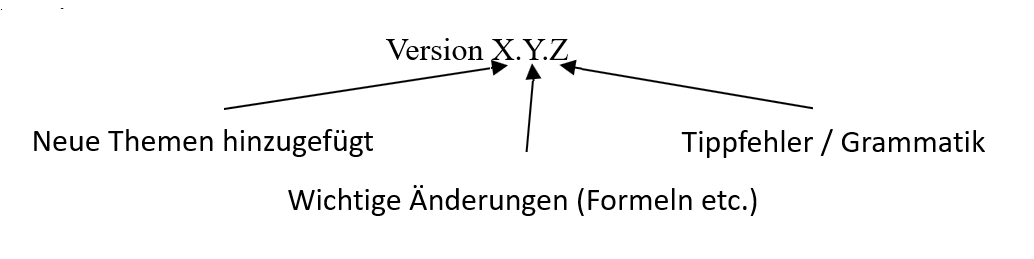
\includegraphics[scale=0.48]{img/version.png}
\end{center}


%% include the abstract without chapter number but include it on table of contents:
\cleardoublepage
\phantomsection

\tableofcontents                %% this produces the table of contents - you might have guessed :-)

\newpage
%\mainmatter                     %% KOMA: marks main part using arabic page numbers and such; only available in scrbook


\section{Mathematische Grundlagen}
\label{chap:Style}

\subsection{Koordinatensysteme}

Häufig sind wir daran interessiert, geometrische Dinge in der Mathematik darzustellen um mit ihnen zu rechnen. \\
Um mit mathematischen Mitteln geometrische Probleme beschreiben zu können, müssen wir ein System einführen, wie wir
Positionen im Raum und Richtungen charakterisieren können. \\
Zu diesem Zweck werden \textbf{Koordinatensysteme} eingeführt.

\definition{Koordinatensystem}
\beginip
Ein Koordinatensystem dient zur eindeutigen Bezeichnung der Position von Punkten in einem geometrischen Raum.  \\
Befinden wir uns in einem 3-Dimensionalem Raum so werden 3 \textbf{Basisvektoren} benötigt, um jeden Punkt im Raum eindeutig zu definieren. \\
Möchten wir nun einen Punkt im Raum beschreiben, so müssen wir zuerst einen Punkt im Raum als Bezugspunkt (Ursprung) definieren. \\
Danach beschreiben wir den gesuchten Punkt als \textbf{Linearkombination} der Basisvektoren. Die Koeffizienten der Linearkombination bezeichnen wir dabei als Koordinaten.
\iend


\bsptask{Beispiel}{Punkt im Koordinatensystem}
\beginbsp
Geben sie die Koordinaten des folgenden Punktes P im 2 Dimensionalen an. \\ Als Basisvektoren verwenden wir die Vektoren: $ \vec{e}_1, \vec{e}_2$
\begin{center}
	\ibox{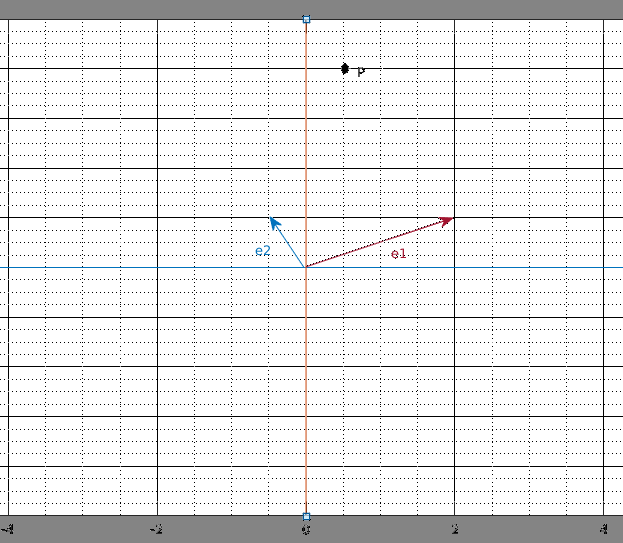
\includegraphics[scale=2.0]{img/bsp1_coord.png}}
\end{center}
\iend
\newpage
\bsp{Lösung}{}
\beginbsp
Um vom Ursprung den Punkt P mit den Basisvektoren $\vec{e}_1$ und $\vec{e}_2$ zu erreichen, müssen die Vektoren wie folgt kombiniert werden:
\begin{center}
	\ibox{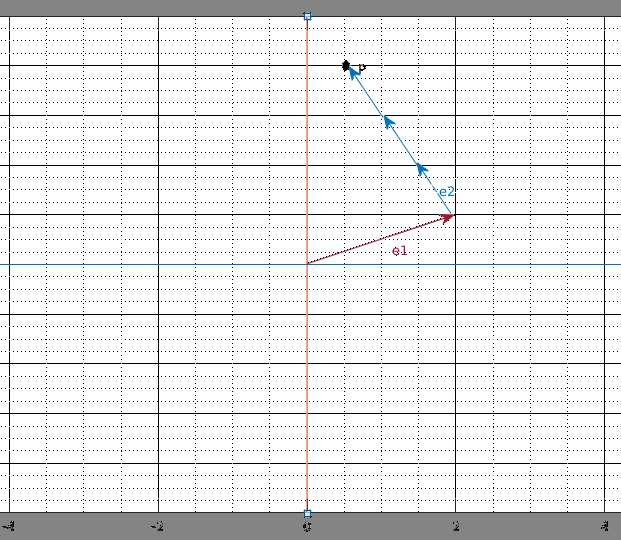
\includegraphics[scale=2.0]{img/sol_1_koord.png}}
\end{center}
Somit gilt für den Punkt P : \\
\begin{center}
	$\vec{P} = 1\cdot \vec{e}_1 + 3 \cdot \vec{e}_2$ \\
	$\rightarrow \doubleunderline{ P = \left ( \begin{array}{c} 1 \\ 3 \end{array}\right)}$
\end{center}
\iend

\newpage


\important{Konzept}{Winkelabhängige Basisvektoren *}
\beginip
In gewissen Koordinatensystemen werden Basisvektoren verwendet, dessen Richtung sich Abhängig  des Winkels ändern. \\
Sie werden dazu verwendet, Punkte im Raum abhängig eines Winkels zu beschreiben. \\
\textbf{Der Basisvektor zeigt dabei immer in die Richtung des Winkels} \\
\\
* Dies ist ein Konzept, welches Mathematisch nicht genau so existiert.
\iend

\bsptask{Beispiel}{Punkt im Koordinatensystem - Polarkoordinaten}
\beginbsp
Geben sie die Koordinaten des folgenden Punktes P im 2 Dimensionalen an.
\\
Als Basisvektoren verwenden wir die Vektoren: $ \vec{e}_1, \vec{e}_2$, wobei $\vec{e}_2$ ein Winkelabhängiger Basisvektor ist.
\begin{center}
	\ibox{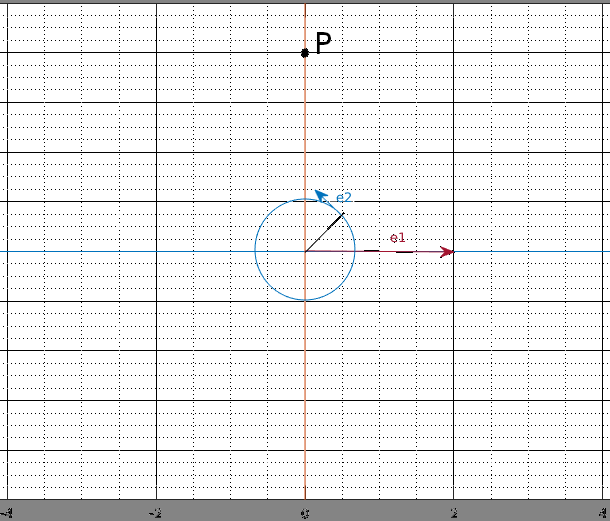
\includegraphics[scale=2.0]{img/ex2_coord.png}}

\end{center}
\iend
\bsp{Lösung}{}
\beginbsp
Da der Punkt P einen Winkel von $90^\circ = \frac{\pi}{2}$ einschliesst, müssen wir ein Winkelabhängigen Basisvektor $\vec{e}_2$ mit $\frac{\pi}{2}$ multiplizieren. \\
Der Abstand des Punktes zum Ursprung beträgt 8 Einheiten, wobei der Vektor $\vec{e}_1$ die Länge von 2 Einheiten besitzt. \\
Somit gilt für die Koordinaten des Punktes P in Abhängigkeit von $\vec{e}_1 , \vec{e}_2$:
\begin{center}
	$\vec{P} = \frac{\pi}{2} \cdot \vec{e}_2 + 4\cdot \vec{e}_1$
	\\ $\displaystyle \doubleunderline{P = \left ( \begin{array}{c} 4 \\ \frac{\pi}{2} \end{array}\right)}$
\end{center}

\iend
\newpage




\subsubsection{Kartesische Koordinaten}

\important{Kartesische Koordinaten} {}
\beginip
Kartesische Koordinaten werden als bekannt vorausgesetzt. \\
Kartesische Koord. werden vor allem dann verwendet, wenn die geometrische Anordnung \textbf{Symmetrien bezüglich einer Ebene} besitzt.
\begin{center}
	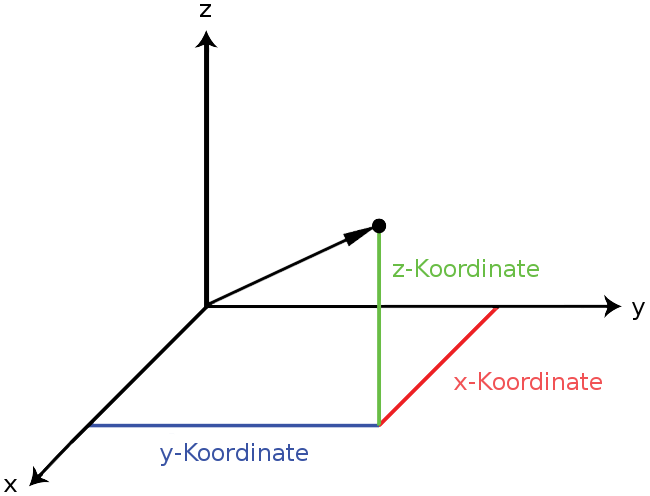
\includegraphics[scale=0.3]{img/cartesian.png}
\end{center}
\iend

\newpage
%TODO ggf. Zusammenfassung

\subsubsection{Zylinderkoordinaten}

\important{Zylinderkoordinaten} {}
\beginip
Zylinderkoordinaten werden meist dann
verwendet, wenn die geometrischen Anordnung Symmetrien bezüglich einer \textbf{Gerade} aufweist. \\
Zylinderkoordinaten besitzen 3 Basisvektoren wovon 1 winkelförmig ist. \\
\\
\textbf{Basisvektoren}
\begin{enumerate}
	\item $\vec{e}_\rho$ Beschreibt den Abstand zur Symmetrieachse
	\item $\vec{e}_\varphi$ Beschreibt den Winkel des Punktes in der XY-Ebene
	\item $\vec{e}_z$ Beschreibt den Abstand auf der Symmetrieachse
\end{enumerate}
\begin{center}
	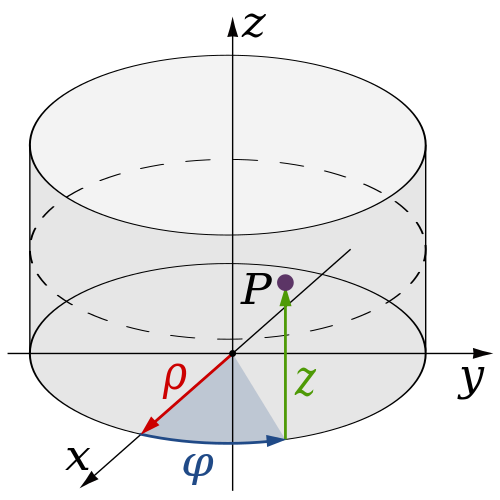
\includegraphics[scale = 0.4]{zylinderkoord.png}
\end{center}


\iend
\newpage
\important{Richtung der einzelnen Basisvektoren für beliebige Punkte im Raum: }{}


\beginip


\fboxsep=0pt
\begin{minipage}[t]{0.48\linewidth}

	\begin{center}

		\textbf{Radialer Vektor} $\vec{e}_\rho$

	\end{center}

	\begin{center}

		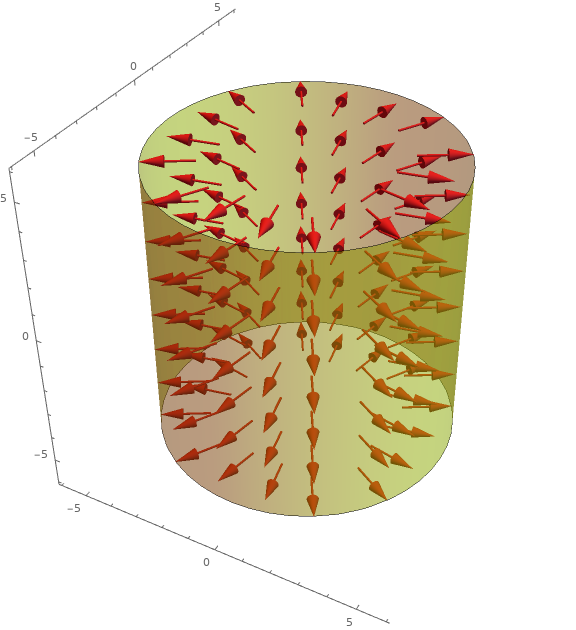
\includegraphics[scale=0.3]{zylindric_rho.png}

	\end{center}
\end{minipage}
\hfill%
\begin{minipage}[t]{0.48\linewidth}



	\begin{center}

		\textbf{Azimutaler Vektor} $\vec{e}_\varphi$

	\end{center}

	\begin{center}

		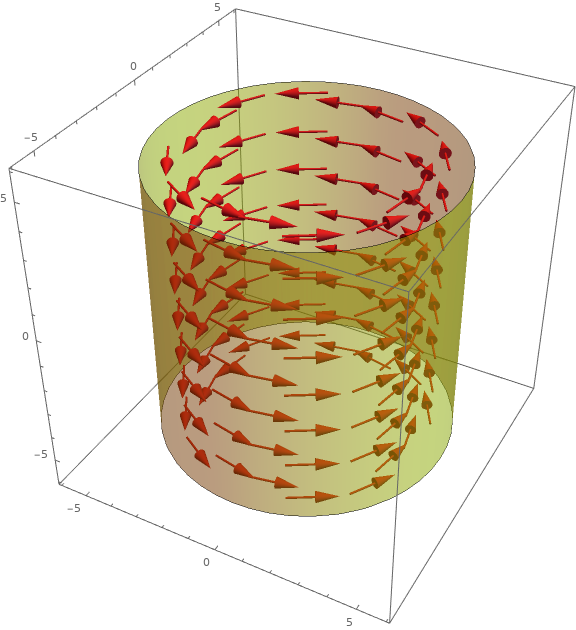
\includegraphics[scale=0.3]{zylindric_phi.png}


	\end{center}

\end{minipage}


\begin{center}

	\textbf{Abstandsvektor} $\vec{e}_z$

\end{center}

\begin{center}

	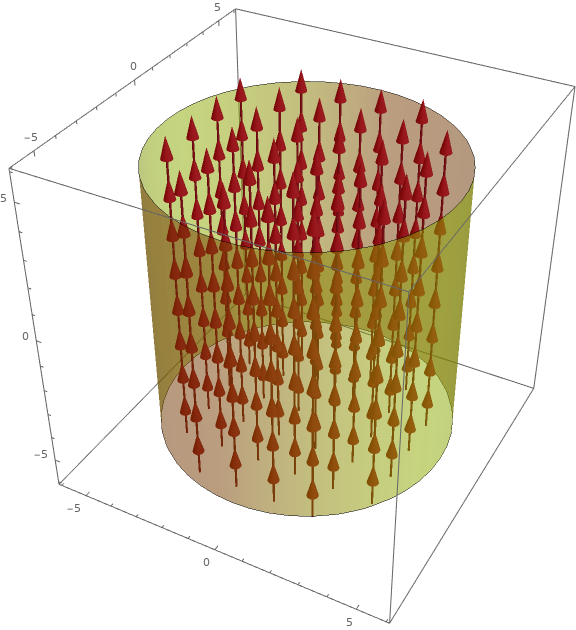
\includegraphics[scale=0.3]{zylindric_z.png}

\end{center}
\iend



\newpage

\subsubsection{Kugelkoordinaten}

\important{Kugelkoordinaten} {}
\beginip
Kugelkoordinaten werden meist dann verwendet, wenn die geometrischen Anordnung \textbf{Punktsymmetrien} aufweist. \\
Kugelkoordinaten besitzen 3 Basisvektoren wovon 2 winkelabhängig sind. \\
\\
\textbf{Basisvektoren}
\begin{enumerate}
	\item $\vec{e}_r$ Beschreibt den Abstand zum Ursprung
	\item $\vec{e}_\theta$ Beschreibt den Winkel des Punktes in der ZY-Ebene
	\item $\vec{e}_\varphi$ Beschreibt den Winkel des Punktes in der XY-Ebene
\end{enumerate}
\begin{center}
	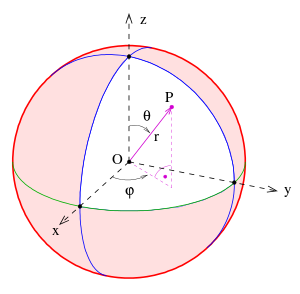
\includegraphics[scale = 0.5	]{kugelkoord.png}
\end{center}


\iend
\newpage
\important{Richtung der einzelnen Basisvektoren für beliebige Punkte im Raum: }{}


\beginip


\fboxsep=0pt
\begin{minipage}[t]{0.48\linewidth}

	\begin{center}

		\textbf{Radialer Vektor} $\vec{e}_r$

	\end{center}

	\begin{center}

		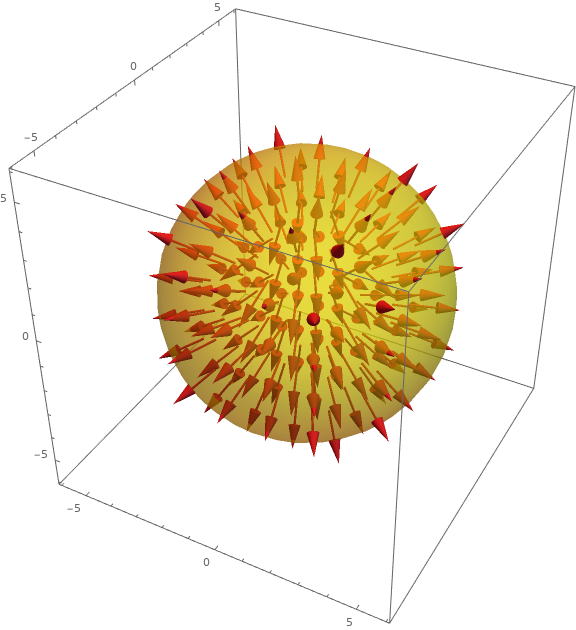
\includegraphics[scale=0.4]{spherical_r.png}

	\end{center}
\end{minipage}
\hfill%
\begin{minipage}[t]{0.48\linewidth}



	\begin{center}

		\textbf{Azimutaler Vektor} $\vec{e}_\varphi$

	\end{center}

	\begin{center}

		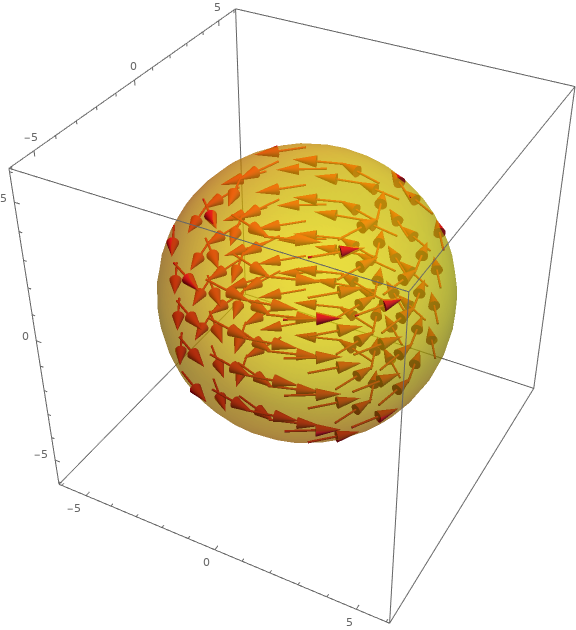
\includegraphics[scale=0.4]{spherical_phi.png}

	\end{center}

\end{minipage}


\begin{center}

	\textbf{Meridonaler Vektor} $\vec{e}_\theta$

\end{center}

\begin{center}

	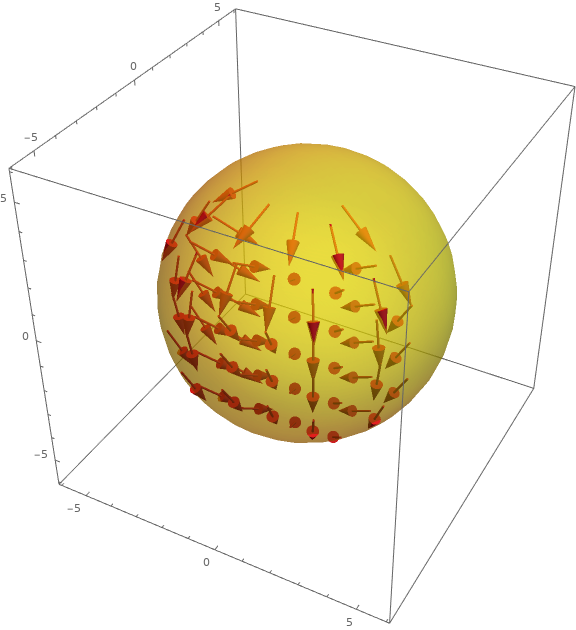
\includegraphics[scale=0.4]{spherical_theta.png}

\end{center}

% \formulaBegin
% $\displaystyle \vec{F}(r, \theta, \varphi) = \left(\begin{array}{c} 1 \\ 0 \\ 0 \end{array}\right)_{K} = 1 \cdot \vec{e}_r$ \\
%
% \formulaEnd


% \formulaBegin
% $\vec{F}(r, \theta, \varphi) = \left(\begin{array}{c} 0 \\ 1 \\ 0 \end{array}\right)_{Kugel\ Koordinaten} = 1 \cdot \vec{e}_\theta$ \\
%
% \formulaEnd

%
% \formulaBegin
% $\vec{F}(r, \theta, \varphi) = \left(\begin{array}{c} 0 \\ 0 \\ 1 \end{array}\right)_{Kugel\ Koordinaten} = 1 \cdot \vec{e}_\varphi$ \\
%
% \formulaEnd





\iend

\newpage
\subsubsection{Zusammenfassung}
\bgroup

\begin{tabular}{ c | c | c }
	Kartesische Koordinaten                                  & Zylinderkoordinaten                                         & Kugelkoordinaten                                              \\
	\hline
	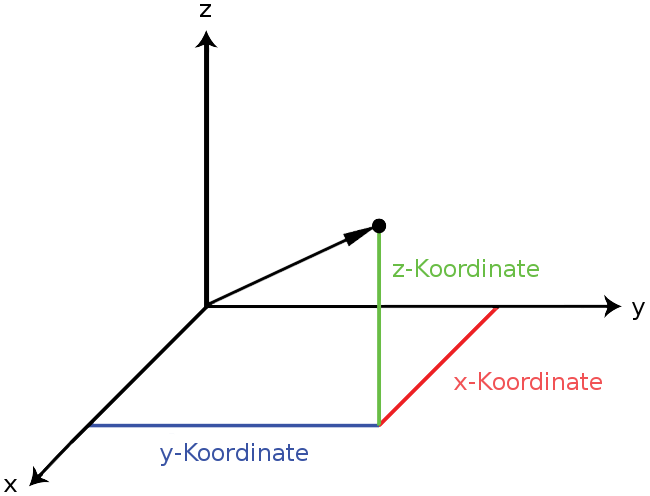
\includegraphics[width = 0.25\columnwidth]{img/cartesian.png} &
	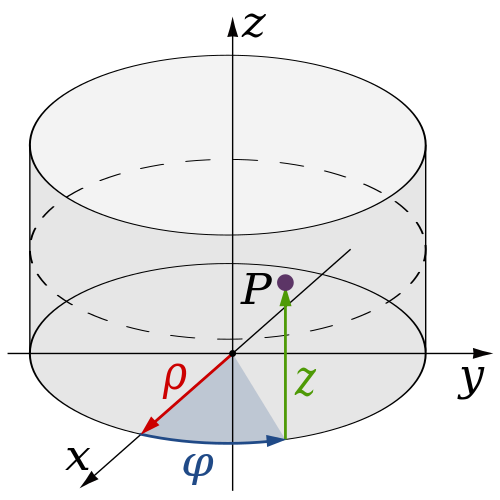
\includegraphics[width = 0.25\columnwidth]{zylinderkoord.png} &  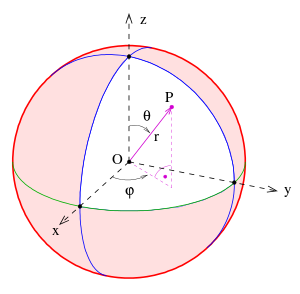
\includegraphics[width = 0.25\columnwidth]{kugelkoord.png} \\
	\hline
	\textbf{Anwenden bei:}                                   & \textbf{Anwenden bei:}                                      & \textbf{Anwenden bei:}                                        \\
	Symmetrie zu Ebene                                       & Symmetrie zu Achse                                          & Symmetrie zu Punkt                                            \\
	\hline
	$\displaystyle \left ( \begin{array}{c} x \\ y \\ z  \end{array}\right) = x \cdot \vec{e}_x + y \cdot \vec{e}_y + z \cdot \vec{e}_z$ &

	$\displaystyle \left ( \begin{array}{c} \rho \\ \varphi \\ z  \end{array}\right) = \rho \cdot \vec{e}_\rho + \varphi \cdot \vec{e}_\varphi + z \cdot \vec{e}_z$ &



	$\displaystyle \left ( \begin{array}{c} r \\ \theta \\ \varphi  \end{array}\right) = r \cdot \vec{e}_r + \theta \cdot \vec{e}_\theta + \varphi \cdot \vec{e}_\varphi $  \\
	\hline
	$\vec{e}_x$                                              & $\vec{e}_\rho$                                              & $\vec{e}_r$                                                   \\
	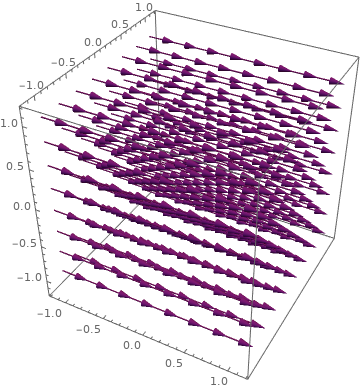
\includegraphics[width=0.25\columnwidth]{img/kart_x.png}

	&

	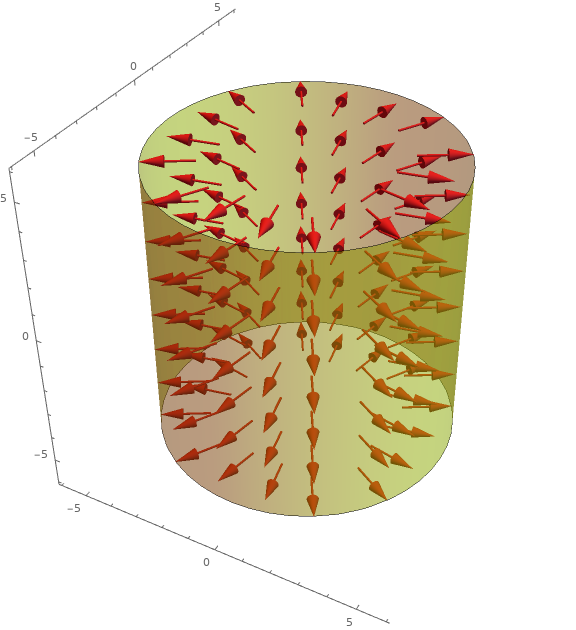
\includegraphics[width=0.25\columnwidth]{zylindric_rho.png}  & 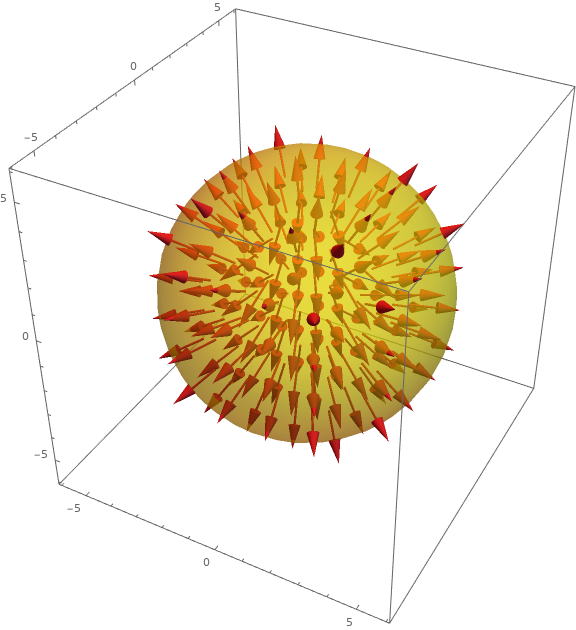
\includegraphics[width=0.25\columnwidth]{spherical_r.png} \\

	\hline
	$\vec{e}_y$                                              & $\vec{e}_\varphi$                                           & $\vec{e}_\theta$                                              \\

	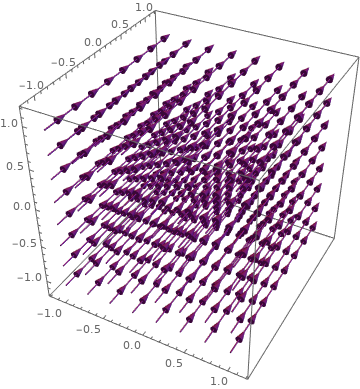
\includegraphics[width=0.25\columnwidth]{img/kart_y.png} & 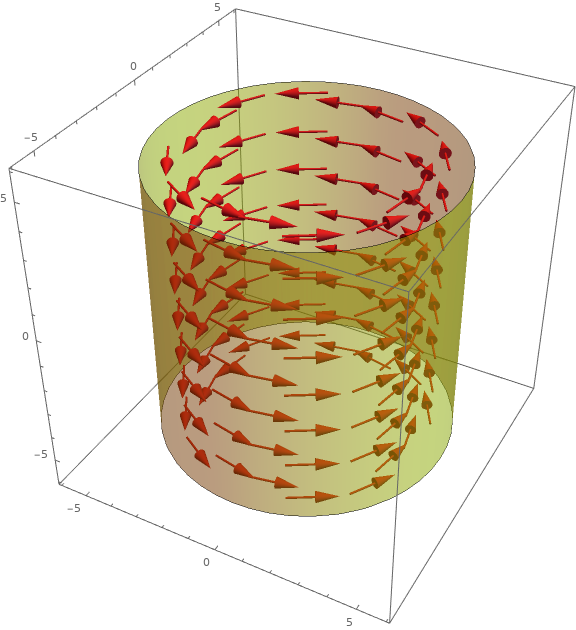
\includegraphics[width=0.25\columnwidth]{zylindric_phi.png} & 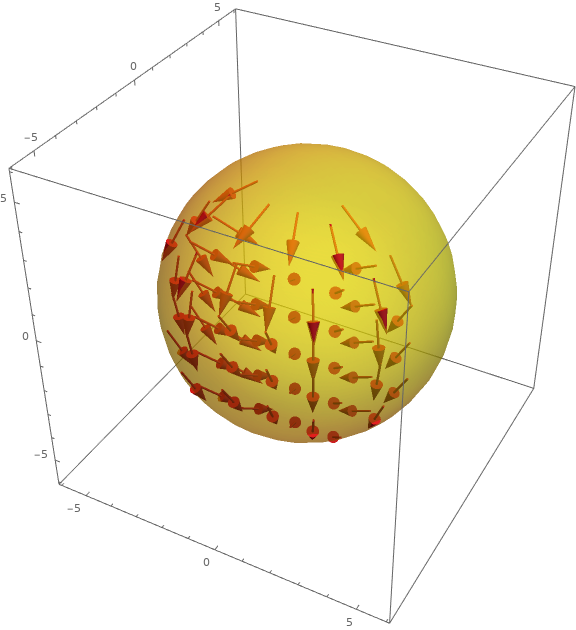
\includegraphics[width=0.25\columnwidth]{spherical_theta.png} \\
	\hline
	$\vec{e}_z$                                              & $\vec{e}_z$                                                 & $\vec{e}_\varphi$                                             \\
	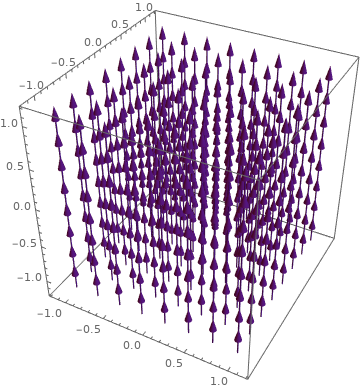
\includegraphics[width=0.25\columnwidth]{img/kart_z.png} & 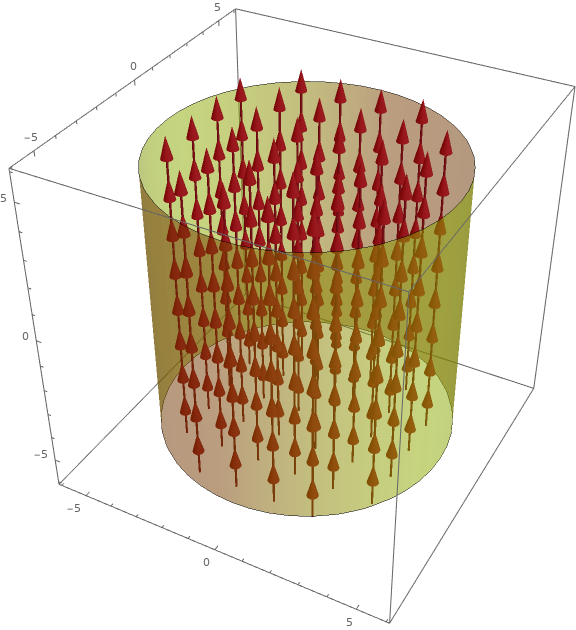
\includegraphics[width=0.25\columnwidth]{zylindric_z.png}   & 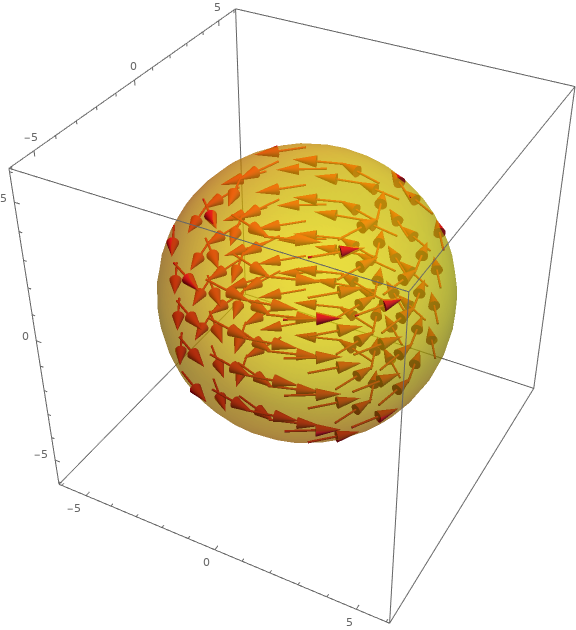
\includegraphics[width=0.25\columnwidth]{spherical_phi.png}   \\
	\hline

\end{tabular}
\egroup

\newpage






\subsection{Vektorfelder}
Möchten wir eine physikalische Grösse im Raum beschreiben, so sind wir häufig nicht nur an den ortsabhängigen Punkten interessiert. \\
Meistens möchten wir jedem Punkt im Raum eine Richtung zuordnen. \\
Möchten wir beispielsweise die Erdanziehungskraft modellieren, so wollen wir jedem Punkt im Raum einen \textbf{Vektor} zuweisen, der in Richtung der Kraftwirkung zeigt. \\
Seine Länge soll zudem die Information beinhalten, wie stark die Kraft an diesem Punkt wirkt.










%
%
%
% \formulaBegin
% $\vec{F}(\rho, \varphi, z) = \left(\begin{array}{c} 1 \\ 0 \\ 0 \end{array}\right)_{Zylinder\ Koordinaten} = 1 \cdot \vec{e}_\rho$ \\
%
% \formulaEnd
% \begin{center}
%
% 	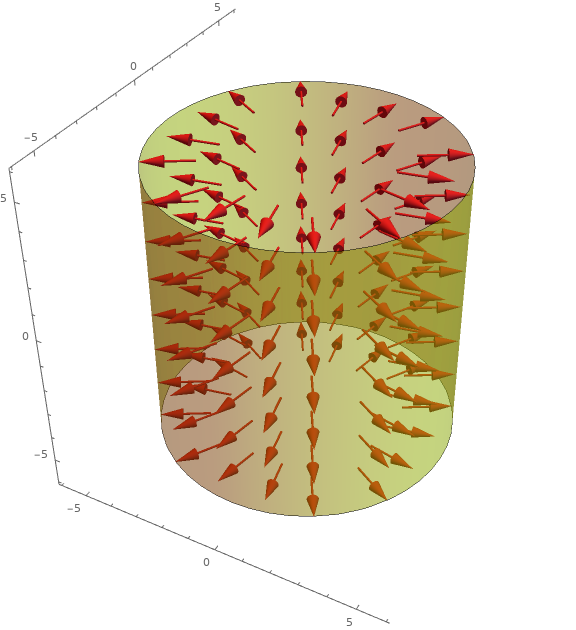
\includegraphics[scale=0.4]{zylindric_rho.png}
%
% \end{center}
%
%
% \formulaBegin
% $\vec{F}(\rho, \varphi, z) = \left(\begin{array}{c} 0 \\ 1 \\ 0 \end{array}\right)_{Zylinder\ Koordinaten} = 1 \cdot \vec{e}_\varphi$ \\
%
% \formulaEnd
% \begin{center}
%
% 	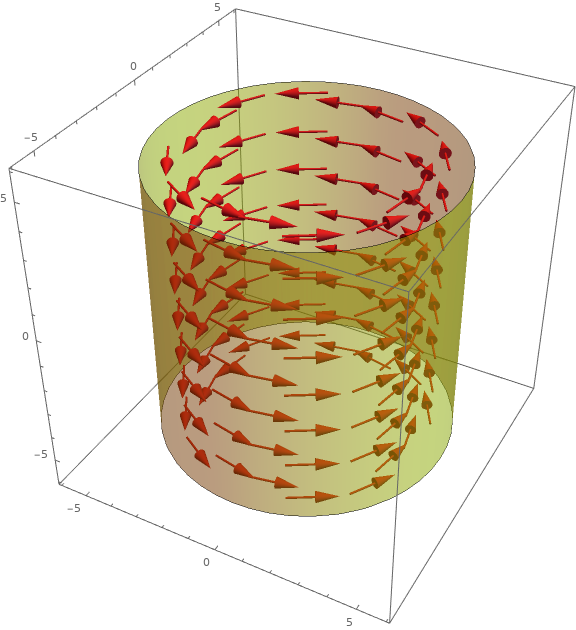
\includegraphics[scale=0.4]{zylindric_phi.png}
%
% \end{center}
%
%
%
%
% \formulaBegin
% $\vec{F}(\rho, \varphi, z) = \left(\begin{array}{c} 0 \\ 0 \\ 1 \end{array}\right)_{Zylinder\ Koordinaten} = 1 \cdot \vec{e}_z$ \\
%
% \formulaEnd
% \begin{center}
%
% 	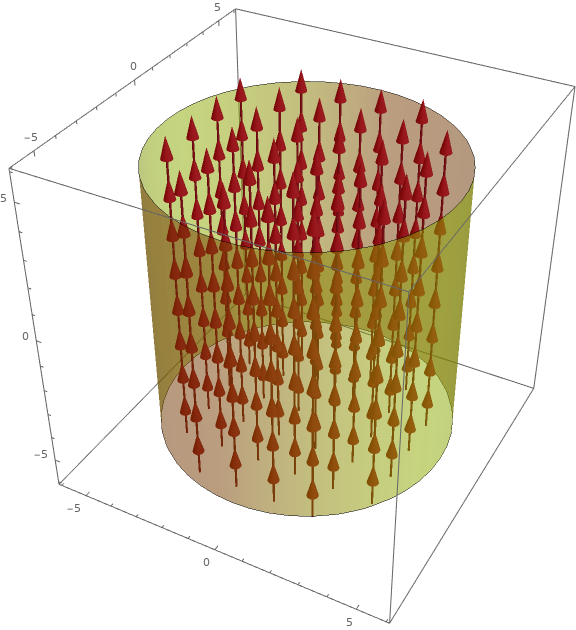
\includegraphics[scale=0.4]{zylindric_z.png}
%
% \end{center}
%
%
%
% \important{Zylinderkoordinaten} {}
% \beginip
%
% 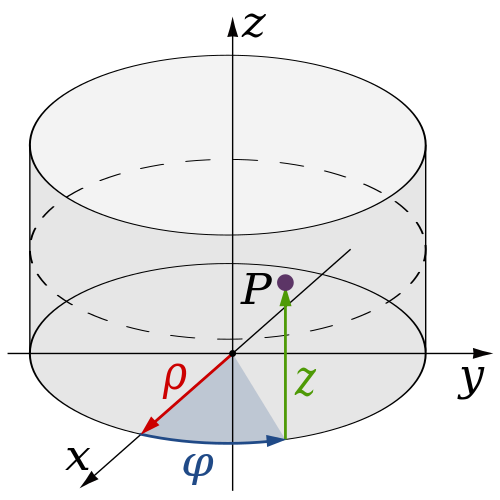
\includegraphics[scale = 0.4]{zylinderkoord.png}
% \iend
%
% \important{Kugelkoordinaten} {}
% \beginip
% \iend
%

\important{Defintion}{Vektorfeld}
\beginip
Ein Vektorfeld, bezeichnet eine mathematische Funktion, welche anstatt einer skalaren Grösse Vektoren zurück gibt. \\
Häufig ist ein Vektorfeld nicht nur von einer Variable (x) abhängig, sondern besitzt 3 Parameter (x,y,z) die wir manchmal als Ortsvektor $\vec{r}$ zusammenfassen.  \\
\iend

\bsp{Beispiel} {Vektorfeld - Gravitation}

\beginbsp
Möchten wir beispielsweise das Gravitationsfeld der Erde mathematisch beschreiben, würden wir dies in Form eines Vektorfeldes tun. \\
Dieses Vektorfeld soll jedem Punkt einen Kraftvektor zuweisen, welcher in Richtung Erdmittelpunkt zeigt. \\
Da die Erde punktsymmetrisch ist, ist es sinnvoll Kugelkoordinaten zu verwenden. \\
Die Stärke der Gravitationskraft auf ein Massepunkt der Masse m ist definiert als:
\begin{center}
	$F_M = \frac{M \cdot G}{r^2}$
\end{center}

Somit folgt für das Vektorfeld, das die Gravitationskraft beschreibt:
\begin{center}
	$\displaystyle \vec{F}_M (r,\theta,\varphi) = \frac{M \cdot G}{r^2} \cdot (- \vec{e}_r)$
\end{center}

\begin{center}
	\ibox{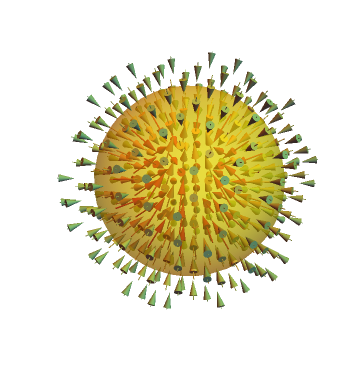
\includegraphics[scale=0.4]{img/vektorfeld-g.png}}

\end{center}
\iend

\newpage
\subsection{Weg- und Oberflächenintegrale}

\gl{Gleichung}{Wegintegral über ein Vektorfeld}
\begingl
Wegintegrale beschreiben die Auswirkungen eines Vektorfeldes auf ein Teilchen, welches sich entlang eines Weges bewegt. \\
Sie können in unserem Fall, häufig als ein Mass der Arbeit, welche aufgewendet werden muss, um ein Teilchen von A nach B zu bewegen, aufgefasst werden. \\

Wir notieren das Wegintegral über einen Weg $\gamma$ folgendermassen: \\
\formulaBegin
$ \displaystyle \int_\gamma \vec{E} \cdot d\vec{s}$
\formulaEnd

Können wir den Weg $\gamma$ als mathematische Funktion von t ausdrücken, so lässt sich das Integral folgendermassen darstellen:
\formulaBegin
$\displaystyle \int_{t_0}^{t_e} \vec{E}(\gamma(t)) \cdot \dot{\vec{\gamma}}(t) \cdot dt$
\formulaEnd
\textbf{Variablen} \\
$\gamma(t_0) = $ Startpunkt ,  $\gamma(t_e) = $ Endpunkt , $ \dot{\vec{\gamma}}(t) = $ Zeitliche Ableitung der Kurve \\


Das Integral selbst ist relativ schwer zu rechnen. Häufig lässt es sich jedoch vereinfachen:
Ist der Weg \textbf{parallel zur Richtung des Feldes}, so vereinfacht sich das Integral über eine vektorielle Grösse zu einem Integral über eine skalare Grösse \\
\formulaBegin
$\displaystyle \int_\gamma \vec{E} \cdot d\vec{s} = \int_A^B E(r) \cdot dr $
\formulaEnd
\textbf{Variablen} \\
$ A  = $ Startpunkt des Weges\\
$ B = $ Endpunkt des Weges \\

Für den Fall, dass das Feld auf dem \textbf{gesamten Weg konstant} ist, lässt es sich noch weiter vereinfachen: \\
\formulaBegin
$\displaystyle \int_\gamma \vec{E} \cdot d\vec{s} = l_{AB} \cdot |\vec{E}|$
\formulaEnd
\textbf{Variablen} \\
$ l_{AB}  = $ Länge des Weges im Feld\\
Ist das Feld konstant, schliesst aber mit dem Weg \textbf{immer einen Winkel} $\varphi$ ein, so gilt für das Integral: \\
\formulaBegin
$\displaystyle \int_\gamma \vec{E} \cdot d\vec{s} = l_{AB} \cdot |\vec{E}|\cdot cos(\varphi)$
\formulaEnd
\textbf{Variablen} \\
$ \varphi  = $  Winkel zwischen Wegrichtung und Richtung des Feldes\\

\iend
\important{Begründung}{Wegintegral}
\beginip
Wir betrachten ein Vektorfeld $\vec{H} = H \cdot \vec{e}_H$  (Grün) und ein Weg $\vec{s} = s \cdot \vec{e}_s$ (Blau). \\
Wir interessieren uns dafür, wie viel Arbeit wir aufwenden müssen, um uns von Punkt A (unten Links) nach Punkt B (oben Rechts) zu bewegen. \\
Wir gehen nun davon aus, dass auf einem sehr kleinem Wegstück $\Delta s$ sich die Richtung und Stärke des Feldes nicht ändert, sowie die Richtung des Weges gleich bleibt.
\ibox{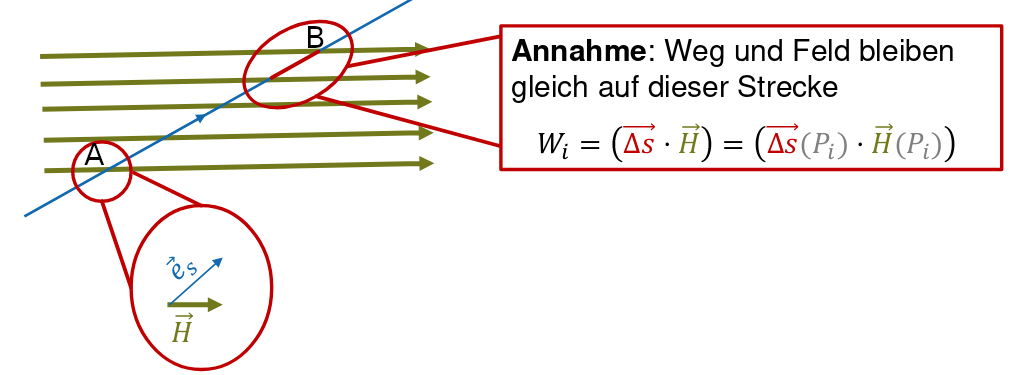
\includegraphics[scale=1.5]{img/wegintegral_beg.png}}
Die Arbeit $W_i$ bezeichnen wir als die Arbeit, welche wir aufwenden müssen, um uns auf dem Weg $\gamma$ um ein Stück $\Delta s$ nach Vorne zu bewegen. \\
Diese Arbeit ist Abhängig davon, wie Weg und Feld geometrisch stehen. Möchten wir uns senkrecht zum Feld bewegen, so wirkt nichts dieser Bewegungsrichtung entgegen und die  Arbeit ist gleich 0. \\
Möchten wir uns hingegen parallel zum E-Feld bewegen, so müssen wir maximale Arbeit verrichten, da das E-Feld uns maximal beeinflusst. \\
\\
Den Winkel, welcher das Feld mit dem Weg einschliesst, ist gegeben als $ cos(\varphi) = \vec{e}_s \cdot \vec{e}_H$. \\
Somit gilt für die Arbeit, welche auf dem Weg $\Delta s$ aufgewendet wird: $W_i = |H(P_i)| \cdot \Delta s \cdot  \vec{e}_s \cdot \vec{e}_H = \vec{H}(P_i) \cdot \Delta \vec{s}(P_i)$ \\
Für den gesamten Weg gilt somit:
$\displaystyle W_{ges} = \sum_i W_i = \sum_i \vec{e}_H = \vec{H}(P_i) \cdot \Delta \vec{s}(P_i) \Rightarrow i\rightarrow \infty $

\begin{center}
	$ W_{ges} = \int_A^B \vec{H}(\vec{P})\cdot d\vec{s} $
\end{center}
Ist der Weg s als Funktion gegeben, mit $s(t_0) = A $ und $s(t_e) = B$, so gilt für den Punkt P: $\vec{P} = \vec{s}(t)$ und den kleinen Richtungsvektor $ d\vec{s}$  des Weges: \\


\fboxsep=0pt
\begin{minipage}[t]{0.68\linewidth}

	\begin{flushright}
		$ \vec{s}(t) = \left(\begin{array}{c} f_1(t) \\ f_2(t)  \end{array}\right)$ \\
		\fspace
		$ \displaystyle \frac{d}{dt}(\vec{s}(t)) = \dot{\vec{s}}(t) $ \\
		\fspace
		$ \displaystyle d\vec{s}(t) = \dot{\vec{s}}(t) \cdot dt = \left(\begin{array}{c} \dot{f}_1(t) \\ \dot{f}_2(t)  \end{array}\right) \cdot dt	$
	\end{flushright}
\end{minipage}
\hfill%
\begin{minipage}[t]{0.28\linewidth}
	\begin{flushleft}
		$ \displaystyle \big | \ \ \  \frac{d}{dt} \big ( . \big ) $ \\

		\fspace
		\fspace
		\fspace
		$\displaystyle  \big |\ \  \cdot dt$ \\

	\end{flushleft}
\end{minipage}


\begin{center}

\end{center}



Und somit für das gesamte Integral: \\
\begin{center}
	$ \displaystyle \int_A^B \vec{H}(\vec{P})\cdot d\vec{s} = \int_{t_0}^{t_e} \vec{H}(\vec{s(t)})\cdot \dot{\vec{s}}(t) \cdot dt $
\end{center}
\iend


\bsptask{Beispiel}{Wegintegral über ein Vektorfeld}
\beginbsp
Gegeben sei das Vektorfeld in den Kartesischen Koordinaten $\vec{E}(x,y,z) =  \left(\begin{array}{c} x + 2y \\ 5z\\ x\\ \end{array}\right) $ \\
Berechnen sie das Wegintegral, über eine Gerade vom Punkt $\left(\begin{array}{c} 0 \\ 0\\ 0\\ \end{array}\right)$ zu $\left(\begin{array}{c} 5 \\ 2\\ 1\\ \end{array}\right)$
\iend

\vspace \fill

\bsp{Lösung}{}
\beginbsp
Zuerst müssen wir die Gerade vom Punkt $(0,0,0)$ zu $(5,2,1)$ als Funktion parameterisieren. \\
Aus der Vektorrechnung folgt für die Geradengleichung:
\begin{center}
	$\gamma(t) = \left(\begin{array}{c} 0 \\ 0\\ 0\\ \end{array}\right)  +  \left(\begin{array}{c} 5 \\ 2\\ 1\\ \end{array}\right) \cdot t = \left(\begin{array}{c} x \\ y\\ z\\ \end{array}\right)$
\end{center}
Somit gelten für Anfang und Endpunkte unserer Kurve:
\begin{center}
	$A = (0,0,0)^T = \gamma(0) \rightarrow t_0 = 0$ \\
	$B = (5,2,1)^T = \gamma(1) \rightarrow t_e = 1$
\end{center}

Für $d\vec{\gamma}$ folgt:
\begin{center}
	$ \displaystyle d\vec{\gamma} = \dot{\gamma} \cdot dt = \left(\begin{array}{c} \frac{d}{dt}(5 \cdot t) \\ \frac{d}{dt}(2 \cdot t)\\ \frac{d}{dt}(1 \cdot t)\\ \end{array}\right) \cdot dt = \left(\begin{array}{c} 5 \\ 2\\ 1\\ \end{array}\right) \cdot dt$
\end{center}

Und für $\vec{E}(\vec{\gamma}(t))$ :
\begin{center}
	$\vec{P} = \vec{\gamma(t)} =  \left(\begin{array}{c} 5t \\ 2t\\ 1t\\ \end{array}\right) = \left(\begin{array}{c} x \\ y\\ z\\\end{array}\right)$ \\
	$\Rightarrow \vec{E}(\vec{P}) =  \left(\begin{array}{c} 5t + 2\cdot2t \\ 5\cdot 1t\\ 5t\\ \end{array}\right) =  \left(\begin{array}{c} 9t \\ 5t\\ 5t\\ \end{array}\right) $ \
\end{center}
Somit folgt für das Integral:
\begin{center}
	$\displaystyle \doubleunderline{\int_\gamma \vec{E}\cdot d\vec{\gamma}} =  \int_0^1 \left(\begin{array}{c} 9t \\ 5t\\ 5t\\ \end{array}\right)  \cdot \left(\begin{array}{c} 5 \\ 2\\ 1\\ \end{array}\right)\cdot dt = \int_0^1 45t + 10t + 5t \cdot dt = \int_0^1 60t \cdot dt = \doubleunderline{30} $
\end{center}

\iend

\newpage

\bsptask{Beispiel}{Wegintegral in Kugelkoordinaten}
\beginbsp
Gegeben sei das Vektorfeld in Kugelkoordinaten $\vec{E}(r,\theta,\varphi) =  \left(\begin{array}{c} 5 \cdot r^2 \\ 0 \\ 0 \end{array}\right) = 5 \cdot r^2\cdot \vec{e}_r$ \\
Berechnen sie das Wegintegral, über eine Gerade (in Kugelkoordinaten) vom Punkt $\left(\begin{array}{c} 0 \\ 0\\ 0\\ \end{array}\right)$ zu $\left(\begin{array}{c} 5 \\ 0\\ 0 \\ \end{array}\right)$

\iend


%\vspace \vfill
\bsp{Lösung}{}
\beginbsp
\textbf{Intuitive Lösung:} \\
Da der Weg parallel zum Feld ist ($\vec{e}_\gamma = \vec{e}_E$) vereinfacht sich das Wegintegral zu einem Skalaren Integral:
\begin{center}
	$\displaystyle \int_\gamma \vec{E}\cdot d\vec{\gamma} = \int_0^5 5 \cdot r^2 dr = \frac{1}{3} \cdot 5 \cdot 125 = \frac{625}{3}$
\end{center}
\textbf{Mathematische Lösung} \\
Wir beschreiben die Kurve $\gamma$ in Kugelkoordinaten:
\begin{center}
	$\gamma(t) = 5 \cdot t \cdot \vec{e}_r$
\end{center}
Somit folgt für $d \vec{\gamma}$
\begin{center}
	$d \vec{\gamma} = 5\cdot \vec{e}_r \cdot dt$
\end{center}
Und für das Integral:
\begin{center}

	$\displaystyle \int_\gamma \vec{E}\cdot d\vec{\gamma} =\int_0^1 \vec{E} \cdot 5 \cdot \vec{e}_r =  \int_0^1 5 \cdot (5t)^2 \cdot \vec{e_r} \cdot 5 \cdot \vec{e}_r dt =  \int_0^1 5^4 \cdot t^2 dt = \frac{1}{3} \cdot 5 \cdot 125 = \frac{625}{3}$
\end{center}
\iend

\newpage

\gl{Gleichung}{Fluss eines Vektorfeldes}
\begingl
Die folgende Gleichung bezeichnen wir als Oberflächenintegral des Vektorfeldes $\vec{E}$. \\
Der Wert des Integrales gibt uns eine Information darüber, wieviel Feld durch eine gegebene Hüllfäche "fliesst" \\

\formulaBegin
$ \displaystyle \Phi = \oiint_A \vec{E} \cdot d\vec{A}$
\formulaEnd
\textbf{Variablen} \\
$\vec{E} =$ ein Vektorfeld\\
$A = $ Fläche, welche geschlossen ist\\
$\vec{A} =$ Normalenvektor der Fläche \\
\\

Das Integral selbst ist relativ schwer zu rechnen. Häufig lässt es sich jedoch vereinfachen:
Steht das Vektorfeld \textbf{senkrecht} zur Hüllfläche und ist es auf der gesamten Fläche \textbf{konstant}, so gilt für das Integral: \\

\formulaBegin
$ \displaystyle \oiint_A \vec{E} \cdot d\vec{A} = \pm A_{eff} \cdot |\vec{E}|$
\formulaEnd
\textbf{Variablen} \\
$A_{eff} =$ Die Fläche auf der das Feld ungleich 0 ist\\


Ist das Feld zwar konstant auf der gesamten Fläche, fliesst jedoch \textbf{nicht senkrecht} hindurch, so lässt sich das Integral auch zu einer Multiplikation vereinfachen:
\begin{center}
	\ibox{\includegraphics[scale=0.4]{img/vektorfIeld_oi.png}}
\end{center}
\formulaBegin
$ \displaystyle \oiint_A \vec{E} \cdot d\vec{A} = \pm A_{eff} \cdot |\vec{E}| \cdot cos(\varphi)$
\formulaEnd

\textbf{Variablen} \\
$\varphi =$ Winkel zwischen Vektorfeld und Flächennormale\\
\iend


\newpage


\bsptask{Beispiel}{}
\beginbsp
Wir betrachten ein Rohr der Länge L und mit Radius R. \\
In der Mitte des Rohres im Ursprung des Koordinatensystems befindet sich eine Wasserquelle, welche eine gewisse Menge Wasser generiert. \\
Die Flussdichte des Wassers, ist durch folgendes Vektorfeld gegeben: \\
\begin{center}

	$\displaystyle  \vec{J}_{wasser}(x,y,z) = \left\{
	\begin{array}{@{}l@{\thinspace}l}
		1 \cdot \vec{e}_y  \cdot [\frac{L}{s \cdot m^2}]  & :  (x^2 + z^2) \leq R, y > 0    \\
		-1 \cdot \vec{e}_y  \cdot [\frac{L}{s \cdot m^2}] & :  (x^2 + z^2) \leq R, y \leq 0 \\
		0 \cdot \vec{e}_y  \cdot [\frac{L}{s \cdot m^2}]  & : sonst                         \\
	\end{array}
	\right ) $
\end{center}

\begin{enumerate}
	\item  Zeichne das Vektorfeld in einem 3-Dimensionalen Koordinatensystem. \\
	\item Berechne sie das Oberflächenintegral $ \oiint_A \vec{J} \cdot d\vec{A}$ nach aussen, wobei A die Oberfläche des Rohres mit den beiden Kreisen am Ende bezeichne.
\end{enumerate}
\iend

\newpage

\bsp{Lösung}{}
\beginbsp
\begin{enumerate}
	\item  \
	      \begin{center}

	      	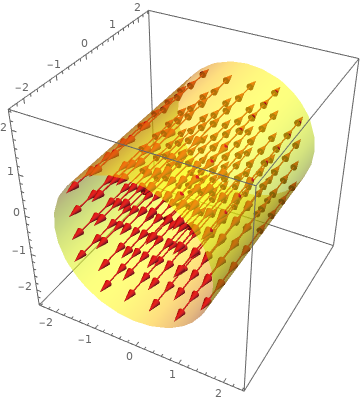
\includegraphics[scale=0.4]{plot.png}
	      	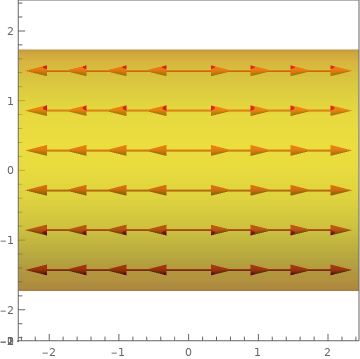
\includegraphics[scale=0.3]{plot2.png}

	      \end{center}
	\item \textbf{Intuitiver Weg} \\
	      Da das Vektorfeld nur auf den Kreisflächen ungleich Null ist, müssen wir nur das Oberflächenintegral über diese Kreisflächen berechnen. \\
	      Da das Vektorfeld auf den Kreisflächen senkrecht steht und konstant ist, vereinfacht sich dieses Integral zu einer Multiplikation mit der Fläche: \\
	      \begin{center}
	      	$\oiint_A \vec{J} \cdot d\vec{A} = A_{eff} \cdot |\vec{J}| = 2 \cdot (\pi R^2) \cdot 1 =  \doubleunderline{2\pi R^2}$
	      \end{center}



	      \textbf{Mathematischer Weg} \\ \begin{center}
	      $\oiint_A \vec{J} \cdot d\vec{A} = \iint_{Mantel} 0 \cdot d\vec{A} + \iint_{Kreise} \vec{J} d\vec{A}$ \\
	\end{center}

	Wir bezeichnen nun mit $K_1$ die erste Kreisfläche des Zylinders bei $y = - \frac{L}{2}$ und mit $K_2$ die zweite Kreisfläche bei $y = \frac{L}{2}$. Somit folgt für das Integral:
	\begin{center}
		$\oiint_A \vec{J} \cdot d\vec{A} =  \iint_{K1} -1 \vec{e_y} \cdot  d\vec{A} + \iint_{K2} 1 \vec{e_y} \cdot d\vec{A}$
	\end{center}
	Die Flächennormalen auf der ersten Kreisfläche zeigt nach $(-e_y)$, die der 2. Kreisfläche nach $(e_y)$:
	\begin{center}
		$K_1$: $ d\vec{A} = (-\vec{e}_y) \cdot dA$, $K_2$: $ d\vec{A} = \vec{e}_y \cdot dA$ \\
		$ \rightarrow  \oiint_A \vec{J} \cdot d\vec{A} =  \iint_{K_1} -1 \vec{e_y} \cdot (- \vec{e_y})  dA + \iint_{K_2} 1 \vec{e_y} \cdot \vec{e_y} dA $ \\
		$ = 1\cdot \iint_{K_1} dA + 1\cdot \iint_{K_2} dA = \pi\cdot R^2 + \pi\cdot R^2 = 2 \cdot \pi\cdot R^2$

	\end{center}

\end{enumerate}

\iend

\newpage
%----------------------------------------------------------------
%
%  File    :  thesis-style.tex
%
%  Author  :  Keith Andrews, IICM, TU Graz, Austria
%
%  Created :  27 May 93
%
%  Changed :  19 Feb 2004
%
% styling and technical implementation adopted 2011 by Karl Voit
%----------------------------------------------------------------

					\section{Elektrostatik}
					\label{chap:Style}


					Elektrisch geladene Teilchen, welche sich in der Nähe eines anderen, geladenen Teilchen befinden, verspüren eine Kraftwirkung, die Abhängig der eigenen Ladung ist. \\
					Um diese Kraftwirkung zu beschreiben, wurde der Begriff des \textbf{Elektrischen Feldes} eingeführt.

					\definition{Elektrisches Feld}
					\beginip
					Das Elektrische Feld, beschreibt die Kraftwirkung auf geladene Teilchen im Raum. \\
					Es ordnet jedem Punkt im Raum einen Vektor $\vec{E}$ zu, der in die Richtung der Kraftwirkung zeigt.
					Für die Kraftwirkung auf ein Teilchen mit der Ladung Q und dem Ortsvektor $\vec{r}$ gilt: \\
					\formulaBegin
						$\vec{F} = Q \cdot \vec{E}(\vec{r})$
					\formulaEnd
					\iend


					\textbf{Einige wichtige Felder}
					\bsp{Beispiel}{E-Feld einer Punktladung}
					\beginbsp
					Das Elektrische Feld einer Punk	tladung Q ist gegeben als:
					\formulaBegin
						$\vec{E} = \frac{1}{4 \pi \epsilon} \cdot \frac{Q}{r^2}\cdot \vec{e}_r$
					\formulaEnd
					\begin{center}
						\ibox{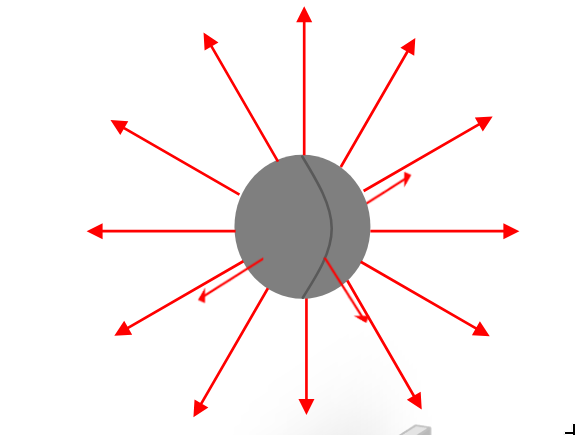
\includegraphics[scale=0.2]{img/e-feld-pkt.png}}
					\end{center}
					\iend




					\bsp{Beispiel}{E-Feld einer Platte}
					\beginbsp
					Das Elektrische Feld einer Platte mit Ladung Q ist gegeben als:
					\formulaBegin
						$\vec{E} = \begin{cases}
      \frac{Q}{2\cdot A \varepsilon} \cdot \vec{e}_n & , y > y_0 \\
			\frac{-Q}{2\cdot A \varepsilon} \cdot \vec{e}_n & , y <= y_0 \\

	 \end{cases}
$
					\formulaEnd
					\begin{center}
						\ibox{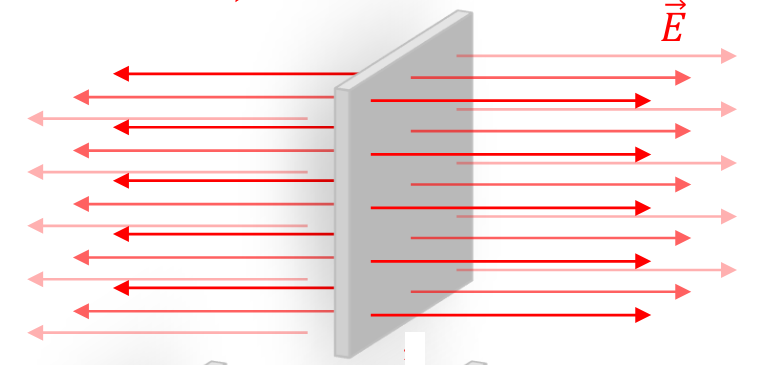
\includegraphics[scale=0.2]{img/e-feld-platte.png}}
					\end{center}
					\iend



					\bsp{Beispiel}{E-Feld eines Kondensators}
					\beginbsp
					Das Elektrische Feld in einem Kondensator mit Der Ladung Q oder Spannung U ist gegeben als:
					\formulaBegin
						$\vec{E} = \frac{Q}{A\varepsilon} \cdot \vec{e}_d = \frac{U}{d	} \vec{e}_d$
					\formulaEnd
					\begin{center}
						\ibox{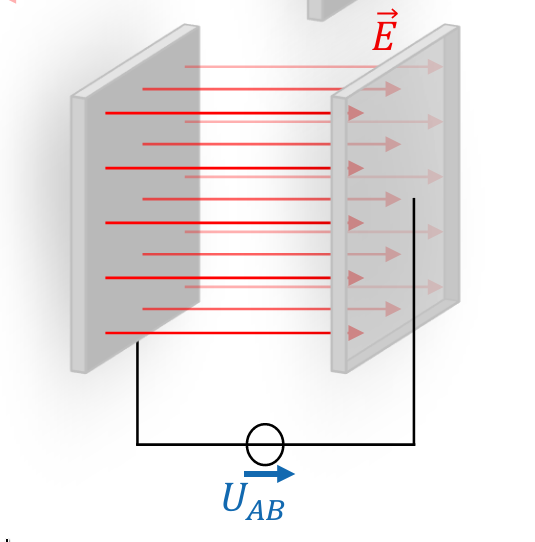
\includegraphics[scale=0.2]{img/e-feld-kond.png}}
					\end{center}
					\iend



					\subsection{(Ladungs)-Dichte}
					TODO


					\subsection{Elektrische Flussdichte}
					Quelle des Elektrischen Feldes sind geladene Teilchen. Jedoch hängt das Elektrische Feld davon ab, in was für einem Material wir uns befinden. \\
					Das Elektrische Feld in einem Metall ist zum Beispiel kleiener, als das Elektrische Feld im Vakuum. \\
					Grund dafür ist die \textbf{elektrische Influenz}, welche das Ursprüngliche Feld abschwächt) \\
					Um gewisse Rechnungen zu vereinfachen, definieren wir ein neues Feld.

					\important{Definition}{Die Elektrische Flussdichte}
					\beginip
					Die elektrische Flussdichte $\vec{D}$ beschreibt das Feld, welches existieren würde, falls kein Material vorhanden wäre.
					\iend

					Da die elektrische Flussdichte  $\vec{D}$ unabhängig vom Material ist und aussschliesslich von den Ladungsträger abhängig ist,
					gibt es eine Formel, die die beiden Grössen in Verbindung bringt:
					\gl{Gleichung}{Quellgleichung des elektrischen Flusses}

					\begingl
					\begin{center}
						\formulaBegin
						$\Psi := \oiint \vec{D}\cdot d\vec{A} = Q_{eff}$
						\formulaEnd

						Falls Feld senkrecht auf Fläche und Konstant \\
						\fspace

							\formulaBegin
							$D = |\frac{Q_{eff}}{A_{eff}}|$
							\formulaEnd

						\end{center}
						\textbf{Variabeln}: \\
						$\Psi = $ Elektrischer Fluss $ [\Psi] = A \cdot s $ \\
						$D = $ Elektrische Flussdichte $ [D] = \frac{As}{m^2}$ \\
						$ Q_{eff} = $ Von der Fläche eingeschlossene Ladung $[Q] = A\cdot s$ \\
						$ A_{eff} = $ Fläche, durch die das D-Feld durchfliesst$ [A] = m^2$ \\

					\iend

					\bsptask{Beispiel}{Berechnung des D-Feldes einer Kugel}
					\beginbsp
					Eine Kugel sei mit der Ladung $20 C$ gefüllt. Die Kugel habe den Radius $R = 2cm$ und alle Ladungsträger verteilen sich auf der Kugeloberfläche. \\
					Berechne das $\vec{D}$-Feld der Kugel.
					\iend

					\important{Lösung}{}
					\beginbsp
					Um das D-Feld der Kugel anzugeben, müssen wir zuerst ein passendes Koordinatesystem wählen. \\
					Da wir mit einer Kugel rechnen, muss das Feld Punktsymmetrisch sein und einzig der Abstand zum Kugelmittelpunkt bestimmt wie gross das D-Feld ist. \\
					Aufgrund dieser Überlegung, werden wir \textbf{Kugelkoordinaten} verwenden. (Hätten wir etwas, das Symmetrisch zur Z-Achse ist, so würden wir Zylinderkoord. verwenden etc.). \\
					Um die Gleichung für den Elektrischen Fluss anwenden zu können, müssen wir eine Hüllfläche finden,   \textbf{auf der das D-Feld Konstant ist}. \\
					Da die Anordnung eine Kugel ist, verwenden wir als Hüllfläche eine Kugel mit radius r. \\
					Nun können wir die Quellgleichung verwenden:
					\begin{center}
						$ \oiint_A \vec{D}\cdot d\vec{A} = Q_{eff} \rightarrow D \cdot  4\pi r^2  = Q_{eff} $
					\end{center}
					Der Betrag des D-Feldes entspricht also gerade der von der Hullfläche eingeschlossenen Ladung geteilt durch die Fläche. \\
					Für den Fall, dass wir die Hüllfläche grösser als die Kugel wählen, schliessen wir alle Ladungen ein: \\
					$\mathbf{r > R}$ \\
					\begin{center}
						$Q_eff = 20C$ \\
						$D = \frac{20C}{4\pi r^2}$ \\
						$\vec{D} = D \cdot \vec{e}_r$
					\end{center}

					Falls unsere Hüllfläche im inneren der Kugel ist, so schliessen wir keine Ladung ein: \\
					$\mathbf{r < R}$ \\
					\begin{center}
						$Q_eff = 0C$ \\
						$\vec{D} = 0$
					\end{center}

					Somit gilt für das D-Feld einer Kugel mit Ladungen auf der Oberfläche: \\
\begin{center}

					$
					\vec{D}(r) =
					\begin{cases}
      0 & r < R \\
      \frac{20 C}{4 \pi r^2} \cdot  \vec{e}_r & r > R \\
   \end{cases}$

	 \end{center}
					\iend




					Da die elektrische Flussdichte nur von den Ladungsträgern abhängig ist, lässt sie sich realtiv einfach berechnen und bildet meist den Grundstein für
					das Berechnen von E-Feldern usw. \\
					\" Fliesst \" eine elektrische Flussdichte durch ein Material mit Ladungsträgern, so wird diese abgeschwächt, da sich im inneren des Materiales ein
					elektrisches Feld entgegen dem von Aussen angelegtem Feld ausbildet. \\
					\includegraphics[scale=1]{todo-perm.png}

					\gl{Gleichung}{Zusammenhang E-Feld und D-Feld}
					\begingl
					\begin{center}
						\formulaBegin
						$ \vec{E} = \frac{1}{\varepsilon_0 \cdot \varepsilon_r} \cdot \vec{D}$
						\formulaEnd
					\end{center}
					\textbf{Variabeln}: \\
					$D = $ Elektrische Flussdichte $ [D] = \frac{As}{m^2}$ \\
					$ E = $ Elektrisches Felder $[E] = \frac{V}{m}$ \\
					$ \varepsilon_0 = $ Dielektrizitätskonstante $ [\varepsilon_0] = \frac{C}{V\cdot m}$ \\
					$ \varepsilon_r = $ rel. Permitivität. Unterschiedlich im Material $ [\varepsilon_r] = [ ]$ \\

					\iend



					\Definition{Verhalten von Feldgrössen bei Materialübergängen}
					\beginip
					Trifft eine Elektrische Flussdichte durch eine geladene Fläche, so verändert sich die Normalkomponente des D-Feldes. \\
					Die Tangentialkomponente des Feldes bleibt jedoch konstant. \\

						\includegraphics{Todo-png}
						\formulaBegin
						$\vec{D}_1 = \vec{D}_{1t} + \vec{D}_{1n} \Rightarrow \vec{D}_2 = \vec{D}_{1t} + (1 + \sigma) \cdot \vec{D}_{1n}$
						\formulaEnd
					\iend

					\definition{Spannung}

					 \beginip
						Wir definieren die Spannung zwischen zwei Punkten als das Wegintegral über das elektrische Feld: \\
						\formulaBegin
						$ U_{AB} :=  \int_A^B \vec{E} \cdot d\vec{s} $
						\formulaEnd
						{[U]} = Volt {[V]}
					\iend

					\paragraph{Bemerkung zur Spannung}

				\begin{itemize}

					\item	Da die Beziehung $\vec{F} =  q \cdot \vec{E} $ gilt und die Arbeit als $ W_{AB} = \int_A^B \vec{F} \cdot d\vec{s}$ definiert ist, können wir die Spannung zwischen zwei Punkten als \textbf{Maß der benötigten Arbeit} um ein Ladungsträger von A nach B zu bringen betrachten.  \\
						\item Die Spannung ist unabhängig des Weges.  $U_{AC} = U_{AB} + U_{BC}$
						\\ $\Rightarrow$ Start- und Endwert sind ausreichend. \\
						\item Die Spannung über einen Weg zurück zum Anfangsort entspricht 0V: $U_{AB} + U_{BA} = 0$ \\
						\item Ist die Spannung auf dem gesamten Weg konstant und parallel zum Weg, vereinfacht sich das Integral zu einer Multiplikation: \\
						\begin{center}
							$ U_{AB} = \int_{A}^{B} \vec{E}\cdot d\vec{s} = l_{AB} \cdot E$
						\end{center}
					\end{itemize}




					\subsection{Kondensator}
					Bringen wir 2 Platten mit verschiedenen Ladungsträger nah zu einander, so bildet sich ein elektrisches Feld zwischen den Platten. \\
					Die Stärke des elektrischen Feldes ist abhängig der Plattenladung und der Flächen der Platten. \\
					\definition{Kondensator}
					\beginip
					Ein Kondensator ist ein Bauelement, das in der Lage ist elektrische Ladung und somit Energie in Form von Feldlinien zu speichern. \\
					Die charakteristische Kenngrösse des Kondensators ist die Kapazität \textbf{C}. \\
					Die im Feld eines Kondensators gespeicherte Energie entspricht $\mathtbf{W = \frac{1}{2} C \cdot U^2}$ \\
					\iend



					\definition{Kapazität}
					\beginip
						Die elektrische Kapazität C beschreibt die Fähigkeit eines Bauelementes, Ladung $Q$ bei einer gewissen Spannung $U$ zu speichern.
						\formulaBegin
						$C =\displaystyle \frac{Q}{U}$
						\formulaEnd
						In Abhängigkeit der Felder, lässt sich die Kaazität folgendermassen beschreiben:
						\formulaBegin
						$ C = \displaystyle \frac{\oiint_A \vec{D} \cdot d \vec{A} }{ \int_s \vec{E} \cdot d\vec{s}}$
						\formulaEnd
						Falls das Feld senkrecht auf der Hüllfläche steht und der Integrationsweg parallel zum E-Feld verläuft gilt:
						\formulaBegin
						$ C= \displaystyle \frac{D \cdot A_{eff} } {\int_A^B E \cdot ds} $
						\formulaEnd
					\iend


					\gl{Gleichung}{Kapazität eines Plattenkondensators}
					\begingl
					Bei einem Plattenkondensator mit Flächen A und Abstand d, der mit einem Dielektrikum mit Konstante $\varepsilon$ gefüllt ist, gilt: \\
					\formulaBegin
					 $ \displaystyle C = \varepsilon \cdot \frac{A}{ d}$
					\formulaEnd

					\textbf{Variabeln}: \\
					$A = $ Fläche einer Platte $ [A] = m^2 $ \\
					$d = $ Abstand der Platten $ [d] = m$ \\
					$ \varepsilon = \varepsilon_0 \cdot \varepsilon_r $ Dielektrikum zw. den Platten $ [\varepsilon] = \frac{C}{V\cdot m}$ \\

					\iend

					\textbf{Begründung}
					Da das E-Feld eines Plattenkondensators Konstant ist, gilt für die Kapazität:
					\fix
					\fix
					\begin{center}
						$ C= \displaystyle \frac{D \cdot A_{eff} } {E \cdot d} $
					\end{center}
					\fix
					\fix
					Mit dem Zusammenhang $ D = \varepsilon \cdot E$ und der Erkenntniss, dass das Feld nur auf der einen Seite der Platte existiert folgt:
					\fix \fix
					\begin{center}
						$ C= \displaystyle \frac{E \cdot \varepsilon \cdot A_{eff} } {E  \cdot d}  = \doubleunderline{\displaystyle \varepsilon \frac{A} { d}}$
					\end{center}



										\definition{Serienschaltung von Kapazitäten}

										\beginip
										Werden mehrere Kapazitäten seriell miteinander verbunden, so addieren sich die Kehrwerte der Kapazität \\
										\formulaBegin
										$\displaystyle \frac{1}{C_{ges}} = \sum_{i=0}^n \frac{1}{C_i} \Bigg\rvert$
										$\displaystyle C_{ges} = \frac{C_1 \cdot C_2}{C_1 + C_2} = (C_1 || C_2)$
										\formulaEnd
										\iend


										\textbf{Begründung} \\
										 	Die Definition der Kapazität ist genau gegensätzlich zu der des Widerstandes ($ R \propto \frac{l}{A}$ , $ C \propto \cdot \frac{A}{d} $)\\
											 Werden Kondensatoren in Serie geschaltet, so vergrößert sich der effektive Abstand der Platten, weshalb wir die Kehrwerte addieren müssen. \\



											\definition{Parallelschaltung von Kapazitäten}

											\beginip
											Werden mehrere Kapazitäten parallel miteinander verbunden, so addieren sich die Kapazitäten \\
											\formulaBegin
											$\displaystyle C_{ges} = \sum_{i=0}^n C_i $
											\formulaEnd
											\iend

										\newpage
											\definition{Ladungserhaltung in der Serienschaltung}
											\beginip
												Werden Kapazitäten in Serie geschaltet, besitzen alle dieselbe Ladung Q.
												\begin{center}
													\fix
														\ibox{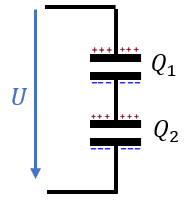
\includegraphics[scale=0.5]{img/kond1.png}} $\displaystyle \doubleunderline{Q_1 = Q_2 = Q}$
												\end{center}
											\iend

											\textbf{Begründung} \\
												Damit sich auf dem ersten Kondensator die Ladung $Q_1$ ansammeln kann, muss diese Ladung unterhalb des Kondensators angesammelt werden. Angenommen, beide Kondensatoren waren zu Beginn ungeladen,
												so muss die Ladung, welche sich auf der unteren Platte des ersten Kondensators befindet, dieselbe Ladungsmenge auf der oberen Platte des unteren Kondensators hervorrufen. \\

												\definition{Maschenregel bei Parallelschaltung}
												\beginip
													Die Maschenregel für Spannung gilt auch bei Kondensatoren
													\begin{center}
														\fix
															\ibox{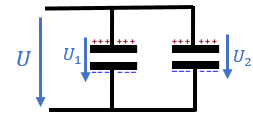
\includegraphics[scale=0.5]{img/kond2.png}}
															$\displaystyle \doubleunderline{U_1 = U_2 = U} $  und  $\displaystyle C_1 = \frac{Q_1}{U_1} \rightarrow \doubleunderline{Q_1 = C_1 \cdot U}$
													\end{center}
												\iend

												\definition{Grundlegende Gleichung am Kondensator}

												\beginip
												Der Zusammenhang zwischen Strom und Spannung am Kondensator ist wie folgt gegeben
												\formulaBegin
												$\displaystyle u_c(t) = \frac{1}{C} \int_0^t i_c(t) dt$ \\

												$\displaystyle i_c(t) = c \cdot \frac{d}{d t} (u_c)$ \\
												\formulaEnd
												\iend


												\textbf{Begründung} \\
													Mit dem Wissen, dass Strom definiert ist als die Ladung pro Zeit $ \displaystyle \frac{dQ}{dt} = I$ folgt folgendes: \\
													\begin{center}
													$\displaystyle \frac{\partial}{\partial t} (C \cdot U) = \frac{\partial}{\partial t} (Q) $ \\
													$ \displaystyle C  \cdot \frac{dU}{dt} = I \rightarrow U(t) = \frac{1}{C} \cdot \int_0^t I \cdot dt$
												\end{center}


\subsection{Strom}
\label{chap:Style}
Legen wir ein elektrisches Feld an einem Material mit beweglichen Ladungsträgern an,
so beginnen sich die Ladungsträger entlang dem angelegten Feld zu bewegen. \\
Je mehr freie Ladungsträger pro Volumen vorhanden sind ($:= \rho$), desto mehr Ladungsträger werden sich zu bewegen beginnen. \\
Die Geschwindigkeit ($:= v,$ Driftgeschwindigkeit), mit der sich die Ladungsträger bewegen, ist abhängig von der Stärke des elektrischen Feldes und
dem Material selbst. Wie gut sich ein Ladungsträger in einem Material bewegen kann, beschreiben wir mit der Beweglichkeit ($:= \mu$)


\important{Definition} {Strom und Stromdichte}
\beginip
Der Strom I bezeichnet, wie viele Teilchen sich pro Zeit durch eine Fläche bewegen. \\
Die Stromdichte J sagt etwas darüber aus, wie viel Strom pro Fläche fliesst \textbf{(= Dichte)}
\formulaBegin
$\displaystyle I := \frac{dQ}{dt} = \iint_A \vec{J} \cdot d\vec{A}$
\formulaEnd
\textbf{Variabeln}: \\
$ I = $ Strom $ [I] = A = \frac{C}{s}$ \\

\formulaBegin
$\displaystyle \vec{J} = \underbrace{n\cdot q}_{\rho} \vec{v} = \kappa \cdot \vec{E}$
\formulaEnd

\textbf{Variabeln}: \\
$ \vec{J} = $ Stromdichte $ [J] = \frac{A}{m^2}$ \\
$ n =$ Teilchendichte $ [n] = \frac{1}{m^3}$ \\
$ q =$ Ladungen der Teilchen$ [q] = C = As$ \\
$ \vec{v} = $ Driftgeschwindigkeit $ [v] = \frac{m}{s}$ \\
$ \rho = $ Raumladungsdichte $ [\rho] = \frac{As}{m^3}$ \\
$ \kappa = $ Elektrische Leitfähigkeit $ [\kappa] = \frac{A}{V\cdot m}$
\iend

Grundlage für den Strom sind bewegte Ladungsträger. \\
Im Falle eines Kupferkabel sind dies zum Beispiel Elektronen, die sich \textbf{gegen} das
elektrische Feld bewegen. Da Elektronen jedoch eine negative Ladung besitzen und der Strom als Ladung pro Zeit die durch eine Fläche hindurchfliesst definiert ist, zählen negative Ladungen, die entgegen dem Strom fliessen, zum Strom hinzu.

\begin{center}
	$\displaystyle J := n \cdot q \cdot \vec{v_I} = n \cdot (-e) \cdot (-\vec{v_I}) $
\end{center}

In anderen Baustoffen (wie zum Beispiel Halbleitern), bewegen sich \textbf{positive Ladungsträger} (=Löcher) mit dem Elektrischen Feld. \\
Diese führen zu einem positiven Strom in dessen Bewegungsrichtung. \\
Je nach Material, ist es auch möglich, dass beide Ladungsträger zum Stromfluss beitragen, sich jedoch nicht gleich gut im Material bewegen können. \\
Aus diesem Grund, gibt es für positive wie negative Ladungen verschiedene Beweglichkeiten.

\definition{Elektrische Leitfähigkeit}
\beginip
Die elektrische Leitfähigkeit ($\kappa$) beschreibt, wie gross die Stromdichte in einem Material, bei einem gegebenen E-Feld wird. \\
\formulaBegin
$\displaystyle \vec{J} = \kappa \cdot \vec{E} = \vec{J_{-}} + \vec{J_{+}} = \underbrace{(n_{-} \cdot q_{-} \cdot \mu_- + n_+ \cdot q_+ \cdot \mu_{+})}_{\kappa} \cdot \vec{E}$
\formulaEnd
Dabei bezeichnen die Variabeln $\mu_{x}$ die \textbf{Beweglichkeit} der einzelnen Ladungsträger und sind ein Mass dafür, wie schnell sich die Teilchen bei einem gegebenem E-Feld bewegen werden.
\iend


\subsection{Verhalten des J- und E-Feldes an Materialübergängen}
Triftt eine Stromdichte auf einen Materialübergang, so ändert sich der Betrag der Tangentialkomponente. Die \textbf{Normalkomponente bleibt gleich}.
\begingl
Es gilt bei Materialübergängen: \\
Für das J-Feld:
\fspace
\formulaBegin

$\displaystyle \frac{tan(\alpha_1)}{tan(\alpha_2)} = \frac{J_{t1}}{J_{t2}}  $ \\
\fspace
$\displaystyle J_{n1} = J_{n2}$

\formulaEnd

Für das E-Feld:
\fspace
\formulaBegin

$\displaystyle E_{t1} = E_{t2}$
$\displaystyle \frac{tan(\alpha_1)}{tan(\alpha_2)} = \frac{E_{n2}}{E_{n1}}  $ \\
\fspace

\formulaEnd
\iend

\newpage
%----------------------------------------------------------------
%
%  File    :  thesis-style.tex
%
%  Author  :  Keith Andrews, IICM, TU Graz, Austria
%
%  Created :  27 May 93
%
%  Changed :  19 Feb 2004
%
% styling and technical implementation adopted 2011 by Karl Voit
%----------------------------------------------------------------

					\section{Netzwerke}
					\label{chap:Style}


					\definition{Widerstand und Leitwert}

					\beginip
					Der \textbf{Widerstand} bestimmt, wieviel Strom fließen kann, wenn eine bestimmte Spannung angelegt wird. \\
					\begin{center}
						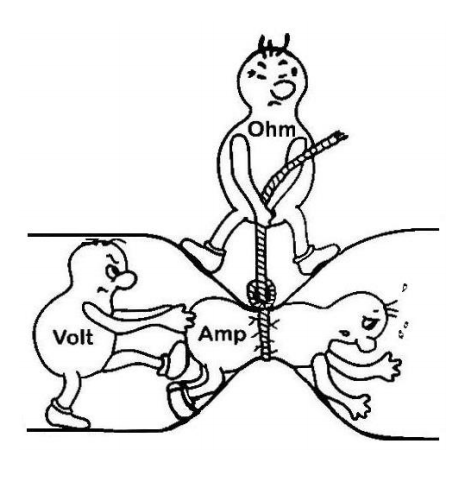
\includegraphics[scale=0.25]{img/widerstand.png}
					\end{center}
					\formulaBegin
					$ R :=  \frac{U}{I} =  \rho  \frac{l}{A},   {[R]} = \Omega, Ohm $
					\formulaEnd
					Als \textbf{Leitwert} bezeichnen wir die Inverse des Widerstandes. Er gibt an, wie groß die Spannung ist, wenn ein gewisser Strom fließt. \\
					\formulaBegin
					$ Y = \frac{1}{R} = \frac{A}{\rho \cdot l} $
					\formulaEnd
					\iend




										Da das elektrische Feld wirbelfrei ist, erhalten wir unabhängig vom Weg den gleichen Wert für die Spannung $ U_{AB} $ \\
										Dies bedeutet jedoch auch, dass wir für einen geschlossenen Weg die Spannung $0V$ erhalten müssen, da für jede geschlossene Kurve $\gamma$ gilt:
										\begin{center}
											\vspace{-2mm}

											$\displaystyle \oint_{\gamma} \vec{E} \cdot d\vec{s} = \int_{\gamma_0}^{\gamma_1} \vec{E} \cdot d\vec{s} + \int_{\gamma_1}^{\gamma_0} \vec{E} \cdot d\vec{s} = U_{01} + U_{10} = 0$
										\end{center}
										Mit dieser Erkenntnis können wir die Maschenregel definieren:

										\definition{Maschenregel}
										\beginip
										Die Summe aller Spannungen in einer Masche ergibt $0$ \\
										\formulaBegin
										$\displaystyle \sum_{k=1}^n U_k = 0$
										\formulaEnd

										\iend

										\begin{minipage}{0.6\textwidth}
											\begin{flushright}
											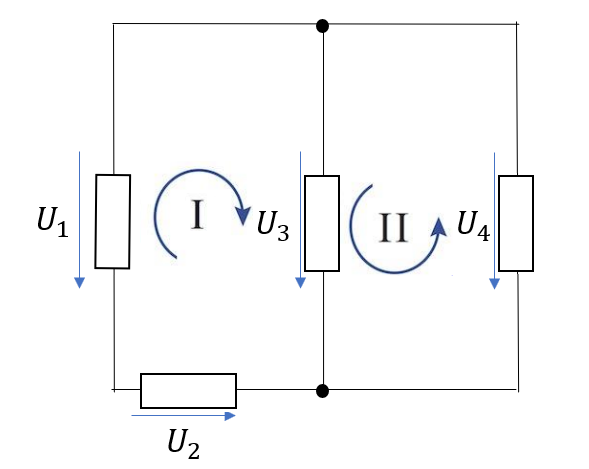
\includegraphics[scale=0.45]{img/maschenregel-2.png}
										\end{flushright}
										\end{minipage}
										\begin{minipage}{0.4\textwidth}
											\textbf{Maschenregel} \\ \\
											I: $\displaystyle (- U_1) + U_3 + (-U_2)  = 0$ \\
											II: $\displaystyle U_3 + (- U_4) = 0 $ \\
											% \vspace{1.5cm}
										\end{minipage}

										Analog können wir mithilfe der Ladungserhaltung argumentieren, dass sämtliche Ladungen, welche in ein Gebiet hineinfließen, auch wieder aus diesem hinausließen müssen.

										\definition{Knotenregel}
										\beginip
										Die Summe aller Ströme die in einen Knoten hinein/hinausfließen muss $0$ ergeben. \\
										\formulaBegin
										$\displaystyle\sum_{i=0}^n I_n = 0 $
										\formulaEnd
					          \iend

										\textbf{Wichtig} Die Knotenregel kann auch auf ein Gebiet von Knoten angewandt werden. \\


										\begin{minipage}{0.6\textwidth}
										\begin{flushright}
												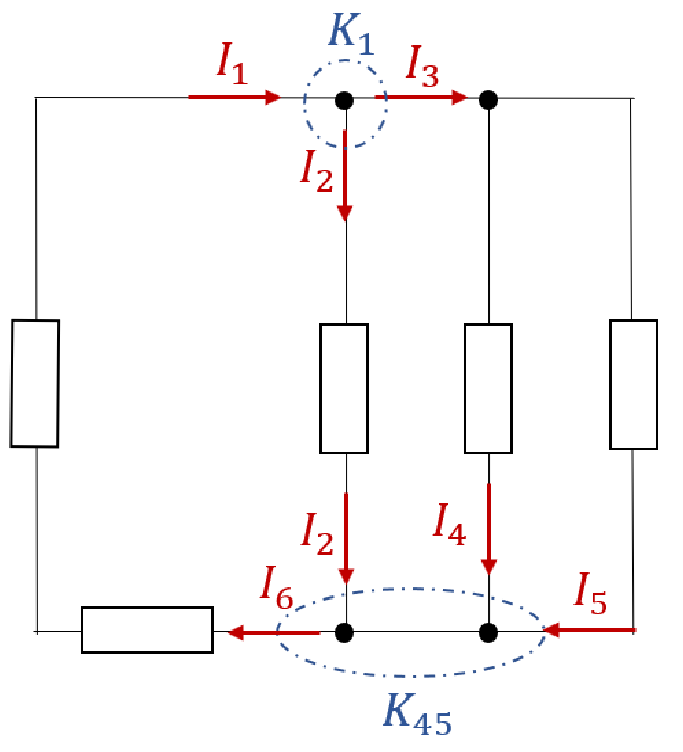
\includegraphics[scale=0.4]{img/knotengl.png}
											\end{flushright}
										\end{minipage}
										\begin{minipage}{0.4\textwidth}

											\textbf{Knotengleichungen} \\ \\
											$\displaystyle K_1$: $ I_1 - I_2 - I_3 = 0 $ \\
											$\displaystyle K_{45}$: $ I_2 + I_4 + I_5 - I_6 = 0 $ \\
										\end{minipage}


					\newpage

										\subsection{Grundlegende Netzwerkumformungen}
										Wir interessieren uns nun dafür, wie sich Widerstände verhalten, wenn wir sie seriell/parallel verknüpfen.
										\definition{Serienschaltung}
										\beginip
										Werden mehrere Widerstände seriell miteinander verbunden, so addieren sich die Widerstandswerte \\
										\formulaBegin
										$\displaystyle R_{serie} = \sum_{i=0}^n R_i $
										\formulaEnd
										\iend

							        \vspace{1em}

										\textbf{Begründung} \\
										Mehrere Widerstände in Serie können als ein langer Widerstand mit konstanter Fläche angesehen werden. Da die Längenabhängigkeit des Widerstandes im Zähler steht, addieren sich die Werte. \\
										$\displaystyle R_s = \rho \cdot \frac{l_1+l_2}{A} = \rho \cdot \frac{l_1}{A}  + \rho \cdot \frac{l_2}{A}  = R_1 + R_2 $
										\fix
										\begin{center}
											\ibox{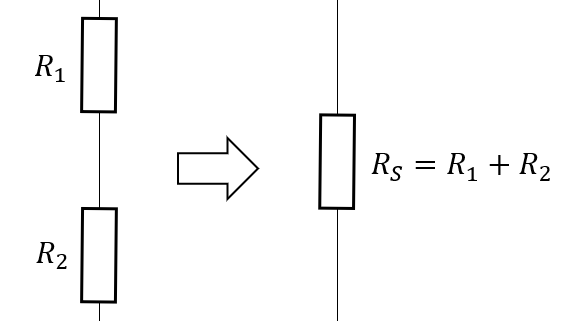
\includegraphics[scale=0.3]{img/serienschaltung.png}}
										\end{center}
					\fix


										\definition{Parallelschaltung}

										\beginip
										Werden mehrere Widerstände parallel miteinander verbunden, so addieren sich die Leitwerte \\
										\formulaBegin
										$\displaystyle Y_{parallel} = \sum_{i=0}^n Y_i \Bigg\rvert$
										$\displaystyle R_{parallel} = \left(\sum_{i=0}^n \frac{1}{R_i}\right)^{-1}$
										\formulaEnd
										\iend

					          \vspace{1em}

					          \textbf{Begründung} \\
										Mehrere Widerstände parallel können als ein Widerstand mit größerer Fläche und konstanter Länge angesehen werden. Da die Flächenabhängigkeit des Widerstandes im Nenner steht, addieren sich die Leitwerte. \\
											$\displaystyle Y_p = \frac{1}{\rho} \cdot \frac{A_1 + A_2}{l} = \frac{1}{\rho} \cdot \frac{A_1}{l}  + \frac{1}{\rho} \cdot \frac{A_2}{l}  = Y_1 + Y_2 $


										\begin{center}
											\ibox{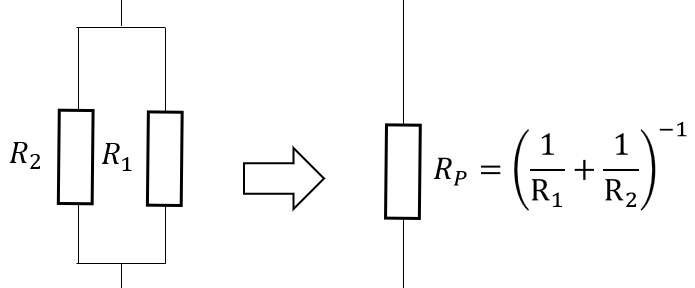
\includegraphics[scale=0.3]{img/parallel.png}}
										\end{center}




										\subsection{Stern Dreieck Umformung}
										\begin{center}
											%todo fix
		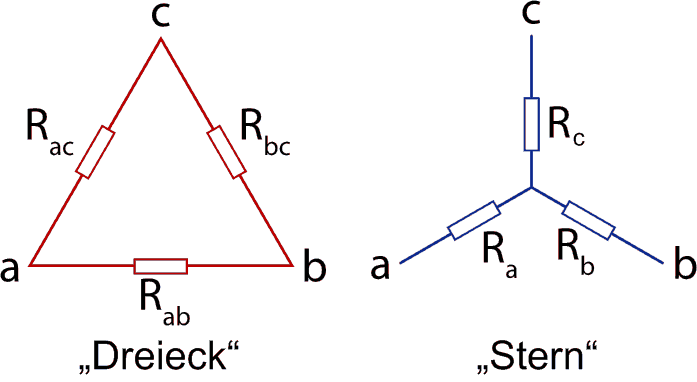
\includegraphics[scale=0.3]{img/Stern-Dreieck-Transformation.png}
\end{center}
	\begin{multicols*}{2}
		$\underline{R}_{AB}=\frac{\underline{R}_{A}\underline{R}_{B}+\underline{R}_{B}\underline{R}_{C}+\underline{R}_{A}\underline{R}_{C}}{\underline{R}_{C}}$\\
		$\underline{R}_{AC}=\frac{\underline{R}_{A}\underline{R}_{B}+\underline{R}_{B}\underline{R}_{C}+\underline{R}_{A}\underline{R}_{C}}{\underline{R}_{B}}$\\
		$\underline{R}_{BC}=\frac{\underline{R}_{A}\underline{R}_{B}+\underline{R}_{B}\underline{R}_{C}+\underline{R}_{A}\underline{R}_{C}}{\underline{R}_{A}}$\\
		$\underline{R}_A=\frac{\underline{R}_{AC}\underline{R}_{AB}}{\underline{R}_{AC}+\underline{R}_{AB}+\underline{R}_{BC}}$\\
		$\underline{R}_B=\frac{\underline{R}_{AB}\underline{R}_{BC}}{\underline{R}_{AC}+\underline{R}_{AB}+\underline{R}_{BC}}$\\
		$\underline{R}_C=\frac{\underline{R}_{AC}\underline{R}_{BC}}{\underline{R}_{AC}+\underline{R}_{AB}+\underline{R}_{BC}}$
	\end{multicols*}




										\definition{Spannungsteiler}
										\beginip
										Die Spannungsteilerregel gibt an, wie sich eine Spannung über verschiedene Widerstände aufteilt, wenn diese in \textbf{Serie} geschaltet sind. \\
											\formulaBegin
											$\displaystyle U_{R_x} = U_{ges} \cdot \frac{R_X}{\sum R_i} $
											\formulaEnd

											\begin{center}
												\ibox{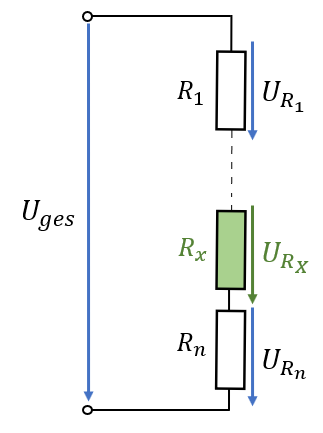
\includegraphics[scale=0.4]{img/spannungsteiler.png}}
											\end{center}
										\iend


										\textbf{Begründung} \\
											Gemäss $\displaystyle U = R \cdot I $ und der Serienschaltung ist der Strom durch alle Widerstände gegeben als $\displaystyle I = \frac{U_{ges}}{\sum R_i} $ \\
											Nun müssen wir nur noch den Strom mit dem gesuchten Widerstand multiplizieren um die Spannung zu erhalten: $\displaystyle U_{R_X} = R_X \cdot I = R_X \frac{U_{ges}}{\sum R_i} $

					\fix
										\definition{Stromteiler}
										\beginip
											Die Stromteilerregel gibt uns an, wie sich die Ströme in einem Knoten aufteilen, wenn die Widerstände \textbf{parallel} geschaltet sind.
											\fspace
											\formulaBegin
											$\displaystyle I_x = I_{in} \cdot \frac{(R_1 || ... || R_n)} {R_x} $
											\formulaEnd
					\fix
											\begin{center}
												\ibox{\includegraphics[scale=0.3]{img/stromteiler.png}}
											\end{center}
											\fix
											\textbf{Spezialfall} 2 Widerstände \\
											Falls der Stromteiler nur mit zwei Widerständen angewendet wird, vereinfacht sich die Formel:
											\fspace
											\formulaBegin
											$\displaystyle I_x = I_{in} \cdot \frac{R_y}{R_x + R_y} $
											\formulaEnd
											Der Widerstand, dessen Strom uns \textbf{nicht} interessiert, steht hierbei im Zähler!
										\iend

										\subsubsection{Grundregeln bei Netzwerkumformungen}
					\fix \fix
										\important{Regel 1}{Expandieren von Knoten}
										\beginip
										 	Knoten können aufgeteilt und mit Verbindungslinien verbunden werden\\
											\begin{center}
											\ibox{\includegraphics[scale=0.25]{img/knotenexp.png}}
											\end{center}
										\iend

										\fix
					\fix \fix
										\important{Regel 2}{Verschieben von Elementen}
										\beginip
											Elemente können entlang von \textbf{Verbindungslinien ohne Widerständen} verschoben werden\\
											\begin{center}
												\fix \fix \fix
											\ibox{\includegraphics[scale=0.3]{img/verschieben.png}}
											\end{center}
										\iend
					\fix \fix
										\important{Regel 3}{Vertauschen von Elementen in Serie}
										\beginip
											Elemente, die \textbf{in Serie} geschaltet sind, können vertauscht werden
											\begin{center}
												\fix
											\ibox{\includegraphics[scale=0.3]{img/vertausch-serie.png}}
											\end{center}
										\iend
					\fix \fix
										\important{Regel 4}{Vertauschen von parallel geschalteten Elementen}
										\beginip
											Elemente die \textbf{parallel} geschaltet sind, können vertauscht werden
											\begin{center}
												\fix
											\ibox{\includegraphics[scale=0.3]{img/vertausch-parallel.png}}
											\end{center}
										\iend
					\fix \fix
										\important{Regel 5}{Knoten kontrahieren}
										\beginip
											(Analog zu 1) Knoten können zusammengezogen werden, sofern sie nicht durch einen Widerstand verbunden sind.
											\begin{center}

											\ibox{\includegraphics[scale=0.3]{img/knoten-kontrahieren.png}}
											\end{center}
										\iend

										\newpage


										\subsection{Vereinfachungen mithilfe Symmetrieüberlegungen}

										Besitzt ein Netzwerk verschiedene Punkte mit dem selben Potential, so können diese Punkte beliebig verbunden werden.
										Da die Potentialdifferenz immer 0 sein wird, wird niemals Strom zwischen diesen Punkten fliessen.

										\bsptask{Beispiel}{Vereinfachung eines Netzwerkes mit Symmetrie}
										\beginbsp
											Fassen sie alle Widerstände zu einem zusammen unter verwendung der Symmetrieeigenschaften
											\begin{center}
												\ibox{ \includegraphics[scale=1.3]{img/sym.png}}
											\end{center}
										\iend

										\bsp{Lösung}{}
										\beginbsp
										Da das Widerstandsnetzwerk symmetrisch bezüglich $R_2$ ist, muss am Punkt 2 und am Punkt 4 das gleiche Potential existieren. \\
										Dies bedeutet, dass über dem Widerstand $R_2$ niemals eine Spannug abfallen und somit auch nie Strom fliessen wird. \\
										\textbf{Lösung 1}: \\
										Wir verbinden die Punkte 2 und 4 mit einem Kurzschluss und erhalten
										\begin{center}
											\ibox{ \includegraphics[scale=1]{img/sym-l1.png}}
											$\doubleunderline{R_{ges}} = (R_1 || R_1) + (R_3 || R_3) = \doubleunderline{\frac{1}{2}(R_1 + R_3)}$
										\end{center}

										\textbf{Lösung 2}: \\
										Wir verbinden die Punkte 2 und 4 mit einem Leerlauf und erhalte
										\begin{center}
												\ibox{ \includegraphics[scale=1]{img/sym-l2.png}}
											$\doubleunderline{R_{ges}} = \big( (R_1 + R_3) || (R_1 + R_3) \big) = \doubleunderline{\frac{1}{2}(R_1 + R_3)}$
										\end{center}


										\iend




										\subsection{Vorgehen um Schaltbilder mit einer Quelle zu vereinfachen}
										\begin{enumerate}
											\item Bringe Quelle auf die linke Seite
											\item Forme mit Regel 1 - 5 das Netzwerk soweit um, bis nur noch Spannungs-/Stromteiler oder einfache Maschen vorhanden sind.
											\item Expandiere nun das Netzwerk Schritt für Schritt, bis die Spannung über dem gesuchten Widerstand berechnet werden kann.
										\end{enumerate}

										\bsptask{Beispiel}{\#1}
										\beginbsp
										1) Berechnen sie $U_x$ in Abhängigkeit des Quellstromes $I$
										\begin{center}
											\fix
										 \ibox{\includegraphics[scale=0.55]{img/aufg1-aufg.png}}
										\end{center}
										\fix
										 \textbf{Lösung}
									 \begin{enumerate}
					  				 \item Gemäss Regel 2 können wir $R_1$ und die Stromquelle vertauschen.
										 \item Die Widerstände $R_4 , R_5$ und $ R_x $ können zu $ R_S = R_3 + R_4 + R_5 $ zusammengefasst werden.
										 \item Mithilfe der Stromteilerregel erhalten wir $ I_s = I \cdot \frac{(R_1 || R_2 || R_s)}{R_s} $ und somit $U_s = I \cdot (R_1 || R_2 || R_S) $
										 \item Die Spannung $U_s$ liegt also über dem Widerstand $R_s$ an. Wenn wir diesen wieder in die ursprünglichen 3 Widerstände aufteilen, erhalten wir mithilfe der Spannungsteilerregel $U_x = U_s \cdot \frac{R_x}{R_4 + R_5 + R_x} $
									 \end{enumerate}

										\ibox{\includegraphics[scale=0.55]{img/bsp1.png}}
										\iend

										In manchen Fällen kann es schwierig sein, die Quelle auf die linke Seite zu bringen oder das Schaltbild nützlich umzuformen. \\
										Um ein erstes Ersatzschaltbild zu erhalten, kann das "Flussverfahren\texttt{"} angewandt werden.

					\newpage
										\bsp{Beispiel}{Flussverfahren}
										\beginbsp
										Beim Flussverfahren überlegt man sich sämtliche Arten, wie der Strom von einem Ende der Quelle zum anderen fliessen kann, und zeichnet somit ein Ersatzschaltbild. \\ \\
										\textbf{Beispiel}
										\begin{center}
											\fix
												\ibox{\includegraphics[scale=0.3]{img/fluesse.png}}
										\end{center}
										\iend

										\subsection{Quellen}
										\definition{Ideale Quelle}
										\beginip
										Eine ideale Strom-/Spannungsquelle liefert immer denselben Strom/dieselbe Spannung, unabhängig von der Last, welche angehängt wird.
										\begin{center}
											\ibox{\includegraphics[scale=0.6]{img/ideale_quelle.png}}
										\end{center}

										\iend


										Mit idealen Strom-/Spannungsquellen können wir theoretisch unendlich viel Spannung/Strom über einem Lastwiderstand erzeugen. \\
										(Beispiel ideale Spannungsquelle im Kurzschluss/ideale Stromquelle im Leerlauf) \\
										Bei einer realen Quelle kann jedoch nur eine endliche Spannung/Strom auftreten, wesshalb wir Verluste innerhalb der Quelle mit einem Innenwiderstand $R_i$ modellieren. \\

										\definition{Reale Quelle}
										\beginip
										Eine reale Quelle bezeichnet eine ideale Quelle mit Vorwiderstand. \\
										Bei einer \textbf{Stromquelle} ist der Widerstand \textbf{parallel}, bei einer \textbf{Spannungsquelle} ist der Widerstand in \textbf{Serie}.
											\begin{center}
												\fix
													\ibox{\includegraphics[scale=0.7]{img/realeQuellen.png}}
											\end{center}
										\iend




																				\subsection{Superpositionsprinzip}

																				 Das Superpositionsprinzip besagt, dass wir bei einem Netzwerk mit mehreren Quellen einzelne Teillösungen in Abhängigkeit von nur einer Quelle berechnen und aufsummieren können. \\
																				 Dies gilt jedoch nicht für die Leistung, da diese nicht linear ist! \\
																				 Um das Superpositionsprinzip anzuwenden, müssen wir alle ausser eine Quelle auf \texttt{"}0\texttt{"} setzen. \\
																				 Spannungsquellen werden also mit \textbf{Kurzschlüssen} ersetzt und Stromquellen mit \textbf{Leerläufen}. \\
																				 \begin{center}
																				 	\fix
																				 		\ibox{\includegraphics[scale=0.3]{img/superpos-zero.png}}
																				 \end{center}


																				 \textbf{Wieso} \\
																				 Eine Spannungsquelle zu \texttt{"}0\texttt{"} zu setzen bedeutet, dass über diesem Bauteil keine Spannung abfallen darf. Über einem Kurzschluss wird nie eine Spannung abfallen, da dieser als Widerstand mit Wert 0 modelliert werden kann. \\
																				 Eine Stromquelle zu \texttt{"}0\texttt{"} zu setzen bedeutet, dass durch dieses Bauteil kein Strom fliessen darf. Dies entspricht gerade einem Leerlauf, da dieser als Widerstand mit Wert $\displaystyle \rightarrow \infty$ modelliert werden kann. \\


																				 \bsptask{Beispiel}{\#2}
																				 \beginbsp
																					\textbf{Aufgabe} Berechnen sie die Spannung $U_x$ und die Leistung $P_x$ im folgenden Netzwerk, wenn alle Widerstände $ R = 100 \Omega$ betragen. \\
																					\begin{center}
																						\fix
																					\ibox{\includegraphics[scale=0.6 ]{img/ex2-1.png}}
																					\end{center}
																					\iend

																					\beginip
																					\textbf{Lösung}
																					\\
																					Zuerst setzen wir die Spannungsquelle zu 0 und erhalten das folgende ESB \\
																					\begin{center}
																						\fix
																					\ibox{\includegraphics[scale=0.5 ]{img/ex2-2.png}}
																					\end{center}

																					Nun berechnen wir den Strom $I_{x_1}$ durch den Widerstand mithilfe eines Stromteilers: \\
																					$I_{x_1} = 60mA$ \\
																					Die Spannung $U_x$ ist entgegen der Stromrichtung eingezeichnet: \\
																					$U_{x_1} = - R_x \cdot I_x = - 100 \cdot 60mA = -6V $ \\
																					\\
																					Nun setzen wir die Stromquelle zu 0: \\
																					\begin{center}
																						\fix
																					\ibox{\includegraphics[scale=0.5 ]{img/ex2-3.png}}
																					\end{center}

																					Die Spannung $U_{x_2}$ berechnet sich als Spannungsteiler: \\
																					$U_{x_2} = 20V \cdot \frac{100\Omega}{400\Omega} = 5V$ , $ I_{x_2} = \frac{5V}{100\Omega} = 50mA $\\
																					\\
																					Schlussendlich berechnet sich die Spannung als Summe der Teilspannungen:
																					$U_x = U_{x_1} + U_{x_2} = 5V -6V = -1V $ \\
																					Und die Leistung: \\
																					$P_x = \frac{{U_x}^2}{R_x} = 10mW$ \\
																					Welche \textbf{nicht} der Summe der Teilleistungen entspricht: \\
																					$P_{sum} = P_1 + P_2 = U_{x_1} \cdot I_{x_1} + U_{x_2} \cdot I_{x_2} = 360mW + 250mW = 610mW$


																				 \iend



																				\subsection{Ersatzquelllen}


																				\definition{Thévenin / Norton Äquivalent}
																				\beginip
																				Jedes Netzwerk mit \textbf{linearen} Bauelementen und 2 Klemmen lässt sich als reale Quelle darstellen. \\
																				\textbf{Thévenin Äquivalent} Darstellung als reale \textbf{Spannungsquelle} mit Leerlaufspannung, die an den Klemmen auftritt \\
																				\textbf{Norton Äquivalent} Darstellung als reale \textbf{Stromquelle}  mit Kurzschlussstrom, der an den Klemmen auftritt\\
																				Der Innenwiderstand entspricht dem von außen gemessenen Widerstand, wenn alle Quellen zu 0 gesetzt werden.
																				\begin{center}
																					\fix
																						\ibox{\includegraphics[scale=0.6]{img/nort_the.png}}
																				\end{center}
																				\iend


																				\newpage
																				\vorgehen{Vorgehen}{Ersatzquelle für gegebenes Schaltbild mit offenen Klemmen finden}
																				\beginvor
																				\begin{itemize}

																				  \item[1.] Betrachte die Schaltung. Sind mehr Stromquellen vorhanden, so ist es häufig einfacher den Kurzschlussstrom zu berechnen. Bei mehr Spannungsquellen die Leerlaufsspannung. \\
																				  Wiederhole folgendes für alle Quellen $i$: \\
																				  \end{itemize}
																				  \beginip
																				  \begin{itemize}

																				  \item [2.  ]  Setze alle Strom / Spannungsquellen ausser einer zu 0. (Stromquelle $\rightarrow$ Leerlauf, Spannungsquelle $\rightarrow$ Kurzschluss)
																				  \item[3. ] Versuche die einzelne Quelle auf die linke Seite zu bekommen. (Siehe Skript \texttt{"}Flussverfahren\texttt{"})
																				  \item[4.a)] \textbf{Kurzschlussstrom}
																				  \begin{enumerate}
																				  \item Schliesse die Klemmen kurz und bezeichne den Strom, welcher durch diese Klemmen fliesst als $I_{ks}^{(i)}$.
																				  \item Versuche mittels Stromteilern den gesuchten Strom zu berechnen. Falls eine direkte Verbindung von Stromquelle über den Kurzschluss zur Quelle zurückfürt, ist der Kurzschlussstrom gleich dem Strom der Quelle (=0 bei Spannungsquelle). \\
																				  Ist die Quelle keine Stromquelle, so kann evt. ein serieller Widerstand verwendet werden, um die Quelle umzuformen.
																				  \end{enumerate}
																				  \item[4.b)] \textbf{Leerlaufspannung}
																				  \begin{enumerate}
																				  \item Zeichnen einen Spannungspfeil zwischen den Klemmen und bezeichne die Spannung als $U_{LL}^{(i)}$.
																				  \item Versuche mittels Spannungsteiler die gesuchte Spannung zu berechnen. Falls kein Strom von der Spannungsquelle fliessen kann (Leerlauf unterbricht die komplette Schaltung), so ist die Leerlaufspannung gleich der Spannung der Spannungsquelle (=0 bei Stromquelle). \\
																				  Ist die Quelle keine Spannungsquelle, so kann evt. ein paralleler Widerstand verwendet werden, um die Quelle umzuformen.
																				  \end{enumerate}
																				\end{itemize}

																				  \iend
																				\begin{itemize}

																				  \item[5] \textbf{Innenwiderstand}
																				  \begin{enumerate}
																				    \item Setze \textbf{alle} Quellen auf 0. Versuche nun die Widerstände solange umzuformen, bis nur noch ein Ersatzwiderstand vorhanden ist. (Ggf. \texttt{"}Flussverfahren\texttt{"} mit offener Klemme anwenden)
																				    \item Bezeichne den Wert des Widerstandes als $R_i$
																				  \end{enumerate}
																				  \item[6.a)] \textbf{Thévenin Äquivalent} Spannungsquelle mit seriellem Innenwiderstand. \\
																				  Werte: $\displaystyle   R= R_i$, $U_q = \sum_i U_{LL}^{(i)} = (\sum_i I_{ks}^{(i)})\cdot R_i$

																				  \item[6.b)] \textbf{Norton Äquivalent} Spannungsquelle mit parallelem Innenwiderstand. \\
																				  Werte: $\displaystyle  R= R_i$, $I_q = \sum_i I_{ks}^{(i)}) = \frac{\sum_i U_{LL}^{(i)}}{R_i}$

																				  \end{itemize}

																				\iend






																				\bsptask{Beispiel}{\#3 - Thévenin Äquivalente Schaltung}
																				\beginip
																				\textbf{Aufgabe}
																				\\Geben sie eine Thévenin Äquivalente Schaltung (Innenwiderstand $R_i$, $U_{Th}$) für folgende Klemmen an. Alle Widerstände haben Wert $100\Omega$ \\

																				\begin{center}
																					\fix
																						\ibox{\includegraphics[scale=0.4]{img/ex3-1.png}}
																				\end{center}
																				\iend
																				\beginip
																				\textbf{Lösung}
																				\\
																				Zuerst berechnen wir die Leerlaufspannung für die Stromquelle: \\
																				$U_{LL_1} = 120mA \cdot 200 \Omega = 24V$ \\
																				Danach die Leerlaufspannung für die Spannungsquelle: \\
																				$ U_{LL_2} = 20V$\\
																				Die Gesamtspannung und somit die Spannung der Ersatzspannungsquelle beträgt: \\
																				$\doubleunderline{U_{Th}} = U_{LL_1} + U_{LL_2} = \doubleunderline{44V}$ \\

																				Nun müssen wir noch den Innenwiderstand berechnen. Dazu setzen wir alle Quellen zu 0 und berechnen den von aussen gemessenen Widerstand:\\
																				\begin{center}
																					\fix
																						\ibox{\includegraphics[scale=0.6]{img/ex3-2.png}}
																				\end{center}
																									$\doubleunderline{R_i} = 100\Omega + 100\Omega  + 100\Omega  = \doubleunderline{300 \Omega} $
																				\iend


										\subsection{Leistungsanpassung}
										\definition{Leistung}
										\beginip
											Als Leistung bezeichnen wir das Produkt von Strom und Spannung. \\
											Sie bezeichnet die in einer Zeitspanne umgesetzte Energie an einem Bauteil. \\
											\formulaBegin
											$\displaystyle P := U \cdot I = \frac{U^2}{R} = I^2 \cdot R $
											\formulaEnd
										\iend

										\definition{Maximale Leistung}
										\beginip
										Um bei einer realen Quelle maximale Leistung an einen Lastwiderstand abzugeben, muss der Lastwiderstand gleich gross sein wie der Innenwiderstand der Quelle. \\
										\formulaBegin
										$ R_i = R_L \Rightarrow P = P_{max}$
										\formulaEnd
										\begin{center}
											\ibox{\includegraphics[scale=0.5]{img/leistungsanpassung.png}}
										\end{center}
										\iend

					\newpage
										\textbf{Begründung} \\
										Die Leistung an einem Lastwiderstand in Serie ist gegeben als: \\
										$ \displaystyle P_L = U_L \cdot I_L = \frac{U_L^2}{R_L} = \frac{( U_0 \frac{R_L}{R_L + R_i})^2}{R_L} = U_o^2 \cdot \frac{R_L}{(R_L + R_i)^2}$ \\
										$\displaystyle \frac{d}{dR_L} (P_L) = - U_0^2 \cdot \frac{R_L - R_i}{(R + R_L)^3} = 0 \Rightarrow R_L = R_i  \Rightarrow P_L = P_{max}$





















																														\newpage
																														\vorgehen{Vorgehen}{Leistung über einer Last Maximieren}
																														\beginvor
\textbf{Falls möglich}
\begin{itemize}
  \item [1. ] Entferne Komponenten über denen die Leistung maximiert werden soll und ersetze sie mit offenen Klemmen (Fasse die entfernten Komponenten als einen Lastwiderstand zusammen).
  \item [2. ] Berechne von den Klemmen den Innenwiderstand.
  \item [3. ] Innenwiderstand $R_i \rightarrow R_L = R_i$
  \item [4. ] Falls maximale Leistung gefragt: Berechne Leerlaufspannung oder den Kurzschlussstrom. $\displaystyle P_{max} = \frac{U_{LL}^2} {4 \cdot R_i } $
\end{itemize}

\textbf{Sonst}

\begin{itemize}
  \item [1. ] Finde einen Ausdruck für $U_L$ und $I_L$
	\item [2. ] Berechne $P = U_L \cdot I_L$
	\item [3. ] Leite $P$ nach dem veränderlichem Widerstand ab und setze zu 0 um ein Maximum zu finden
\end{itemize}


																														\iend

\bsptask{Beispiel}{Leistungsanpassung}
\beginbsp
Berechnen sie für folgendes ESB den Wert für $R_L$ bei dem $R_L$ maximale Leistung aufnimmt.
\begin{center}
	\ibox{\includegraphics[scale=0.2]{img/leistungsanp.png}}
\end{center}
\iend

\bsp{Lösung}{}
\beginbsp
Um die Leistung über $R_L$ zu maximieren, entfernen wir den Widerstand und berechnen den Innenwiderstand bezüglich den Klemmen. \\
Für die Berechnung des Innenwiderstandes, werden alle Spannungsquellen kurzgeschlossen.
\begin{center}
	\ibox{\includegraphics[scale=0.6]{img/leistungsanp_lsg.png}}
\end{center}
Nun müssen nur noch alle Widerstände zu einem Zusammengefügt werden:
\begin{center}
	$R_i = (R_1 || R_2 + (R_3 || R_4 )) = 2 \Omega$ \\
	$\doubleunderline{ R_L = R_i = 2 \Omega}$
\end{center}
\iend










										 \newpage





					          \subsection{Analyse umfangreicher Netzwerke}

					           Möchten wir in Netzwerken sehr viele Grössen berechnen, oder ist das Netzwerk sehr komplex, so können andere (meist Computer basierende) Verfahren verwendet. \\
					           Sämtliche Verfahren bauen darauf auf, dass für ein beliebiges Netzwerk das Aufstellen sämtlicher Konten und Maschengleichungen genügt, um alle gesuchten Grössen zu berechnen. \\

					          \important{Unabhängige Gleichungen}{}
					          \beginip
					             Seien z die Anzahl Zweige eines Netzwerkes (Verbindungen 2-er Knoten) und k die Anzahl Knoten, so müssen z linear unabhängige Gleichungen gefunden werden, um alle Grössen im Netzwerk zu berechnen.  \\Die Gleichungen können folgendermassen gefunden werden: \\
					             \formulaBegin
					              (k-1) Gleichungen können aus Knotengleichungen gefunden werden. \\
					              (z - (k-1)) übrige Gleichungen werden mithilfe von Maschengleichungen gefunden.
					             \formulaEnd
					           \iend



					           \vorgehen{Vorgehen}{Analyse von Umfangreichen Netzwerke}{}
					           \beginip
					            \begin{center}
					              \begin{itemize}
					                \item Entferne alle Widerstände und Quellen und zeichne das Schaltbild neu.
					                \item Nummeriere alle Konten. Die Anzahl der Knoten wird mit k bezeichnet.
					                \item Alle Verbindungslinien, welche zwei Knoten verbinden, werden als Zweige bezeichnet. \#Zweige = z
					                \item Definiere Ströme für jeden Zweig und stelle (k-1) Knotengleichungen auf. Schreibe diese am Besten bereits in Matrix schreibweise: \\
					                Bsp: $I_1 + I_2 = I_3, I_3 - I_4 = 2A $: \\
					                $
					 \left[ {\begin{array}{cccc}
					    1 & 1 & -1 & 0 \\
					    0 & 0 & 1 & -1 \\					\end{array} } \right] \left[ {\begin{array}{c} I_1 & I_2 & I_3 & I_4 \\ \end{array} } \right] =   \left[ {\begin{array}{c}  0 & 2A\\ \end{array} } \right] $ \\

					                \item Finde z - (k-1) Unabhängige Maschengleichungen. (Mittels Vollständiger Baum / Auftrennen der Maschen)
					                \item Ersetze die Spannungen der Maschengleichung mit Strom mal Widerstand und ergänze das Gleichungssystem.
					                \\ Bsp:
					                $U_1 + U_2 = 5V, U_2 - U_3 = U_4$ \\ $ \rightarrow R_1 \cdot I_1 + R_2 \cdot I_2 = 5V, R_2 \cdot I_2 - R_3 \cdot I_3 - R_4 \cdot I_4 = 0$ \\
					                $
					 \left[ {\begin{array}{cccc}
					    1 & 1 & -1 & 0 \\
					    0 & 0 & 1 & -1 \\
					    \mathbf{R_1} & \mathbf{R_2} & 0 & 0 \\
					    0 & \mathbf{R_2} & \mathbf{-R_3} & \mathbf{-R_4} \\
					\end{array} } \right] \left[ {\begin{array}{c} I_1 & I_2 & I_3 & I_4 \\ \end{array} } \right] =   \left[ {\begin{array}{c}  0 & 2A & \mathbf{5V} & \mathbf{0} \\ \end{array} } \right] $ \\

					              \end{itemize}
					            \end{center}
					            \iend

%----------------------------------------------------------------
%
%  File    :  thesis-style.tex
%
%  Author  :  Keith Andrews, IICM, TU Graz, Austria
%
%  Created :  27 May 93
%
%  Changed :  19 Feb 2004
%
% styling and technical implementation adopted 2011 by Karl Voit
%----------------------------------------------------------------
\newpage
\section{Magnetostatik}
\subsection{Das Magnetische Feld und die Lorentzkraft}

	Analog zum elektrischen Feld definieren wir ein magnetisches Feld, dessen Feldlinien Kräfte auf eine bewegte Ladung auswirken. \\
	Auslöser für das magnetische Feld sind \textbf{bewegte Ladungen} welche gemäss der rechten Hand Regel ein Magnetfeld hervorrufen, das diese einschliesst. \\
\begin{center}

\ibox{\includegraphics[scale=0.3]{img/hfeld.png}}

	\end{center}
	\definition{Magnetische Flussdichte \textbf{B}}
	\beginip
	Bewegte Ladungsträger welche sich in der Nähe anderer bewegter Ladungsträger befinden, verspüren eine Kraftwirkung welche senkrecht zur Bewegungsrichtung zeigt. \\
	Analog zum Elektrischen Feld definieren wir ein Magnetisches Feld (= Magnetische Flussdichte) welche diese Kraftwirkung beschreibt. \\
	Die Mangetische Flussdichte, weisst jedem Punkt im Raum einen Vektor zu. Die Resultierende Kraft auf ein Ladungsträger, welcher sich mit Geschwindigkeit V bewegt,
	berechnet sich aus dem Kreuzprodukt von Geschwindigkeit und Ladung ($\rightarrow$ \textbf{Lorentzkraft})
	\iend




	\definition{Rechte Hand Regel}
	\beginip
	Die Magnetische Flussdichte $B$ um einen stromdurchflossenen Leiter baut sich stets gegen den Uhrzeigersinn auf und ist \textbf{immer} geschlossen. \\
	\begin{center}
			\ibox{\includegraphics[scale=0.2]{img/rechte-hand-regel.png}}
	\end{center}
	\iend

	\gl{Gleichung}{Lorentzkraft}
	\begingl
	Bewegte Ladungen in einem Magnetfeld verspüren eine Kraft, welche proportional zur Stärke des B-Feldes und der Geschwindigkeit ist. \\
	Die Kraft steht senkrecht zu den Feld- und Geschwindigkeits-Vektoren.


	\begin{center}
			\ibox{\includegraphics[scale=0.3]{img/lorentzkraft.png}}
	\end{center}

	\formulaBegin
	$\vec{F_m} = q \cdot \vec{v} \times \vec{B} = I(\vec{l} \times \vec{B})$
	\formulaEnd

	\textbf{Variabeln}: \\
	$ F_m = $ Magnetische Kraft $ [F_M] = N$ \\
	$ \vec{v} = $ Geschwindigkeit der Teilchen $ [v] = \frac{m}{s}$ \\
	$ \vec{B} = $ Magnetische Flussdichte $ [B] = T (Tesla)$ \\
	$ \vec{l} = $ Länge des Leiters im Magnetfeld $ [l] = m $\\

	Die Summe mit der Coulomb Kraft bezeichnet die \textbf{Lorentzkraft} \\

		\formulaBegin
		$\vec{F_L} = \vec{F_m} + \vec{F_c} = q \cdot \vec{v} \times \vec{B} = I(\vec{l} \times \vec{B}) + q \cdot \vec{E} $
		\formulaEnd

		In älteren Physikbüchern wird häufig nur die Magnetische Kraftwirkung als Lorentzkraft bezeichnet.

	\iend

\newpage
	\definition{H-Feld}
	\beginip
	Legen wir ein magnetisches Feld an eine Materie an, so richten sich die eingeschlossenen Teile entgegen dem angelegten Feld aus und \texttt{"} schwächen \texttt{"} dieses. \\
	Das \texttt{"} abgeschwächte \texttt{"} Feld bezeichnen wir als H-Feld und entspricht dem Feld, welches real auf Ladungen wirkt. \\
	 Der \texttt{"}Abschwächungsfaktor\texttt{"} $\mu = \mu_0 \cdot \mu_r$ wird als Permeabilität bezeichnet. \\

	\formulaBegin
	$\displaystyle \vec{H} = \frac{\vec{B}}{\mu}$
	\formulaEnd

	\begin{center}
			\ibox{\includegraphics[scale=0.4]{img/h-feld.png}}
	\end{center}
	\iend

	\gl{Gleichung}{Durchflutungssatz}
	\begingl
	Der Durchflutungssatz sagt etwas darüber aus, wie das Magnetische Feld entsteht. \\
	 Es bringt die \textbf{Magnetische Feldstärke H} (Feld) und den \textbf{Strom I} (Quelle) in Verbidung.
	Die Aussage des Durchflutungssatz ist, dass das Kurvenintegral des H-Feldes über eine beliebige \textbf{geschlossene} Kurve gerade dem Wert des durch diese Fläche fließendes Stromes entspricht. \\
	Diesen Wert definieren wir als Durchflutung $\Theta$ \\
	\formulaBegin
	$\displaystyle \Theta = \oint_{s} \vec{H} \cdot d\vec{s} = \iint_{A} \vec{j} \cdot d\vec{A} = I_{eff}$
	\formulaEnd
	Dabei ist es wichtig, das nur der \textbf{effektiv durch eine Fläche hindurchfliessende Strom} die Magnetische Durchflutung auslöst. Fliesst in einer Fläche gleich viel Strom hinein wie hinaus, ist die Druchflutung gleich 0.
	\iend

	\gl{Gleichung}{Vereinfachter Durchflutungssatz}
	\begingl
	Für den Fall, dass der Strom N mal durch eine Fläche hindurchfliesst und das H-Feld auf dem gesamten Weg konstant und parallel zum Weg ist, gilt folgende Vereinfachung:
	\formulaBegin
	$\displaystyle \Theta = H \cdot l_s = N\cdot I \rightarrow H = \frac{N \cdot I}{l_s}$
	\formulaEnd
	\iend

	\bsptask{Beispiel}{\#4}
	\beginbsp
	\textbf{Aufgabe} \\
	Berechnen Sie die magnetische Spannung $\Theta$ und das H-Feld Feld $\vec{H}$ um einen unendlich langen, mit Strom I durchflossenen Leiter. Der Radius des Leiters sei $\rho$. \\
	\iend

	\beginip
	\textbf{Lösung} \\

	Wir wählen als Kurve einen Kreis mit Radius R um unseren Leiter. \\
	Da wir von einem perfekten Leiter ausgehen, treffen wir die Annahme, dass das Magnetfeld achsensymmetrisch und somit konstant entlang des Kreises ist. \\
	\\
	Wir erhalten: für R $ > \rho$: \\
	$\displaystyle  \doubleunderline{\Theta} =  \oint_{2\pi R} \vec{H} \cdot d\vec{S} = \doubleunderline{I} $ \\
	$ \displaystyle \rightarrow |H| \cdot 2 \pi R = I \rightarrow \doubleunderline{\vec{H}(R) = \frac{I}{2 \pi R} \cdot \vec{e_{\varphi}}} $\\

	Für R $ < \rho $ : \\
	$\displaystyle  \doubleunderline{\Theta(R)} =  \oint_{2\pi R} \vec{H} \cdot d\vec{S} =\int_{0}^{R} \int_{0}^{2\pi} \frac{I}{\pi{\rho}^2} \cdot r \cdot d\varphi  \cdot dr  = \frac{2 \cdot I}{\rho^2} \cdot \frac{1}{2} R^2 =  \doubleunderline{\frac{R^2\cdot I}{\rho^2}} 		  $ \\
	$ \displaystyle \rightarrow |H| \cdot 2 \pi R = \frac{I \cdot R^2}{\rho^2} \rightarrow \doubleunderline{\vec{H}(R) = \frac{I}{2\pi \rho^2} \cdot R \cdot \vec{e_{\varphi}}} $

	\textbf{Skizze}
	\begin{center}
		\ibox{\includegraphics[scale=0.7]{img/ex4-1.png}}
	\end{center}
	\iend

	\bsptask{Beispiel}{Magnetfeld einer Spule}

	\beginbsp
	Gegeben sei eine Spule mit N Wicklungen und der länge l. Berechnen Sie die Magnetische Feldstärke $\vec{H}$ in Abhängigkeit des Stromes I, Länge l und Wicklungen N.
	\iend

	\beginbsp
	Es gilt für die Durchflutung bezüglich des Grünen Weges:

		\begin{center}
			\ibox{\includegraphics[scale=0.3]{img/spule_fluss.png}}
		\end{center}





\begin{center}

	$\displaystyle \Theta_{Spule} = \oint_{\partial A} \vec{H} \cdot d\vec{s} = \iint_{A} \vec{j} \cdot d\vec{A} = N \cdot I \simeq \int_0^b \vec{H} \cdot d\vec{s}$

	\end{center}
	Da die Anordnung \textbf{Symmetrisch zur X-Achse} ist, wird das H-Feld auf dem gesamten Weg konstant ist und in X-Richtung zeigen können wir das Integral mit einer Multiplikation ersetzen.
	\begin{center}

	$ \displaystyle \Theta_{Spule} = N \cdot I = H \cdot l_{s}$

	\end{center}
	Und somit gilt für das H-Feld mit Richtungsvektor:
	\begin{center}

	$\displaystyle H = \frac{N\cdot I}{l_{s}}  = \frac{N\cdot I}{l}$ \\ \fspace
 	$\displaystyle
		\doubleunderline{   \vec{H}(\vec{r}) =
		\begin{cases}
0 & $Aussherhalb der Spule $\\
\displaystyle \frac{N\cdot I}{l_{s}} \vec{e}_x & $Innerhalb der Spule $\\
\end{cases}}$

	\end{center}
	\iend


	Aus der letzten Aufgabe folgt, dass das Magnetische Feld einer Spule im inneren Näherungsweise konstant ist. Ausserhalb der Windungen ist die Spule feldfrei. \\
	Diese Eigenschaften entsprechen gerade denen, eines \textbf{Stabmagneten}


\subsubsection{Verhalten von B und H Feld an Randflächen}
\fix \fix
\textbf{B-Feld} \\
Fliesst ein B-Feld durch einen Materialübergang, so verändert sich die \textbf{Tangentialkomponente}. Die \textbf{Normalkomponente} bleibt gleich.
\begin{center}
	\ibox{\includegraphics[scale=0.3]{img/brand}}
\end{center}
%todo add mu and alpha to image
\formulaBegin
$ \displaystyle B_{n1} = B_{n2}$
\\ \fspace

 $\displaystyle B_{t2} = B_{t1} \frac{\mu_2}{\mu_1}  = \frac{tan(\alpha_2)}{tan(\alpha_1)}$
\formulaEnd

\textbf{H-Feld} \\
Fliesst ein H-Feld durch einen Materialübergang, so verändert sich die \textbf{Normalkomponente}. Die \textbf{Tangentialkomponente} bleibt gleich.

\begin{center}
	\ibox{\includegraphics[scale=0.3]{img/hrand}}
\end{center}

%todo add mu and alpha to image
\formulaBegin
$ \displaystyle H_{n1} = H_{n2}$
\\ \fspace
$\displaystyle H_{n2} = H_{n1} \frac{\mu_1}{\mu_2} = \frac{tan(\alpha_1)}{tan(\alpha_2)} $
\formulaEnd




\subsubsection{Das Reluktanzmodell}

	\definition{Magnetische Spannung}
	\beginip
	Als Magnetische Spannung bezeichnen wir das Wegintegral über die Magnetische Feldstärke H.
	\formulaBegin
	$\displaystyle V_{M_{AB}} := \int_A^B \vec{H} \cdot d\vec{s}$
	\formulaEnd

	Die Magnetische Spannung ist einzig eine Hilfsgrösse, um Werte zu berechnen. \\
	Analog zum elektrischen Feld lässt sich auch hier eine Maschengleichung definieren: \\
	\begin{center}
		$\displaystyle \oint_{Masche} \vec{H} \cdot d\vec{s} = \Theta_{Masche}$
	\end{center}
		Falls wir nun die Druchflutung $\Theta$ als Quelle einfügen, gilt für ein magnetisches Netzwerk:
		\begin{center}
			$\displaystyle \oint_{Masche} \vec{H} \cdot d\vec{s} + \Theta_{Quellen} = 0$
		\end{center}
	\iend

	\definition{Magnetischer Fluss}
	\beginip
		Als magnetischen Fluss $\Phi$ bezeichnen wir die \texttt{"}Menge B-Feld\texttt{"}, welche durch eine gegebene Fläche fliesst. \\
		\formulaBegin
		$\displaystyle \Phi := \iint_A \vec{B}  \cdot d\vec{A} \simeq \pm B \cdot A, \ \ \ [\Phi] = T	\cdot m^2 $
		\formulaEnd
	\iend





	\definition{Magnetischer Widerstand}
		\beginip
			Als magnetischer Widerstand $R_m$ bezeichnen wir das Verhältnis zwischen magnetischer Spannung und magnetischem Fluss \\
			Er sagt etwas darüber aus, wie gross der magnetische Fluss bei einer gegebenen magnetischen Spannung ist.
			\formulaBegin
			$\displaystyle R_m = \frac{V_M}{\Phi} \underbrace{=}_{magn. Leiter} \frac{l}{\mu \cdot A}$
			\formulaEnd
		\iend

		\textbf{Begründung} \\
		Wir gehen davon aus, dass die magnetische Spannung über einem Leiter mit Länge l anliegt, dessen Querschnittfläche A ist. \\
		\begin{center}
			$\displaystyle \frac{V_M}{\Phi} = \frac{\int_0^l \vec{H} \cdot d\vec{s}}{\iint_a \vec{B} d \vec{A}} = \frac{l \cdot H}{\mu \cdot A \cdot H} = \frac{l}{\mu \cdot A} $

		\end{center}


\newpage

		\textbf{magnetische Grössen im Vergleich zu eletrischen} \\

		\def\arraystretch{2}%  1 is the default, change whatever you need
		\begin{tabular}{c|c|c||c|c}
			& Elektrisch & Einheit & Magnetisch & Einheit \\
			\hline
			\hline
			Leitfähigkeit & $ \kappa $ & $\texttt{[}   \frac{1}{\Omega \cdot m}    \texttt{]}$ & $\mu (= \mu_0 \cdot \mu_r)$ & $\texttt{[}  \frac{H}{m}\texttt{]}$ \\
			Widerstand & $ R = \frac{l}{\kappa A} $ & $\texttt{[}   \Omega   \texttt{]}$ & $R_m = \frac{l}{\mu A}$ & $\texttt{[} \frac{1}{H}\texttt{]}$ \\
			Leitwert & $ G = \frac{1}{R} $ & $\texttt{[}  S \texttt{]}$ & $\Lambda_m = \frac{1}{R_m}$ & $\texttt{[}  H  \texttt{]}$ \\
			\hline


			Spannung & $\displaystyle U_{AB} = \int_A^B \vec{E} \cdot d\vec{s}$ & $\texttt{[}V\texttt{]}$ & $\displaystyle \Theta_{AB}= \int_A^B \vec{H} \cdot d\vec{s}$ &  $\texttt{[}A\texttt{]}$ \\
			Strom / Fluss & $\displaystyle I = \iint_A \vec{j}\cdot d\vec{A} = \kappa \iint_A \vec{E} \cdot d\vec{A}$ & $\texttt{[}A\texttt{]}$  & $ \iint_A \vec{B} \cdot d \vec{A} = \mu \iint_A \vec{H} \cdot d\vec{A}$ &  $\texttt{[}Wb\texttt{]}$ \\
			\hline
			Ohmsches Gesetz & $U = R \cdot I $ &  & $\Theta = R_m \cdot \Phi $ &  \\
			Maschenregel & $ U_0 = \sum_{Masche} U_m $ &  & $ \Theta(= NI) = \sum_{Masche} \Theta_m $ & \\
			Knotenregel & $ \sum_{Knoten} I_k = 0 $ &  & $ \sum_{Knoten} \Phi_k = 0 $ &  \\

		\end{tabular}

		\definition{Reluktanzmodell}
		\beginip
		Das Reluktanzmodell besagt, dass man ein magnetisches Ersatzschaltbild mit denselben Rechenregeln wie bei einem elektrischen Netzwerk berechnen kann. \\
		\textbf{Vorgehen} \\
		\begin{itemize}
			\item Spulen werden mit Spannungsquellen ersetzt $V_m = N\cdot I$
			\item Magnetkerne/Luftspälte etc. werden mithilfe der Länge und Querschnittsfläche als Widerstände modelliert. $R_m = \mu \frac{l}{A}$
			\item Für magnetische Widerstände gelten die gleichen Regeln wie bei elektrischen (Seriellschaltung / Paralellschaltung).
		\end{itemize}

		\iend
\newpage
		\bsptask{Beispiel}{\#5}
		\beginbsp
 		\textbf{Aufgabe Hubmagnet} \\
		Der mittlere Schenkel 2 eines E-Kernes aus Dynamoblech trägt eine Wicklung mit N Windungen. Über
		die drei Luftspalten mit gleicher Länge $\delta$ wird ein Anker aus Grauguss mit der Kraft FA angezogen
		E-Kern und Anker besitzen die gleiche Dicke d. \\
		\begin{center}
		\ibox{\includegraphics[scale=0.4]{img/ex5-1.png}}
		\end{center}
		Gegeben sind folgende Parameter: \\

		\begin{center}
	\includegraphics[scale=0.6]{img/ex5-3.png}
		\end{center}
		Berechnen sie die magnetische Spannung auf dem Weg ACD.
		\iend

\newpage
		\important{Lösung}{}
				\beginip
		Zuerst zeichnen wir ein Reluktanzmodell des Magneten. \\
		Wobei $R_L$ die Luftspälte, ${R_D}_i$ die Beine des Magneten und ${R_G}_i$ sowie $R_{BC}$ und $R_{CD}$ das Gusseinsenstück modellieren.
	\begin{center}
			\ibox{\includegraphics[scale=0.5]{img/ex5-2.png}}
			\end{center}


		Für die Spannungsquelle erhalten wir:
			\begin{center}

				 $V_0 = N \cdot I_s = 1000 \cdot 211.3mA = 211.3A$ \\
			\end{center}
		Für die Widerstände:
			\begin{center}
	 	$R_{D1} = R_{D3} = \frac{2b + 2a}{\mu_0 \mu_{rD} a d} = 79.6 \cdot 10^3H^{-1}$ \\
	 	$R_{D2} = \frac{b + \frac{a}{2} }{2 \mu_0 \mu_{rD} a d} = 17.9 \cdot 10^3H^{-1}$ \\

	 	$R_{L1} = R_{L3} = \frac{\delta}{\mu_0 a d} = 79.6 \cdot 10^3H^{-1}$ \\
		$R_{L2} =  \frac{\delta}{2\mu_0 a d} = 39.8 \cdot 10^3 H^{-1}$\\
		$R_{G1} = R_{G3} = \frac{\frac{a}{2}}{\mu_0\mu_{rG}ad} = 31.8 \cdot 10^3H^{-1}$ \\
		$R_{G2} =\frac{\frac{a}{2}}{2\mu_0\mu_{rG}ad} = 15.9 \cdot 10^3H^{-1}$ \\
		$R_{BC} = R_{CD} = \frac{b + \frac{3}{2}a}{2\mu_0\mu_{rG}ad} = 350.1\cdot 10^3H^{-1}$ \\
				\end{center}
		Weiter können wir die einzelnen Widerstände seriell zusammenfassen:
			\begin{center}
		$R_1 = R_{D1} + R_{L1} + R_{G1} = 191 \cdot 10^3 H^{-1}$ \\
		$R_2 = R_{D2} + R_{L2} + R_{G2} = 73.7 \cdot 10^3 H^{-1}$ \\
		$R_3 = R_{D3} + R_{L3} + R_{G3} = 191 \cdot 10^3 H^{-1}$ \\
		$R_E = R_{BC} = R_ {CD} = 350.1 \cdot 10^3 H^{-1} $ \\
					\end{center}

		Die Spannung $U_{AC}$ lässt sich als Spannungsteiler berechnen:

			\begin{center}
		$\displaystyle U_{AC} = U_0 \cdot \frac{((R_1 + R_E) || (R_3 + R_E)) } { ((R_1 + R_E) || (R_3 + R_E)) + R_2} = 166A$ \\
				\end{center}
		Und somit die Spannung $ U_{AD}$:
		\begin{center}
			$\displaystyle \doubleunderline{U_{AD}} = 166A \cdot \frac{R_1}{R_1 + R_E} = \doubleunderline{58.6A}$
		\end{center}
		\iend

\newpage

\subsection{Spule und Induktivität}

\definition{Induktivität}
\beginip
	Die Induktivität L beschreibt, wieviel magnetischer Fluss $\Phi$ sich bei einem Strom I im Inneren eines Bauteiles aufbaut.
	\formulaBegin
	$ L := \frac{N\cdot \Phi}{I} = \frac{N^2}{R_m} $
	\formulaEnd
	Der Faktor $N$ im Nenner kommt daher, dass der Fluss bei einer Spule durch $N$ Windungen hindurchfliesst. Somit ist die effektive Fläche des Flusses N mal grösser, wesshalb er N mal gezählt wird. \\

	Die in einer Induktivität gespeicherte Energie berechnet sich zu
	\formulaBegin
	$W =\displaystyle \frac{1}{2}L \cdot I^2$
	\formulaEnd
\iend



\bsptask{Beispiel}{Berechnen einer Gegeninduktivität}
\beginbsp
Auf einem Ringkern mit der Querschnittsfläche A und der Permeabilität $\mu_r \rightarrow \infty$ ist
eine Wicklungen mit N1 angebracht. Der Ringkern
besitzt einen Luftspalt mit der sehr kleinen Breite $l_g$. Das magnetische Feld kann im
Luftspalt als homogen angenommen werden.

1) Berechnen sie die Magnetische Flussdichte im Luftspalt. \\
2) Berechnen sie den magnetischen Fluss $\phi_A$ im Kern.\\
3) Berechnen sie die Induktivität L
\begin{center}

\includegraphics[scale=0.25]{img/induktivitaet_bsp_1.PNG}

\end{center}

\iend
\newpage

\beginip
\textbf{Lösung}
\begin{itemize}
\item 1) Es gilt für die Durchflutung bezüglich dem Kreisring:
			\begin{center}
				$\Theta =  \oint_s \vec{H}\cdot d\vec{s} = N_1\cdot i_1(t)$
			\end{center}
			Da die Permeabilität des Magneten gegen unendlich strebt und das B-Feld bei senkrechten Materialübergängen konstant ist gilt: \\

			\begin{center}
			$\displaystyle \oint_s \vec{H} d\vec{s} = \underbrace{\int_{M} \frac{\vec{B}}{\mu_0 \cdot \mu_r} d\vec{s}}_{=0} + \int_{L} \frac{\vec{B}}{\mu_0} d\vec{s} = \int_{L} \frac{\vec{B}}{\mu_0} d\vec{s} $
		\end{center}
		Da des B-feld parallel zum Weg ist und über dem ganzen Weg konstant ist gilt:
		\begin{center}
				$\displaystyle N_1 \cdot i_1(t) = \displaystyle \oint_s \vec{H} d\vec{s} = \frac{B}{\mu_0} \cdot l_g$ \\
				$\displaystyle \rightarrow \doubleunderline{\vec{B} = \frac{N_1 \cdot i_1(t) \mu_0}{l_g} (-\vec{e}_x)}$
		\end{center}

		\item 2) Für den Magnetischen Fluss gilt:
		\begin{center}
				$\displaystyle \phi_A = \iint_A \vec{B} \cdot d\vec{A} = B \cdot A =\doubleunderline{\frac{N_1 \cdot i_1(t) \mu_0}{l_g} \cdot A}$
		\end{center}

		\item 3) Da die Spule $N_1$ Wicklungen aufweist, muss der Fluss $\phi_A$ $N_1$ mal gezählt werden. Es gilt für die Induktivität:
		\begin{center}
				$ \displaystyle L:= {\phi}{i} = N_1 \cdot  \frac{N_1 \cdot i_1(t) \mu_0}{l_g} \cdot A \cdot \frac{1}{i_1(t)} =  \doubleunderline{\frac{N_1^2 \cdot \mu_0}{l_g} \cdot A}$
		\end{center}
\end{itemize}

\iend




	\definition{Serien und Parallelschaltung}
	 \beginip
	 	Induktivitäten verhalten sich analog zu Widerständen: \\
		\textbf{Serienschaltung}
		\formulaBegin
		$ L_{serie} = \sum_{i=0}^n L_i $
		\formulaEnd

		\textbf{Parallelschaltung}
		\formulaBegin
		$\displaystyle \frac{1}{L_{ges}} = \sum_{i=0}^n \frac{1}{L_i} \Bigg\rvert L_{ges} = (L_1 || L_2 )$
		\formulaEnd
	 \iend
\newpage


\definition{Gegeninduktivität}
\beginip
Die Gegeninduktivität beschreibt, wie viel Magnetischer Fluss durch eine \textbf{andere} Leiterschleife durchfliesst, abhängig
des Stromes in der ersten Schleife.
\formulaBegin
$\displaystyle L_{21} = N_2 \cdot \frac{\phi_{21}}{i_1}$
\formulaEnd
\begin{center}

	\includegraphics[scale=0.3]{img/gegenind}
\end{center}
\iend


\bsptask{Beispiel}{Berechnen einer Gegeninduktivität}
\beginbsp
Beim Ringkern aus dem vorherigen Beispiel wird nun eine 2 Spule mit $N_2$ Wicklungen hinzugefügt. Berechnen sie die Gegeninduktivität $L_{21}$ bezüglich der Spule mit den $N_2$ Windungen.
\begin{center}

	\includegraphics[scale=0.5]{img/induktivitaet_bsp_2.png}
\end{center}
\iend

\newpage

\beginip
\textbf{Lösung}

Die Gegeninduktivität beschreibt, wieviel magnetischer Fluss durch die 2. Spule fliesst abhängig des Stromes der ersten Spule:
\begin{center}
$\displaystyle L_{21} := \frac{\Phi_{s2}}{i_1}$
\end{center}

Da der Fluss im Magneten selbst gerade $\Phi_A$ beträgt und dieser durch $N_2$ Leiterschleifen fliesst, gilt:
\begin{center}

	$\displaystyle  L_{21} := \frac{\Phi_{s2}}{i_1} = \frac{\Phi_A \cdot N_2}{i_1} = \doubleunderline{\frac{N_1\cdot N_2 \cdot \mu_0}{l_g} \cdot A}$
\end{center}
\iend






%	\textbf{Übersicht} \\
%	\\
%	\begin{tabular}{|c|c|c|c|c|}
%	\hline
%		\textbf{Energie} & 	\textbf{Strom und Spannung} & 	\textbf{ DC-Verhalten} & 	\textbf{ High-AC Verhalten*}& 	\textbf{ Admitanz*} \\
%		\hline 	\hline
%		 & & & & \\
%	    $ \displaystyle L =  \frac{N \Phi}{I} $ & $\displaystyle i_L(t) = \frac{1}{L} \int_0^t u_c(t) dt $ & Leerlauf & Kurzschluss & $ \displaystyle j\omega L$  \\
%		  $\displaystyle W =  \frac{1}{2} L I^2 $ & $\displaystyle u_L(t) = L \cdot \frac{d}{d t} (i_c) $ & \includegraphics[scale=0.5]{img/kurzschluss} &   \includegraphics[scale=0.4]{img/leerlauf}  &   \\
%			 & & & & \\
%			\hline
%	\end{tabular}






\newpage

\section{Zeitlich veränderliches Magnetfeld}

\subsection{Induktion}

Bis jetzt haben wir elektrische und magnetische Grössen angeschaut, die sich zeitlich nicht ändern. \\
Sind beide Grössen konstant, so beeinflussen sie sich nicht. \\
Sobald sich jedoch der magnetische Fluss $\phi$  \textbf{zeitlich ändert}, besteht einen Zusammenhang zwischen Magnetfeld und elektrischem Feld. \\
Wie magnetischer Fluss und elektrisches Feld zusammenhängen beschreibt das \textbf{Induktionsgesetz}


\gl{Gleichung}{Induktionsgesetz}
\begingl
\formulaBegin
  $\displaystyle \oint_s \vec{E}\cdot d\vec{s} = -\frac{d}{dt}\Phi(t) =  -\frac{d}{dt} \big ( \iint_{A_s} \vec{B} \cdot d\vec{A} \big )$
\formulaEnd
\textbf{Variablen} \\
$B = $ Magnetische Flussdichte $[B] = T$\\
$A_s = $ Vom Weg S aufgespannte Fläche. $[A_s] = m^2$ \\

Falls B Feld konstant auf Fläche und senkrecht: \\

\formulaBegin
  $\displaystyle  \oint_s \vec{E}\cdot d\vec{s} = -\frac{d}{dt} \big ( B_{eff} \cdot A_s \big ) $
\formulaEnd
\iend


\newpage

Bewegen wir einen Leiter mit Lädungstrager in einem Magnetfeld, so wirkt eine magnetische Kraft auf die Ladungsträger im Leiter. \\
Die Ladungsträger werden sich desshalb in Richtung der Kraftwirkung bewegen. \\
Aufgrund dieser Bewegung, werden Ladungsträger \textbf{getrennnt}. Diese Trennung der Ladungsträger lösst ein elektrisches Feld aus, welches wir als Spannung messen können.

\begin{center}
  \includegraphics[scale=0.4]{img/beweg-ind} \\
  \textbf{Induzierte Spannung} \\
    \includegraphics[scale=0.4]{img/beweg-ind-graph}
\end{center}



Die Lenzsche Regel gibt uns Informationen darüber, in welche Richtung sich Ladungsträger bei der Induktion bewegen werden.
\definition{Lenzsche Regel}
\beginip
\begin{center}
  \texttt{"}Der induzierte Strom ist stets so gerichtet, dass er der Ursache seiner Entstehung entgegenwirkt.  \texttt{"}
\end{center}
\iend
\newpage

\bsp{Beispiel}{Lemzsche Regel}
\beginbsp
Gegeben sei folgende Leiterschleife, welche sich nach Rechts in ein Magnetfeld bewegt. \\
Ziel dieser Aufgabe ist es, herauszufinden, in welche Richtung Spannung und Strom zeigen werden.
\begin{center}
  \includegraphics[scale=0.2]{img/ex-lenzsche-regel}
\end{center}

Bewegen wir unsere Leiterschleife nach Rechts weiter in unser Feld hinein, so schliessen wir \textbf{Magnetfeld} welche in unsere Richtung zeigt ein. \\
Das System selbst, möchte jedoch im Gleichgewicht bleiben, weswhalb es versucht ein Magnetfeld aufzubauen, welches der Änderung entgegenwirkt. (Siehe rotes Magnetfeld) \\
Um dieses Magnetfeld aufzubauen, ist ein Strom, der im Uhrzeigersinn fliesst, nötig. \\
Dieser Strom bringt positive Ladungsträger auf die untere Seite, weshalb eine Spannung in Richtung des eingezeichneten Pfeiles entsteht.


\begin{center}

  \includegraphics[scale=0.2]{img/ex-lenzsche-r-sol}
\end{center}
\iend

\newpage

\gl{Gleichung}{Bewegungsinduktion}
\begingl
Bewegen wir einen Leiter mit einer Geschwindigkeit in ein Magnetfeld , so wird ein elektrisches Feld induziert.

\formulaBegin
$ \displaystyle d\vec{E}_i = \vec{v} \times \vec{B}  \cdot dl$
\formulaEnd

\textbf{Variabeln}: \\
$ d\vec{E}_i =$ Induzierstes E-Feld auf dem kleinen Wegstück $dl$ \\
$ \vec{v} = $Geschwindigkeit des Leiterstückes $ dl $ \\
$ \vec{B} = $B-Feld \\

Um die induizierte Spannung zu berechnen, muss $d\vec{E}_i$ über die wirksame Leiterlänge im Magnetfeld $l$ integriert werden: \\
\formulaBegin
$\displaystyle U_{i} = \int_l  d\vec{E}_i = \int_l \vec{v} \times \vec{B}  \cdot d\vec{l} \underbrace{\simeq}_{B \perp V} B \cdot V \cdot l_{eff}$
\formulaEnd

\iend



\bsptask{Beispiel}{Bewegungsinduktion}
\beginbsp
  Wie gross ist die im Leiter induzierte Spannung u in Abhängigkeit der Zeit t, wenn der Leiter im Zeitpunkt t=0 entsprechend dem Bild in das Magnetfeld eintaucht?
\begin{center}
  \ibox{\includegraphics[scale=0.3]{img/a-bewegind}}
\end{center}
\iend
\newpage




\bsp{Lösung}{}
\beginbsp


\textbf{Lösung 1} Bewegungsinduktion \\
Mithilfe des Umlaufintegrales $\displaystyle \oint_s \vec{E} d\vec{s}$ erhalten wir folgenden Zusammenhang für das induzierte E-Feld und die gemessene Spannung:
\begin{center}
  $ \displaystyle u = \int_l \vec{E}_i \cdot d\vec{l} = \int_l \vec{v} \times \vec{B} \cdot d \vec{l}$
\end{center}
Da Geschwindigkeit und B-Feld immer senkrecht stehen, vereinfacht sich das Kreuzprodukt zu einer Multiplikation. \\
Da Leiterlänge und E-Feld parallel sind, vereinfacht sich das Integral zu einer Multiplikation
\begin{center}
  $\displaystyle u = B \cdot V \cdot l_{eff}$
\end{center}
Wobei $l_{eff}$ die \textbf{effektive Leiterlänge} $=$ die Leiterlänge im Magnetfeld beschreibt. \\
Diese Leiterlänge ist zeitlich abhängig. Aus dem Strahlensatz folgt
\begin{center}
  $\frac{l_{eff}(t)}{v \cdot t} = \frac{a}{h}$ \\
  $\rightarrow l_{eff} (t) =  \frac{a}{h} \cdot vt$
\end{center}
Somit gilt für die induzierte Spannung
\begin{center}

    $\displaystyle  \doubleunderline{ u} = B \cdot V \cdot l_{eff}(t) = B \cdot v \cdot  \frac{a}{h} \cdot vt =  \doubleunderline{ B \cdot v^2 \frac{a}{h} \cdot t}$
\end{center}

\textbf{Lösung 2} Induktionsgesetz \\
Wir verwenden das Induktionsgesetz
\begin{center}
  $\displaystyle \oint_s \vec{E} \cdot d\vec{s} = - \frac{d}{dt} \big( \phi (t)\big)$
\end{center}
Da Feld und Fläche senkrecht stehen gilt für den Fluss $\phi$
\begin{center}
  $\phi(t) = A_{eff}(t) \cdot B(t)$
\end{center}
Die Fläche welche vom Leiter umschlossen und vom Magnetfeld durchflossen wird berechnet sich zu
\begin{center}
  $A_{eff} (t) = \frac{1}{2} \big ( vt \cdot \frac{a}{h} \cdot vt \big) = \frac{1}{2} v^2t^2 \frac{a}{h}$
\end{center}
Somit gilt für den Fluss
\begin{center}
  $ \phi(t) =  B \cdot A_{eff}(t) = B \cdot \frac{1}{2} v^2t^2 \frac{a}{h}$
\end{center}
Und für das \textbf{rechtshändige Umlaufintegral} (Daumen zeigt in Richtung Fluss, Finger Richtung des geschlossenen Weges)
\begin{center}
  $ -u = - \frac{d}{dt} \big( \phi(t) \big) = - B v^2 t \frac{a}{h}$ \\
  $ \displaystyle \rightarrow \doubleunderline{ u = B v^2  \frac{a}{h} t }$
\end{center}
\iend

\newpage



Gemäss dem Induktionsgesetz, löst ein sich \textbf{zeitlich ändernder} Fluss eine Spannung aus. \\
Fliesst nun ein Strom durch eine Leiterschleife, so wird sich als Reaktion auf den Stromfluss ein magnetisches Feld innerhalb dieser Leiterschleife aufbauen.  \\
Verändert sich also der Strom, welcher die Schleife durchfliesst zeitlich, so ändert sich auch das magnetische Feld zeitlich, was zu einer Spannung an den Klemmen der Leiterschleife führt.

\gl{Gleichung}{Selbstinduktion}
\begingl
\begin{center}

\ibox{\includegraphics[scale=0.3]{img/selbstind}}
\fspace

\end{center}


\formulaBegin
$u(t) = L \cdot \frac{d}{dt}\big( i(t) \big) $
\formulaEnd
\textbf{Variabeln} \\
$L =$ Selbstinduktivität der Schleife $ [L] = H$ \\
$i(t) =$ Strom durch die Leiterschleife$ [i(t)] = A$ \\
$u(t) = $ Spannung an der Leiterschleife $[u(t)] = V$
\iend

\bsptask{Beispiel}{Selbstinduktion}
\beginbsp
Durch eine Spule mit Selbstinduktivität $L = 1 H$ fliesst der Strom $i(t)$ (Siehe Bild). \\
Zeichnen Sie graphisch die induzierte Spannung $u(t)$
\begin{center}
  \includegraphics[scale=0.5]{img/selbstind-a1}
\end{center}

\iend


\newpage


\bsp{Lösung}{}
\beginbsp
Wir teilen den Strom in 3 Teilbereiche auf: \\
\textbf{1.} $t < 2$
\begin{center}

    $ i_1(t) = t \rightarrow u_1(t) = L \cdot \frac{d}{dt} t = 1V $
\end{center}
  \textbf{2.} $ 4 > t > 2$
  \begin{center}

      $ i_2(t) = 2A \rightarrow u_2(t) = L \cdot \frac{d}{dt} 2 A = 0V$
  \end{center}

    \textbf{3.} $t > 4$
    \begin{center}

        $ i_3(t) = -2 \cdot (t-4) + 2A \rightarrow u_3(t) = L \cdot \frac{d}{dt} \big( -2 \cdot (t-4) + 2A \big) = -2 V$
    \end{center}
\begin{center}
  \includegraphics[scale=0.5]{img/selbstind-a1-lsg}
\end{center}
\iend



\newpage


\subsection{Charakteristische Gleichungen von Kapazität und Induktivität}
\gl{Gleichung}{Induktivität}
\begingl
Der Zusammenhang zwischen Strom und Spannung an der Induktivität ist wie folgt gegeben
\formulaBegin
$\displaystyle u_L(t) = L \cdot \frac{d}{dt}\big( i(t) \big)$

$\displaystyle  i_L(t) = i_l(0) + \frac{1}{L} \cdot \int_0^t u_L(\tau) d\tau$

\formulaEnd
%TODO IMAGE
\iend


\gl{Gleichung}{Kondensator}
\begingl
Der Zusammenhang zwischen Strom und Spannung am Kondensator ist wie folgt gegeben
\formulaBegin
$\displaystyle u_c(t) = u_c(0) + \frac{1}{C} \int_0^t i_c(\tau) d\tau$ \\

$\displaystyle i_c(t) = C \cdot \frac{d}{d t} \big(u_c(t) \big)$ \\
\formulaEnd
%TODO IMAGE
\iend


\textbf{Begründung} \\
Mit dem Wissen, dass Strom definiert ist als die Ladung pro Zeit $ \displaystyle \frac{dQ}{dt} = i$ folgt: \\
\begin{center}
	$\displaystyle \frac{\partial}{\partial t} (C \cdot u) = \frac{\partial}{\partial t} (Q) $ \\
	$ \displaystyle C \cdot \frac{du}{dt} = i \rightarrow u(t) = \frac{1}{C} \cdot \int_0^t i \cdot dt$
\end{center}

\newpage

 \section{Übertrager}
 \textit{Dieses Kapitel wurde aus dem PVK Skript von Gian Marti übernommen  }

\subsection{Gegeninduktion}
\begin{figure}[H]
\center
\vspace{-0.5cm}
\includegraphics[width=0.65\textwidth]{img/Tra1}
\vspace{-0.2cm}
\end{figure}
Zwei Leiterschleifen werden von zeitlich abhängigen Strömen $i_1(t), i_2(t)$ durchflossen (angeregt durch die Spannungen $u_1(t),u_2(t)$). Dabei erzeugen sie Flüsse $\Phi_{11}, \Phi_{22}$ in ihren jeweiligen Schleifen, aber auch Flüsse durch die jeweils gegenüberliegende Schleife, $\Phi_{12},\Phi_{21}$.
Nun kann man die Selbst- und Gegeninduktivitäten $L_{11},L_{22},L_{12},L_{21}$ defnieren als
$$L_{11} = \frac{\Phi_{11}}{i_1}, \qquad L_{22} = \frac{\Phi_{22}}{i_2}, \qquad L_{12} = \frac{\Phi_{12}}{i_2}, \qquad L_{21} = \frac{\Phi_{21}}{i_1}$$
dann gilt nach dem Induktionsgesetz (das Argument der Zeit, $t$, wird jeweils nicht ausgeschrieben):
\begin{equation*}
\begin{alignedat}{2}
u_1 &= R_1i_1 + \frac{d}{dt}\big(\Phi_{11}+\Phi_{12}\big) &&= R_1i_1 + L_{11}\frac{di_1}{dt}+L_{12}\frac{di_2}{dt} \\
u_2 &= R_2i_2 + \frac{d}{dt}\big(\Phi_{22}+\Phi_{21}\big) &&= R_2i_2 + L_{22}\frac{di_2}{dt}+L_{21}\frac{di_1}{dt} \\
\end{alignedat}
\end{equation*}
Die Zählrichtungen für die Flüsse $\Phi$ sind übrigens frei wählbar, die Vorzeichen der Induktivitäten $L$ folgen dann daraus. Die Gleichungen hier gelten für die Flüsse wie eingezeichnet. \newline

Es lässt sich zeigen, dass \textit{immer}$L_{ik} = L_{ki}$, also definieren wir $M=L_{12}=L_{21}$ sowie den Koppelfaktor
$k =  \pm\frac{M}{\sqrt{L_{11}L_{22}}}$ (das Vorzeichen hängt von von den gewählten Zählrichtungen ab) und schreiben
\begin{equation*}
\begin{alignedat}{2}
u_1 &= R_1i_1 + L_{11}\frac{di_1}{dt}+M\frac{di_2}{dt} &&= R_1i_1 + L_{11}\frac{di_1}{dt}+k\sqrt{L_{11}L_{22}}\frac{di_2}{dt} \\
u_2 &= R_2i_2 + L_{22}\frac{di_2}{dt}+M\frac{di_1}{dt} &&= R_2i_2 + L_{22}\frac{di_2}{dt}+k\sqrt{L_{11}L_{22}}\frac{di_1}{dt}\\
\end{alignedat}
\end{equation*}
\pagebreak

\subsection{Transformatoren}
\begin{figure}[H]
\center
\vspace{-0.5cm}
\includegraphics[width=0.75\textwidth]{img/Tra2}
\vspace{-0.2cm}
\end{figure}
Ein Transformator besteht aus (mindestens) zwei Wicklungen, die auf einem hochpermeablen Kern gewickelt und somit magnetisch eng gekoppelt sind (man kann idealerweise von einem streuungsfreien übertrager ausgehen). \newline

Wie bei der Gegeninduktion fomulieren wir die Induktivitäten aus:
$$ L_{11} = \frac{\color{red}\Phi_{11}}{i_1}, \qquad L_{22}= \frac{\color{green}\Phi_{22}}{i_2}, \qquad
M = \frac{\color{red}\Phi_{21}}{i_1}=\frac{\color{green}\Phi_{12}}{i_2}$$
(Die roten Grössen stehen für den von der linken Seite (Primärseite) erzeugten Fluss, die grünen für den von der rechten Seite (Sekundärseite) erzeugten.) Das Induktionsgesetz sagt:
 \begin{equation*}
\begin{alignedat}{2}
u_0 &= R_1i_1 + u_1 &&= R_1i_1 \color{red} + L_{11}\frac{di_1}{dt} \color{green} - M\frac{di_2}{dt} \\
u_3 &= R_2i_2 + u_2 &&= R_2i_2 \color{green} + L_{22}\frac{di_2}{dt} \color{red}-M\frac{di_1}{dt}\\
\end{alignedat}
\end{equation*}
Die negativen Vorzeichen kommen daher, dass hier bei der gewählten Zählrichtung die Sekundärflüsse $\Phi_{12},\Phi_{21}$ den Primärflüssen $\Phi_{11},\Phi_{22}$ entgegengesetzt sind. \newline


Im Fall eines streuungsfreien übertragers (aller Fluss bleibt im Magnetkern) gilt für die Induktivitäten:
$$ L_{11}= N_1^2\frac{\mu A}{l}, \qquad L_{22}= N_2^2\frac{\mu A}{l}, \qquad M = N_1N_2 \frac{\mu A}{l}$$
Und die Verhältnisse der Spannungen direkt am Transformator sind
$$u_2 =-\frac{N_2}{N_1}u_1$$
Nun betrachten wir den Fall, wo $u_3=0$:
\begin{figure}[H]
\center
\includegraphics[width=0.75\textwidth]{img/Tra3}
\vspace{-0.2cm}
\end{figure}
In dem Fall können wir unsere Spannungsgleichungen auch schreiben als
 \begin{equation*}
\begin{alignedat}{2}
u_0 &= R_1i_1 + L_{11}\frac{di_1}{dt} - M\frac{di_2}{dt} &&= R_1i_1 + \big(L_{11}-M\big)\frac{di_1}{dt} - M \frac{d\big(i_2-i_1\big)}{dt}\\
0 &= R_2i_2 + L_{22}\frac{di_2}{dt} - M\frac{di_1}{dt} && = R_2i_2 - M \frac{d\big(i_1-i_2\big)}{dt} + \big(L_{22}-M\big) \frac{di_2}{dt} \\
\end{alignedat}
\end{equation*}
Aber das entspricht ja genau folgendem Ersatzschaltbild (das \textit{kein} physikalisch realisierbares Netzwerk darstellen muss, weil die eingezeichneten Induktivitäten ggf. negative Werte annehmen können):
\begin{figure}[H]
\center
\includegraphics[width=0.75\textwidth]{img/Tra4}
\vspace{-0.2cm}
\end{figure}
Zur Punktkonvention: \newline
Die Punkte sollen den Wicklungssinn im ESB verdeutlichen, der sonst nicht ersichtlich wäre.
Auf der Primärseite kann der Punkt noch frei gewählt werden, auf der Sekundärseite muss er dann so sein, dass die Potentialdifferenz zwischen dem Wicklungsanschluss mit Punkt und dem ohne Punkt gleichzeitig positiv bzw. negativ ist wie auf der Primärseite. \newline
In der dreidimensionalen Anordnung überlegt man sich die Punkte mit der Lenz'schen Regel: $i_1$ verursacht den rechtswendig zugeordneten Fluss $\Phi_1$. Dann ist der induzierte Strom $i_2$ so gerichtet, dass sein rechtswendig zugeordneter Fluss $\Phi_2$ dem ersten Fluss $\Phi_1$ entgegenwirkt. Aus der Richtung von $i_2$ folgt über $u_2 = R_2 i_2$ die Richtung von $u_2$.\newline

\subsection{Der ideale Übertrager}
Wir haben oben schon gesehen, dass im streufreien Übertrager $$\frac{u_1}{u_2} = -\frac{N_1}{N_2} \eqdef -"u$$ gilt. Das Spannungsverhältnis von $u_1$ und $u_2$ entspricht also dem Übersetzungsverhältnis von $N_1$ und $N_2$ (Vorzeichen hängt von Zähl- und Wicklungsrichtungen ab). Wenn jetzt ausserdem noch die Permeabilität des Magneten gegen unendlich geht ($\mu_r \rightarrow \infty$), dann sprechen wir vom idealen Übertrager, und aus dem Durchflutungsgesetz folgt: $$\frac{i_1}{i_2}=\frac{N_2}{N_1} = \frac{1}{"u}$$
Das Stromverhältnis von $i_1$ und $i_2$ entspricht also gerade dem Kehrwert des Wicklungsverhältnisses (Vorzeichen wieder abhängig von Zähl- und Wicklungsrichtung). \newline

Daraus folgt auch, dass die links abgegebene Leistung $p_1$ gerade der rechtsseitig aufgenommenen Leistung $p_2$ entspricht, was intuitiv sofort Sinn macht:
$$p_1 = u_1i_1 = -"u u_2~\frac{i_2}{"u} = -u_2 i_2 = p_2$$
Ab jetzt schreiben wir für primärseitige Grössen den Index $p$ statt $1$ und für sekundärseitige Grössen $s$ statt $2$. Für den idealen Übertrager führen wir folgendes Schaltbild ein:
\begin{figure}[H]
\center
\includegraphics[width=0.75\textwidth]{img/Tra5}
\vspace{-0.2cm}
\end{figure}
Wir haben nochmal zusammengefasst:
$$"u = \frac{N_p}{N_s},\qquad \frac{u_p}{u_s} = \frac{i_s}{i_p} = \pm"u, \qquad p_p=u_pi_p=u_si_s=p_s$$
Wir betrachten nochmal die frühere Anordnung, aber in der neuen Notation:
\begin{figure}[H]
\center
\includegraphics[width=0.65\textwidth]{img/Tra6}
\vspace{-0.2cm}
\end{figure}
Um die galvanische Trennung zwischen Ein- und Ausgangsseite zu verdeutlichen, führen wir einfach einen idealen Übertrager mit Übersetzungsverhältnis $"u=1$ ein. Das hat auf das Verhalten des Netzwerks keinen Einfluss:
\begin{figure}[H]
\center
\includegraphics[width=0.65\textwidth]{img/Tra7}
\vspace{-0.2cm}
\end{figure}
Wie müssen wir aber jetzt das ESB anpassen, wenn wir ein Übersetzungsverhältnis $"u \neq 1$ haben möchten? So:
\begin{figure}[H]
\center
\includegraphics[width=0.65\textwidth]{img/Tra8}
\vspace{-0.2cm}
\end{figure}
Falls nun unser Transformator nicht ideal ist, können wir dem durch hinzufügen von parasitären Widerständen, welche die Verluste repräsentieren, Rechnung tragen:
\begin{figure}[H]
\center
\includegraphics[width=0.75\textwidth]{img/Tra9}
\vspace{-0.2cm}
\end{figure}

\textbf{Widerstandstransformation}\newline
Wie sieht ein Widerstand auf der Sekundärseite eines idealen Übertragers von der Primärseite betrachtet aus?
\begin{figure}[H]
\center
\includegraphics[width=0.85\textwidth]{img/Tra10}
\vspace{-0.2cm}
\end{figure}
Es ist
$$R_e = \frac{u_p}{i_p} = \frac{"u u_s}{\frac{i_s}{"u}}="u^2\frac{u_s}{i_s} = "u^2R_2$$
\pagebreak

%\section{Anhang}
%\subsection{Katalog S.9}



a) Um das Ersatzschaltbild zu berechnen, müssen 2 Grössen berechnet werden: \\
1) Innenwiderstand \\
2) Leerlaufspannung oder Kurzschlussstrom \\
\\
1) Für die Berechnung des Innenwiderstandes werden alle Quellen zu null Gesetzt. \\
D.h. Spannungsquellen $\rightarrow$ Kurzschluss, Stromquellen $\rightarrow$ Leerlauf \\
\textbf{Ersatzschaltbild}


\begin{center}
  \includegraphics[scale=1.5]{katalog/katalog-1/ir-1.png} \\
\end{center}
Da der 5R Widerstand kurzgeschlossen ist, wird niemals Strom durch ihn hindurchfliessen. Somit können wir ihn durch einen Leerlauf ersetzen. \\
\begin{center}
\includegraphics[scale=1.5]{katalog/katalog-1/ir-2.png} \\
\end{center}

2R und 3R liegen Seriell, somit können sie zu einem Widerstand der Grösse 5R zusammengefasst werden. \\
Dieser Widerstand ist wiederum parallel zu R, womit wir für den gesamten Widerstand und somit $R_E$ folgendes erhalten. \\
\begin{center}
  $R_E = (2R + 3R || R) = \frac{5R^2}{6R} = \frac{5}{6}R$
\end{center}

2) Nun müssen wir noch die Leerlaufspannung der Ersatzschaltung berechnen. Dazu wenden wir das Superpositionsprinzip an: \\
Zuerst berechnen wir die Spannung $U_{AB}$ zwischen den Klemmen A und B in Abhängigkeit der Spannungsquelle: \\


\begin{center}
\includegraphics[scale=1.5]{katalog/katalog-1/uu-1.png}

\end{center}
\newpage
Die Widerstände 2R und 3R sind seriell.
\begin{center}
    \includegraphics[scale=1.5]{katalog/katalog-1/uu-2.png}
\end{center}

Da die Widerstandände ($ 5R + R$ und $5R$) parallel sind, muss über beiden Ästen die Gleiche Spannung U abfallen. \\
Somit können wir die Spannungsteilerregel anwenden: \\
\begin{center}
    $U_{AB}^{(1)} = U \cdot \frac{R}{R + 5R} = U \cdot \frac{1}{6}$
\end{center}

Nun müssen wir noch die Spannung $U_{AB}^{(2)}$ in Abhängigkeit der Stromquelle berechnen: \\
Dazu setzen wir die Spannungsquelle zu 0:
\begin{center}
  \includegraphics[scale=1.5]{katalog/katalog-1/iu-1.png}
\end{center}
Der Widerstand $R_5$ wird wieder kurzgeschlossen.
\begin{center}
  \includegraphics[scale=1.5]{katalog/katalog-1/iu-2.png}
\end{center}
Die Widerstäde $2R$ und $R$ können Seriell zusammengefasst werden, wodurch jedoch die Klemmen verschwinden :
\begin{center}
  \includegraphics[scale=2.0]{katalog/katalog-1/iu-3.png} \\
\end{center}

Nun können wir mithilfe der Stromteilerregel den Strom durch den roten Widerstand berechnen:
\begin{center}
  $I_{Rot} = I \frac{3R}{3R + 3R} = \frac{I}{2}$
\end{center}

Dieser Strom fliesst durch die beiden Widerstände $R$ und $2R$ somit gilt für die Spannung über dem roten $R$ Widerstand und somit für die Spannung $U_{AB}^{(2)}$:
\begin{center}
  $U_{AB}^{(2)}  = U_R = I_{Rot}\cdot R = \frac{I\cdot R}{2}$
\end{center}

\newpage
Somit gilt für die Leerlaufspannung gemäss Superposition:
\begin{center}
  $U_{E} = U_{AB}^{(1)} + U_{AB}^{(2)} = \frac{U}{6} + \frac{I\cdot R}{2}$
\end{center}


b) Es gilt: $R_E = \frac{5}{6} \cdot 12 \Omega = 10\Omega$ und $U_E = 2V + 3A\cdot 6\Omega = 20V$ \\
Für $I_E$ gilt:
\begin{center}
  $I_E = \frac{U_E}{R_E} = \frac{20V}{10\Omega} = 2A$
\end{center}


c) Um die Leistung über dem Widerstand $R_2$ zu maximiere, schliessen wir zuerst das Lastnetzwerk an unsere Ersatzquelle an und ersetzen danach den Widerstand $R_2$ mit offenen Klemmen und Formen erneut das Netzwerk zu einer realen Quelle um. Aus der Vorlesung ist bekannt, dass die Leistung über $R_2$ genau dann maximal ist, wenn $R_2 = R_i$ gilt, wobei $R_i$ den Innenwiderstand gegenüber den Klemmen bezeichnet. \\
Die Aufgabe reduziert sich als darauf, den Innenwiderstand gegenüber den Klemmen zu berechnen.
\begin{center}
        \includegraphics[scale=2.0]{katalog/katalog-1/lr-2.png}
        \includegraphics[scale=2.0]{katalog/katalog-1/lr-1.png}
\end{center}

Um den Innenwiderstand zu berechnen setzen wir die Quellen zu 0 und formen das Netzwerk um, bis nur noch ein Widerstand vorhanden ist. \\
\begin{center}

      \includegraphics[scale=2.0]{katalog/katalog-1/lr-3.png}
\end{center}
Im ESB sind die Widerstände $R_E$ und $R_1$ parallel. Beide zusammen sind wiederum seriell zu $R_3$. Somit gilt für den Innenwiderstand: \\
$R_i = (R_E || R_1) + R_3$ \\
Um maximale Leistung an $R_2$ abzugeben, muss folgendes gelten:
\begin{center}
  $R_2 = R_i = (R_E || R_1) + R_3 \Rightarrow R_3 = R_2 - (R_E || R_1)$ \\
  $R_3 = 11.5 \Omega - (5\Omega || 20 \Omega) = 7.5 \Omega$
\end{center}

\newpage
d) Um den Spannungsabfall über $R_2$ zu berechnen, berechnen wir die Leerlaufspannung an den Klemmen:
\begin{center}
        \includegraphics[scale=2.0]{katalog/katalog-1/lr-4.png} \\
\end{center}

Da durch den Widerstand $R_3$ kein Strom fliesst, gilt für die Spannung $U$:
\begin{center}
  $ U = U_{R_1} - U_{R_3} = U_{R_1} - 0A \cdot R_3 = U_{R_1}$
\end{center}
Die Spannung über $R_1$ können wir mithilfe des Spannungsteilers berechnen: \\
\begin{center}
  $U_{R_1} = U_E \cdot \frac{R_1}{R_E + R_1} = 15V \cdot \frac{20\Omega}{25\Omega} = 12V$
\end{center}
Aus der Vorlesung ist bekannt, dass bei maximaler Leistungabgabe, die Spannung über dem Lastwiderstand gerade die hälfte der Leerlaufspannung beträgt. Somit gilt für die Spannung über $R_2$:
\begin{center}
  $U_2 = \frac{U}{2} = 6V $ \\
  $P_2 = \frac{U_2^2}{R_2} = \frac{36V^2}{11.5\Omega} = 3.13W$
\end{center}





\newpage



\subsection{Katalog S.15}


\begin{itemize}
  \item a) Da es sich beim Spannungsmessgerät um ein Messgerät mit unendlich hohem Widerstand handelt, dürfen wir davon ausgehen, dass zwischen den Klemmen A und B kein Strom fliessen kann. Somit können wir die Verbindung zwischen A und B als Leerlauf modelieren.
  \begin{center}
      \includegraphics[scale=2.5]{katalog/katalog-1/a2-1.png}
  \end{center}
  Da die beiden Widerstandsäste parallel gescchaltet sind, muss über beiden Ästen die gleiche Spannung abfallen:
  \begin{center}
    $U_e = U_{R_1} + U_{R_\vartheta} = U_{R_2} +U_{R_3}$
  \end{center}
  Somit können wir die Spannung über $R_\vartheta$ mithilfe des Spannungsteilers berechnen:
  \begin{center}
      $U_{R_\vartheta} = U_e \cdot \frac{R_\vartheta}{R_1 + R_\vartheta}$
  \end{center}
  Die Leistung über einem Widerstand ist definiert als:
  \begin{center}
    $P_R = U_R \cdot I_R = \frac{U_R^2}{R}$
  \end{center}
  Somit gilt für die Leistung über dem Widerstand $R_\vartheta$ ;
  \begin{center}
      $P_{R_\vartheta} = \frac{U_{R_\vartheta}^2}{R_\vartheta} = (U_e \cdot \frac{R_\vartheta}{R_1 + R_\vartheta})^2 \cdot \frac{1}{R_\vartheta} =  \frac{U_e^2 \cdot R_\vartheta}{(R_1 + R_\vartheta)^2} $
  \end{center}

  Um den Maximalwert dieser Leistung in Abhängigkeit des Widerstandes $R_\vartheta$ herauszufinden, leiten wir die Leistung nach $R_\vartheta$ ab und setzen sie zu 0:
  \begin{center}
    $\frac{d}{dR_\vartheta}(P_{R_\vartheta}) \stackrel{!}{=} 0 \rightarrow R_\vartheta = R_1 = 1k \Omega$
  \end{center}
  Die benötigte Temperatur berechnet sich zu:
  \begin{center}
    $R(\vartheta) = 1k\Omega (1 + \alpha (\vartheta - \vartheta_0)) \stackrel{!}{=} 1k \Omega$ \\
    $\Rightarrow \vartheta = \vartheta_0 = 20$\textdegree
  \end{center}
  Für die Spannung $U_e$ erhalten wir:
  \begin{center}
    $50mW \stackrel{!}{=} P_{R_\vartheta} = U_e^2 \cdot \frac{1k\Omega}{4k\Omega}$ \\
    $\rightarrow 200mW = U_e^2$ \\
    $ \rightarrow U_e = 14.14V$
  \end{center}
  \item b) Für die Spannung $U_m$ können wir folgende Masche aufstellen:
  \begin{center}
    $U_m = U_{R_\vartheta} - U_{R_3}$
  \end{center}
  Wobei wir $ U_{R_\vartheta}$ und $U_{R_3} $ mit dem Spannungsteiler berechnen können:
  \begin{center}
    $U_{R_\vartheta} = U_e \frac{R_\vartheta}{R_\vartheta + R_1} $ \\
      $U_{R_3} = U_e \frac{R_3}{R_2 + R_3} $
  \end{center}
  Somit gilt für $U_m$:
  \begin{center}
    $U_m = U_e \big(\frac{R_\vartheta}{R_\vartheta + R_1}  - \frac{R_3}{R_2 + R_3} \big)$
  \end{center}
  Mit der Bedingung, $U_m(\vartheta = \vartheta_0 = 0 $\textdegree$) = 0V$ erhalten wir:

  \begin{center}
      $0V= U_e \big(\frac{R(\vartheta_0 )}{R(\vartheta_0) + R_1}  - \frac{R_3}{R_2 + R_3} \big) = U_e \big(\frac{0.9 k\Omega}{1.9 k\Omega}  - \frac{R_3}{R_2 + R_3} \big)$ \\
      $\rightarrow \frac{R_3}{R_2 + R_3} = \frac{0.9 k\Omega}{1.9 k\Omega}  $ \\
      $\rightarrow R_3 = \frac{0.9}{1.9} \cdot (R_2 + R_3) $
  \end{center}

  Für die Leistung gilt:
  \begin{center}
    $P_{(R_2,R_3)} = \frac{U_e^2}{R_2 + R_3}  \stackrel{!}{=} 10mW$ \\
    $\rightarrow (R_2 + R_3) = \frac{U_e^2}{10mW} = 14400\Omega$
  \end{center}
  Somit gilt:
  \begin{center}
    $R_3 = \frac{0.9 k\Omega}{1.9 k\Omega} \cdot (14400\Omega) = 6821.05 \Omega $ \\
    $R_2 = 14400\Omega - R_3 = 7578.95 \Omega$
  \end{center}


  \item c) Wir bezeichnen mit $U_{ideal}$ die Spannung bei idealer Messung und mit $U_{err}$ die Spannung mit ungenauen Widerständen.
  \begin{center}
    $U_{ideal} = 12V \big( \frac{R_\vartheta}{R_\vartheta + R_1} - \frac{R_3}{R_3 + R_2}\big)$ \\
    $U_{err} = 12V \big( \frac{R_\vartheta}{R_\vartheta + R_1' } - \frac{R_3'}{R_3'+R_2'}\big)$
  \end{center}
  Die Differenz ist:
  \begin{center}
    $F(R_\vartheta)) = U_{ideal} - U_{err} = U_e \big (\frac{R_\vartheta}{R_\vartheta + R_1 } -\frac{R_\vartheta}{R_\vartheta + R_1'} - \frac{R_3}{R_3 + R_2} + \frac{R_3'}{R_3'+R_2'})$
  \end{center}
  Der Fehler wird maximal, wenn die Differenz stark negativ wird. Dies ist der Fall, falls $\frac{R_3'}{R_3'+R_2'} < \frac{R_3}{R_3+R_2}$ und $  \frac{R_\vartheta}{R_\vartheta + R_1'} > \frac{R_\vartheta}{R_\vartheta + R_1}$  gilt. Somt gilt für die Widerstände:

   \begin{center}
     $R_3' < R_3 \rightarrow R_3' = 0.9 \cdot R_3$ \\
      $R_2' > R_2 \rightarrow R_2' = 1.1 \cdot R_2$ \\
      $R_1' < R_1 \rightarrow R_1' = 0.9 \cdot R_1$
   \end{center}
  Um die Temperatur herauszufinden, leiten wir die Differenz nach $R_\vartheta$ ab:
  \begin{center}
    $\frac{d}{d R_\vartheta} (F(R_\vartheta)) \stackrel{TR}{=} U_e \cdot \big( \frac{R_1}{(R_1 + R_\vartheta)^2} - \frac{R_1'}{(R_1' + R_\vartheta)^2}\big)\stackrel{!}{=} 0$ \\
    $\stackrel{TR}{\rightarrow} R_\vartheta = \sqrt{R_1 \cdot R_1'} = 0.949 \cdot R_1 = 949 \Omega$ \\
    $\rightarrow (1 + \alpha (\vartheta - \vartheta_0)) = 0.949  $ \\
    $\rightarrow \vartheta = 9.8$\textdegree
  \end{center}
  Der Betrag des Fehler berechnet sich zu:
  \begin{center}
      $ U_{err} = 12V \big( \frac{R_\vartheta}{R_\vartheta + R_1'} - \frac{R_3'}{R_3' + R_2'} \big) = 1.07V$ \\
      $ U_{ideal} \stackrel{!}{=} 1.07V \rightarrow R_\vartheta = $
  \end{center}
\end{itemize}

\newpage

\subsection{Katalog S. ???}



a) Es gilt:
 \begin{center}
  $\iint _A \vec{J}(\vec{r}) \cdot d\vec{A} = I$.
\end{center}
Falls das J-Feld und die Fläche \textbf{senkrecht} sind und das J-Feld überall auf dieser Fläche  \textbf{gleich Gross} ist, vereinfacht sich dies zu:
\begin{center}
  $ A_{eff}(\vec{r}) \cdot J(\vec{r})  = I \Rightarrow J(\vec{r}) = \frac{I}{A_{eff}(\vec{r})}$ \\
\end{center}
Wobei $A_{eff}$ die effektiv vom Strom durchflossene Fläche bezeichnet.
\end{itemize}
Somit gilt für die Stromdichte im Messwiderstand:
\begin{center}
  $ J(r) = \frac{I}{d \cdot 2 \pi r}$ \\
\end{center}

und somit in Vektorform (Zylinderkoordinaten):
\begin{center}
  $ \vec{J}(r) = \frac{I}{d \cdot 2 \pi r} \cdot \vec{e}_{r}$ \\
\end{center}

\item b) Der Zusammenhang zwischen E-Feld und J-Feld ist gegeben als:
\begin{center}
  $\vec{E} = \frac{1}{\kappa} \cdot \vec{J}$
\end{center}
Somt gilt für das E-Feld:
\begin{center}
    $\vec{E}(r) =  \frac{I}{d \cdot 2 \pi r \cdot \kappa} \cdot \vec{e}_{r}$
\end{center}
Für die Spannung $U_{AB}$ gilt: \\
\begin{center}
  $U_{AB} = \int_A^B \vec{E}(r) \cdot d\vec{s} = \int_{\frac{D_{Innen}}{2}}^{\frac{D_{Aussen}}{2}} E(r) \cdot dr =  \int_{\frac{D_{Innen}}{2}}^{\frac{D_{Aussen}}{2}} \frac{I}{d \cdot 2 \pi r \cdot \kappa} \cdot dr = \underline{\underline{\frac{I}{\kappa \cdot d \cdot 2 \pi} \cdot ln(\frac{D_{aussen}}{D_{innen}})}}$
\end{center}
Für den Widerstand R gilt:
\begin{center}
$  R_{AB} := \frac{U_{AB}}{I} = \frac{1}{\kappa \cdot d \cdot 2 \pi} \cdot ln(\frac{D_{aussen}}{D_{innen}})$
\end{center}

Mit den Werten: $D_{aussen} = 2cm$, $D_{innen} = 5mm$ , $d = 3mm$ und $\kappa = 12 \cdot 10^3 \frac{S}{m}$ gilt:
\begin{center}
  $R_{AB} = \frac{1}{12 \cdot 10^3 \frac{S}{m} \cdot 3\cdot 10^{-3} m \cdot 2 \pi} \cdot ln(\frac{2 \cdot 10^{-2}}{3 \cdot 10^{-3}}) = 8.387m\Omega$
\end{center}
\item c) Wir betrachten beide Fälle (-3mm und +3mm):  \\
 +3mm: $\rightarrow R' = \frac{1}{12 \cdot 10^3 \frac{S}{m} \cdot 3\cdot 10^{-3} m \cdot 2 \pi} \cdot ln(\frac{2 \cdot 10^{-2} + 3 \cdot 10^{-3}}{3 \cdot 10^{-3}}) = 9.005m\Omega \rightarrow \Delta R =  |R-R'| = 0.618 m\Omega$\\
 -3mm: $\rightarrow R' = \frac{1}{12 \cdot 10^3 \frac{S}{m} \cdot 3\cdot 10^{-3} m \cdot 2 \pi} \cdot ln(\frac{2 \cdot 10^{-2} - 3 \cdot 10^{-3}}{3 \cdot 10^{-3}}) = 7.669m\Omega \rightarrow \Delta R =  |R-R'| = 1.336 m\Omega$\\
 Daraus Folgt: Maximaler Fehler bei $-3mm$. $R'$ ist dann $7.669m\Omega$ und für den Fehler gilt: $ \Delta R = 1.336 m\Omega$
\end{center}


\item d) Beim Messen gilt:
\begin{center}
 $\frac{U_{AB}}{R_{AB}} = I \rightarrow \Delta I =  |\frac{U_{AB}}{R_{AB}} - \frac{U_{AB}}{R'_{AB}} | $ \\
 $ F = \frac {\Delta I}{I} = \frac{\Delta I}{U_{AB}/R_{AB}} = |1 - \frac{R_{AB}}{R'_{AB}}| = |1 - \frac{8.387m\Omega}{ 7.669}| = 9.28\% $
\end{center}


\item e) es gilt: $ U_{AC} = \int_{r_a}^{r_c} E \cdot dr$ und  $ U_{CB} = \int_{r_c}^{r_b} E \cdot dr$.  \\
Das Integral $\int_{r_a}^{r_b} E \cdot dr$ haben wir bereits ausgerechnet. Es ergibt:
$ \frac{I}{\kappa \cdot d \cdot 2 \pi} \cdot ln(\frac{r_b}{r_a}) $ \\
Somit lautet die Gleichung:
\begin{center}
  $ \frac{I}{\kappa \cdot d \cdot 2 \pi} \cdot ln(\frac{r_c}{\frac{D_{innen}}{2} }) = \frac{I}{\kappa \cdot d \cdot 2 \pi} \cdot ln(\frac{\frac{D_{aussen}}{2}}{r_c })$ \\
  $ \Rightarrow \frac{2 r_c}{D_{innen}} = \frac{D_{aussen}}{2 r_c} \rightarrow r_c = \frac{\sqrt{D_{aussen} \cdot D_{innen}}}{2} = 5mm$
\end{center}








%%%% end{document}
\end{document}
%% vim:foldmethod=expr
%% vim:fde=getline(v\:lnum)=~'^%%%%\ .\\+'?'>1'\:'='
%%% Local Variables:
%%% mode: latex
%%% mode: auto-fill
%%% mode: flyspell
%%% eval: (ispell-change-dictionary "en_US")
%%% TeX-master: "main"
%%% End:
7
